\documentclass [11pt]{article}

\usepackage[a4paper]{geometry}
\usepackage[utf8]{inputenc}
\usepackage[T1]{fontenc}
\usepackage{ae}
\usepackage{amsmath,amssymb}
\usepackage{hyperref}
\usepackage{comment}
\usepackage[notref,notcite]{showkeys}
\usepackage{graphicx}
\usepackage{tikz}

\newcommand {\corr}[1]{{#1}}
\newcommand {\appro}[1]{\widetilde {#1}}
\newcommand {\mpc}{{\tt mpc}}
\newcommand {\mpfr}{{\tt mpfr}}
\newcommand {\ulp}[1]{#1~ulp}
\newcommand {\Ulp}{{\operatorname {ulp}}}
\DeclareMathOperator{\Exp}{\operatorname {Exp}}
\newcommand {\atantwo}{\operatorname {atan2}}
\newcommand {\asin}{\operatorname {asin}}
\newcommand{\error}{\operatorname {error}}
\newcommand{\relerror}{\operatorname {relerror}}
\newcommand{\Norm}{\operatorname {N}}
\newcommand {\round}{\operatorname {\circ}}
\DeclareMathOperator{\pinf}{\bigtriangleup}
\DeclareMathOperator{\minf}{\bigtriangledown}
\DeclareMathOperator{\A}{\mathcal A}
\newcommand {\N}{\mathbb N}
\newcommand {\Z}{\mathbb Z}
\newcommand {\Q}{\mathbb Q}
\newcommand {\R}{\mathbb R}
\newcommand {\C}{\mathbb C}
\renewcommand {\epsilon}{\varepsilon}
\renewcommand {\theta}{\vartheta}
\renewcommand {\leq}{\leqslant}
\renewcommand {\geq}{\geqslant}
\newcommand {\AGM}{\operatorname{AGM}}
\newcommand {\sign}{\operatorname{sign}}
\newcommand {\Sl}{\operatorname{Sl}}
\newcommand {\diff}{\mathrm {d}}

\newtheorem{theorem}{Theorem}
\newtheorem{lemma}[theorem]{Lemma}
\newtheorem{definition}[theorem]{Definition}
\newtheorem{prop}[theorem]{Proposition}
\newtheorem{conj}[theorem]{Conjecture}
\newenvironment{proof}{\noindent \textbf {Proof:}}{{\hspace* {\fill}$\blacksquare$}}
\newenvironment{remark}{\noindent \textit {Remark:}}{}

\newcommand {\enumi}[1]{(\alph {#1})}
\renewcommand {\labelenumi}{\enumi {enumi}}
\newcommand {\enumii}[1]{(\roman {#1})}
\renewcommand {\labelenumii}{\enumii {enumii}}

\title {MPC: Algorithms and Error Analysis}
\author {Andreas Enge \and Philippe Th\'eveny \and Paul Zimmermann}
\date {Draft; September 20, 2024}

\begin {document}
\maketitle
\tableofcontents


\section {Error propagation}

\subsection {Introduction and notation}

This section is devoted to the analysis of error propagation: Given a function
whose input arguments already have a certain error, what is the error bound on
the function output? The output error usually consists of two components: the
error propagated from the input, which may be arbitrarily amplified (or, if
one is lucky, shrunk); and an
additional small error accounting for the rounding of the output. The results
are needed to give a cumulated error analysis for algorithms that combine
several elementary arithmetic operations.


\subsubsection {Ulp calculus}

\begin {definition}
\label {def:exp}
Let $x$ be a non-zero real number, which can be written uniquely as
$x = m \cdot 2^e$ with $\frac{1}{2} \le |m| < 1$.
The {\em exponent} of $x$ is
$\Exp(x) = e = \lfloor \log_2 |x| \rfloor + 1$.
The number is {\em representable at precision~$p$} if
$2^p m$ is an integer.
If $x$ is representable, there is no other representable number in the
open interval $(x - 2^{e-p}, x + 2^{e-p})$; otherwise there are two
representable numbers in the interval.
We denote the rounding of $x$ to one of them by
$\round (x) = \round_p (x)$, with rounding being to nearest, up, down,
towards zero or away from zero if there is a choice.
\end {definition}

The real number~$0$ does not fit into this framework; it is considered
representable at any precision, so that it is never changed by rounding.
Conversely, notice that no non-zero number is ever rounded to~$0$.
One could define $\Exp(0) = -\infty$, and most of the following results
would still hold.

\begin {prop}
\label {prop:expmuldiv}
If $x_1$ and $x_2$ are two non-zero real numbers, then
\begin {gather*}
\Exp (x_1) + \Exp (x_2) - 1 \leq \Exp (x_1 x_2) \leq \Exp (x_1) + \Exp (x_2),
\\
\Exp (x_1) - \Exp (x_2) \leq \Exp \left( \frac {x_1}{x_2} \right)
\leq \Exp (x_1) - \Exp (x_2) + 1.
\end {gather*}
\end {prop}

\begin {proof}
Write $x_n = m_n 2^{\Exp (x_n)}$ and
$x = x_1 x_2 = m 2^{\Exp x} = m_1 m_2 2^{\Exp (x_1) + \Exp (x_2)}$
with $\frac {1}{2} \leq m_n, m < 1$.
Then $m = m_1 m_2$ if the product is at least $\frac {1}{2}$ and
$m = 2 m_1 m_2$ if the product is less than $\frac {1}{2}$, which
yields the first line of inequalities.
The other inequalities are derived in the same way from
$\frac {1}{2} < \frac {m_1}{m_2} < 2$.
\end {proof}


\begin {prop}
\label {prop:expround}
For any non-zero real number $x$,
\[
\Exp (x) \leq \Exp (\round (x)) \leq \Exp (x) + 1,
\]
with equality occurring on the right if and only if
$|x|$ has been rounded up to $|\round (x)| = 2^{\Exp (x)}$.
\end {prop}

\begin {proof}
Letting $x = m 2^{\Exp (x)}$, we have
$\frac {1}{2} \cdot 2^{\Exp (x)} \leq \round (x) \leq 1 \cdot 2^{\Exp (x)}$,
since these two numbers are representable (independently of the precision).
\end {proof}


\begin {definition}
\label {def:ulp}
Let $x$ be a non-zero real number which is representable at precision~$p$.
Its associated {\em unit in the last place} is
$\Ulp(x) = \Ulp_p (x) = 2^{\Exp(x) - p}$, so that adding $\Ulp(x)$ to $x$
corresponds to adding~$1$ to the integer $2^p m$.
\end {definition}


\subsubsection {Absolute error}

In the remainder of this chapter, all complex numbers are denoted by
the letter $z$ with subscripts and mathematical accents, decomposed in
Cartesian coordinates as $z = x + i y$ with the same diacritics applied
to $x$ and $y$ as to $z$. All representable real numbers are supposed
to have the same precision~$p$. We apply the following error definition
of real numbers separately to the two coordinates of a complex number.

\begin {definition}
\label {def:error}
Given a real number $\corr x$ and its approximation $\appro x$,
we define the {\em absolute error} of $\appro x$ as
$\error (\appro x) = | \corr x - \appro x |$.
\end {definition}

Notice that in the following, the absolute error is usually expressed in terms
of $\Ulp$, which is itself a relative measure with respect to the exponent of
the number.

Let $\corr z = f (\corr {z_1}, \ldots) = \corr x + i \corr y$ be the correct
result of a complex function applied to the correct arguments $\corr {z_n}$.
We assume that the $\corr {z_n}$ themselves are not known, but only
approximate input values $\appro {z_n} = \appro {x_n} + i \appro {y_n}$;
for instance, the $\corr {z_n}$ may be the exact results of some formul\ae,
whereas the $\appro {z_n}$ are the outcome of the corresponding computation
and affected by rounding errors. We suppose that error bounds
$\error (\appro {x_n}) \leq k_{R, n} 2^{\Exp (\appro {x_n}) - p}$
and $\error (\appro {y_n}) \leq k_{I, n} 2^{\Exp (\appro {y_n}) - p}$ for
some $k_{R, n}$ and $k_{I, n}$ are known. (This particular notation
becomes more comprehensible when $\appro {x_n}$ and $\appro {y_n}$ are
representable at precision~$p$, since then the units of the error measure
become $\Ulp (\appro {x_n})$ and $\Ulp (\appro {y_n})$, respectively;
however, there is no need to restrict the results of this chapter to
representable numbers.)
Our aim is to determine the propagated error in the output value
$\appro z = \appro x + i \appro y = f (\appro {z_1}, \ldots)$, which is given by
\begin {equation}
\label {eq:properror}
\error (\appro x)
\leq | \Re (f (\corr {z_1}, \ldots)) - \Re (f (\appro {z_1}, \ldots)) |
\end {equation}
and an analogous formula for $\error (\appro y)$. In general,
we are looking for $k_R$ and $k_I$ such that
\[
\error (\appro x) \leq k_R 2^{\Exp (\appro x) - p}
\text { and }
\error (\appro y) \leq k_I 2^{\Exp (\appro y) - p}.
\]
Moreover, we are interested in the cumulated error if additionally
$\appro z$ is rounded coordinatewise at the target precision~$p$
to $\round (\appro z)$. This operation adds an error of
$c_R \Ulp (\round (\appro x))$ to the real and of
$c_I \Ulp (\round (\appro y))$ to the imaginary part, where
$c_X \leq 1$ when $\round$ stands for rounding up, down, to zero or
to infinity, and $c_X \leq \frac {1}{2}$ when $\round$ stands for
rounding to nearest.
Then, via Proposition~\ref {prop:expround},
\[
\error (\round (\appro x)) \leq (k_R + c_R) \Ulp (\round (\appro x))
\text { and }
\error (\round (\appro y)) \leq (k_I + c_I) \Ulp (\round (\appro y)).
\]


\subsubsection {Real relative error}

It can sometimes be useful to determine errors not absolutely as differences
(close to~$0$),
but relatively as multiplicative factors (close to~$1$).

\begin {definition}
\label {def:relerror}
Given a real number $\corr x$ and its non-zero approximation $\appro x$,
we define the {\em upper relative error} of $\appro x$ by
\[
\relerror^+ (\appro x) = \epsilon^+
= \frac {\max (0, \corr x - \appro x)}{|\appro x|}.
\]
and its {\em lower relative error} by
\[
\relerror^- (\appro x) = \epsilon^-
= \frac {\max (0, \appro x - \corr x)}{|\appro x|}.
\]
The {\em relative error} of $\appro x$ is
\[
\relerror (\appro x) = \epsilon = \max (\epsilon^-, \epsilon^+)
= \frac {\error (\appro x)}{|\appro x|}.
\]
\end {definition}

Notice that $\epsilon^- = 0$ whenever $\appro x \leq \corr x$ and
$\epsilon^+ = 0$ whenever $\appro x \geq \corr x$, so that at least one of
$\epsilon^+$ and $\epsilon^-$ is~$0$. We express relative errors with
respect to the approximate value; thus, they define an interval around
the approximate value containing the correct one. Precisely,
$\corr x = \appro x (1 + \vartheta)$ for some number $\theta$ with
$|\theta| \leq \epsilon$.

The definition of relative error carries over to complex numbers,
see \S\ref {sssec:comrelerror}.
However, in the following we usually argument separately for the two coordinates,
so we use corresponding $\epsilon$-values with subscript $R$ and $I$ for the
real and imaginary part, respectively.

When an absolute error is expressed in the relative unit $\Ulp$, then
it is easy to switch back and forth between absolute and relative errors.

\begin {prop}
\label {prop:relerror}
Let $\appro x$ be a non-zero real number representable at precision $p$.
\begin {enumerate}
\item
If $\error (\appro x) \leq k \Ulp (\appro x)$,
then $\relerror (\appro x) \leq k 2^{1 - p}$.
\item
If $\relerror (\appro x) \leq k 2^{-p}$,
then $\error (\appro x) \leq k \Ulp (\appro x)$.
\end {enumerate}
These assertions remain valid if $\appro x$ is not representable at
precision~$p$ and $\Ulp (\appro x)$ is replaced by $2^{\Exp (\appro x) - p}$.
\end {prop}

\begin {proof}
Concerning the first assertion, we have
$
\relerror (\appro x) = \frac {\error (\appro x)}{|\appro x|}
\leq
\frac {k \Ulp (\appro x)}{|\appro x|}.
$
Plugging in from Definition~\ref {def:ulp} that
$\Ulp (\appro x) = 2^{\Exp (\appro x) - p}$ and
$|\appro x| \geq 2^{\Exp (\appro x) - 1}$ finishes the proof.
The second assertion is proved in the same manner, using
$|\appro x| \leq 2^{\Exp (\appro x)}$.
\end {proof}


\subsubsection {Complex relative error}
\label {sssec:comrelerror}

The sign of errors is not meaningful any more in the complex case, and
only the notion of total relative error carries over.

\begin {definition}
\label {def:comrelerror}
Given a complex number $\corr z$ and its non-zero approximation
$\appro z$, let
\[
\theta = \frac {\corr z - \appro z}{\appro z},
\text { or }
\corr z = (1 + \theta) \appro z.
\]
Then the {\em relative error} of $\appro z$ is
\[
\relerror (\appro z) = \epsilon = | \theta |
= \left| \frac {\corr z - \appro z}{\appro z} \right|.
\]
\end {definition}

The following result gives a coarse
estimate of the relative errors of the real and imaginary parts in terms of
the complex relative error, and vice versa.

\begin {prop}
\label {prop:comrelerror}
Let $\corr z = \corr x + i \corr y$,
$\appro z = \appro x + i \appro y \neq 0$,
$\epsilon = \relerror (\appro z)$,
$\epsilon_R = \relerror (\appro x)$ if $\appro x \neq 0$ and
$\epsilon_I = \relerror (\appro y)$ if $\appro y \neq 0$. Then
\begin {align*}
\epsilon_R
&\leq \left( 1 + 2^{\Exp (\appro y) - \Exp (\appro x) + 1} \right) \epsilon
\text { if } \appro x \neq 0, \\
\epsilon_I
&\leq \left( 1 + 2^{\Exp (\appro x) - \Exp (\appro y) + 1} \right) \epsilon
\text { if } \appro y \neq 0, \\
\epsilon
&\leq \left\{
\begin {array}{l}
\max \left( \epsilon_R, \epsilon_I \right)
\text { if } \appro x, \appro y \neq 0 \\
\epsilon_R \text { if } \appro x \neq 0 \text { and } \corr y = \appro y \\
\epsilon_I \text { if } \appro y \neq 0 \text { and } \corr x = \appro x
\end {array}
\right.
\end {align*}
\end {prop}

\begin {proof}
Write $\theta = \frac {\corr z - \appro z}{\appro z}
= \theta_R + i \theta_I$. Then
$\corr x - \appro x = \Re (\appro z \theta)
= \appro x \theta_R - \appro y \theta_I$, and
\begin {align*}
\epsilon_R
&= \left| \frac {\corr x - \appro x}{\appro x} \right|
\leq |\theta_R| + \left| \frac {\appro y}{\appro x} \right| |\theta_I|
\leq \left( 1 + \left| \frac {\appro y}{\appro x} \right| \right)
\max (|\theta_R|, |\theta_I|) \\
&\leq \left( 1 + 2^{\Exp (\appro y) - \Exp (\appro x) + 1} \right)
|\theta|
\end {align*}
by Proposition~\ref {prop:expmuldiv}. The second inequality is proved
in the same way.

For the converse direction, write
\[
|\theta|^2
= \frac {(\corr x - \appro x)^2 + (\corr y - \appro y)^2}{\appro x^2 + \appro y^2}
= \frac {\epsilon_R^2 \appro x^2 + \epsilon_I^2 \appro y^2}{\appro x^2 + \appro y^2}
\leq \max \left( \epsilon_R^2, \epsilon_I^2 \right).
\]
when $\appro x, \appro y \neq 0$, and similar expressions in the
other cases.
\end {proof}

As a corollary to Propositions~\ref {prop:relerror}
and~\ref {prop:comrelerror}, we obtain the following result that shows how
to transform absolute into complex relative errors.

\begin {prop}
\label {prop:comabstorelerror}
Let $\appro z = \appro x + i \appro y \neq 0$ be representable
at precision~$p$.
Assume that there is a non-negative integer~$k$ such that the following
two assertions hold:
\begin {itemize}
\item
$\appro x \neq 0$ and $\error (\appro x) \leq k \, \Ulp (\appro x)$,
or $\appro x = \corr x$;
\item
$\appro y \neq 0$ and $\error (\appro y) \leq k \, \Ulp (\appro y)$,
or $\appro y = \corr y$.
\end {itemize}
Then
\[
\relerror (\appro z) \leq k \, 2^{1-p}.
\]
As in Proposition~\ref {prop:relerror}, there is an immediate generalisation
if $\appro z$ is not representable at precision~$p$.
\end {prop}

Adding the improbable cases that $\appro x = \corr x$ and
$\appro y = \corr y$ to Propositions~\ref {prop:comrelerror}
and~\ref {prop:comabstorelerror} may look overly pedantic; but it is
helpful to analyse how rounding affects complex relative errors.

\begin {prop}
\label {prop:comrelround}
Let $\appro z \neq 0$ and $\relerror (\appro z) = \epsilon$.
Then
\[
\relerror (\round (\appro z)) \leq
\epsilon + c (1 + \epsilon) 2^{1-p},
\]
where $c = \frac {1}{2}$ if both the real and the imaginary part are
rounded to nearest, and $c = 1$ otherwise.
\end {prop}

\begin {proof}
Write $\corr z = \corr x + i \corr y = (1 + \theta) \appro z$
with $|\theta| = \epsilon$.
Notice that by the remark after Definition~\ref {def:exp}, either
$\appro x$ and $\corr x$ are both~$0$, or none of them is~$0$ and the
rounding error is bounded by~$c \, \Ulp (\appro x)$, and the same holds
for~$\appro y$ and~$\corr y$.
So we can apply
Proposition~\ref {prop:comabstorelerror} with $\appro z$ in the
place of $\corr z$, $\round (\appro z)$ in the place of $\appro z$
and $c$ in the place of~$k$, and
there is a $\theta'$ with $\appro z = (1 + \theta') \round (\appro z)$
and $|\theta'| \leq c \, 2^{1-p}$.
So $\corr z = (1 + \theta'') \round (\appro z)$ with
$\theta'' = (1 + \theta)(1 + \theta') - 1
= \theta + \theta' (1 + \theta)$.
\end {proof}


\subsection {Real functions}

In this section, we derive for later use results on error propagation for
functions with real arguments and values. Those already contained in
\cite{MPFRAlgorithms} are simply quoted for the sake of self-containedness.


\subsubsection {Multiplication}
\label {sssec:proprealmul}

Let
\[
\appro x = \appro {x_1} \appro {x_2}.
\]
Then
\begin {eqnarray*}
\error (\appro x)
& = & \left| \corr {x_1} \corr {x_2} - \appro {x_1} \appro {x_2} \right|
= \left|   (\corr {x_1} - \appro {x_1}) (\corr {x_2} - \appro {x_2})
         + (\corr {x_1} - \appro {x_1}) \appro {x_2}
         + (\corr {x_2} - \appro {x_2}) \appro {x_1}
         \right| \\
& \leq & |\epsilon_1 \epsilon_2 + \epsilon_1 + \epsilon_2|
      \cdot \left| \appro {x_1} \appro {x_2} \right|
= |\epsilon_1 \epsilon_2 + \epsilon_1 + \epsilon_2| \cdot |\appro x|,
\end {eqnarray*}
using the notation introduced in Definition~\ref {def:relerror} together
with the obvious subscripts to the~$\epsilon$.
By the estimation of the relative error in terms of the absolute error of
Proposition~\ref {prop:relerror} and using
$|\appro x| \leq 2^{\Exp (\appro x)}$, this leads to
\begin {equation}
\label {eq:proprealmul}
\error (\appro x)
\leq \left( 2 (k_1 + k_2) + k_1 k_2 2^{2-p} \right)
   2^{\Exp (\appro x) - p}.
\end {equation}
This is a quick derivation of the same bound as in
\cite[\S2.4]{MPFRAlgorithms}.


\subsubsection {Division}
\label {sssec:proprealdiv}

Let
\[
\appro x = \frac {\appro {x_1}}{\appro {x_2}}.
\]
Then
\[
\error (\appro x) = \left|
\frac {\corr {x_1}}{\corr {x_2}} - \frac {\appro {x_1}}{\appro {x_2}} \right|
= \left| \frac {\appro {x_1}}{\appro {x_2}} \right|
\cdot \left|
1 - \left| \frac {\corr {x_1}}{\appro {x_1}} \right|
   \cdot \left| \frac {\appro {x_2}}{\corr {x_2}} \right|
\right|
= | \appro x |
\cdot \left|
1 - \left| \frac {\corr {x_1}}{\appro {x_1}} \right|
   \cdot \left| \frac {\appro {x_2}}{\corr {x_2}} \right|
\right|
\]
Using the notation introduced in Definition~\ref {def:relerror} together
with the obvious subscripts to the $\epsilon$, we obtain the bounds
\[
- \frac {\epsilon_1^+ + \epsilon_2^-}{1 - \epsilon_2^-}
=
1 - \frac {1 + \epsilon_1^+}{1 - \epsilon_2^-}
\leq
1 - \left| \frac {\corr {x_1}}{\appro {x_1}} \right|
   \cdot \left| \frac {\appro {x_2}}{\corr {x_2}} \right|
\leq
1 - \frac {1 - \epsilon_1^-}{1 + \epsilon_2^+}
=
\frac {\epsilon_1^- + \epsilon_2^+}{1 + \epsilon_2^+}
\]
We need to make the assumption that $\epsilon_2^- < 1$, which is reasonable
since otherwise the absolute error on $\appro {x_2}$ would exceed the number
itself. Then
\[
\error (\appro x)
\leq
\max \left(
   \frac {\epsilon_1^+ + \epsilon_2^-}{1 - \epsilon_2^-},
   \frac {\epsilon_1^- + \epsilon_2^+}{1 + \epsilon_2^+}
\right) |\appro x|
\leq
\frac {\epsilon_1 + \epsilon_2}{1 - \epsilon_2^-} 2^{\Exp (\appro x)}
\]
Using the estimation of the relative in terms of the absolute error of
Proposition~\ref {prop:relerror}, this bound can be translated into
\begin {equation}
\label {eq:proprealdiv}
\error (\appro x)
\leq
\frac {2 (k_1 + k_2)}{1 - \epsilon_2^-} 2^{\Exp (\appro x) - p}
\leq
\frac {2 (k_1 + k_2)}{1 - k_2 2^{1 - p}} 2^{\Exp (\appro x) - p}
\end {equation}


\subsubsection {Square root}
\label {sssec:proprealsqrt}

Let
\[
\appro x = \sqrt {\appro {x_1}}.
\]
Then by \cite[\S2.7]{MPFRAlgorithms},
\begin {equation}
\label {eq:proprealsqrt}
\error (\appro x)
\leq
\frac {2 k_1}{1 + \sqrt {1 + \epsilon_1^-}} 2^{\Exp (\appro x) - p}.
\end {equation}


\subsubsection {Cosine and sine}
\label {sssec:proprealcossin}

Let
\[
\appro x = \cos {\appro {x_1}}.
\]
By the mean value theorem, there is a $\xi$ between $x_1$ and $\appro {x_1}$
such that
\[
\cos (x_1) - \cos (\appro {x_1}) = -\sin (\xi) (x_1 - \appro {x_1}),
\]
so that
\[
\error (\appro x)
\leq \error (\appro {x_1}).
\]
Taking the exponents into account, one obtains
\begin {equation}
\label {eq:proprealcos}
\error (\appro x)
\leq
k_1 \, 2^{\Exp (\appro {x_1}) - \Exp (\appro x)}
\, 2^{\Exp (\appro x) - p}.
\end {equation}

For the sine function, a completely analogous argument shows that
\eqref {eq:proprealcos} also holds.


\subsubsection {Exponential}
\label {sssec:proprealexp}

Let
\[
\appro x = \exp (\appro {x_1})
\]
for $\appro {x_1} \neq 0$, of the same sign as $\corr {x_1}$ and  with
$\error (\appro {x_1}) \leq k_1 \Ulp (\appro {x_1})$.
Assume furthermore that $\appro {x_1} \geq \corr {x_1}$, that is, it has
been obtained by consistently rounding up.
Then by the mean value theorem there is a $\xi$ with
$\corr {x_1} \leq \xi \leq \appro {x_1}$ such that
\[
\relerror {\appro x}
= \frac {e^\xi \error (\appro {x_1})}{\appro x}
\leq \error (\appro {x_1})
\leq k_1 2^{\Exp (\appro {x_1}) - p}.
\]
By Proposition~\ref {prop:relerror} this implies
\begin {equation}
\label {eq:proprealexp}
\error (\appro x)
\leq k_1 \, 2^{\Exp (\appro {x_1})} \, 2^{\Exp (\appro x) - p}.
\end {equation}


\subsubsection {Logarithm}
\label {sssec:propreallog}

Let
\[
\appro x = \log (1 + \appro {x_1})
\]
for $\appro {x_1} > -1$.
By the mean value theorem, there is a $\xi$ between $x_1$ and $\appro {x_1}$
such that
\[
\error (\appro x) = \frac {1}{1 + \xi} \error (\appro {x_1})
\leq \frac {1}{1 + \min (x_1, \appro {x_1})} \error (\appro {x_1}).
\]
For $x_1 > 0$, this implies
\begin {eqnarray*}
\error (\appro x)
& \leq & \error (\appro {x_1})
\leq
k_1 \, 2^{\Exp (\appro {x_1}) - \Exp (\appro x)}
\, 2^{\Exp (\appro x) - p} \\
& \leq & 2 \, k_1 \, \frac {\appro {x_1}}{\appro x} \, 2^{\Exp (\appro x) - p} \\
& \leq & 2 \, k_1 \, \frac {\appro {x_1}}{\appro {x_1} - \appro {x_1}^2/2}
\, 2^{\Exp (\appro x) - p}
\end {eqnarray*}
using $\log (1 + z) \geq z - z^2/2$ for $z > 0$.
For $0 < x_1 \leq 1$, we have $\appro {x_1}^2/2 \leq \appro {x_1}/2$ and
\[
\error (\appro x)
\leq 4 \, k_1 \, 2^{\Exp (\appro x) - p}.
\]


\subsection {Complex functions}

\subsubsection {Addition/subtraction}
\label {sssec:propadd}

Using the notation introduced above, we consider
\[
\appro z = \appro {z_1} + \appro {z_2}.
\]
By \eqref {eq:properror}, we obtain
\begin{align*}
\error (\appro x)
& \leq | (\corr {x_1} + \corr {x_2}) - (\appro {x_1} + \appro {x_2})|
\\
& \leq | \corr {x_1} - \appro {x_1} | + | \corr {x_2} - \appro {x_2}|
\\
& \leq k_{R,1} 2^{\Exp (\appro {x_1}) - p}
+ k_{R,2} 2^{\Exp (\appro {x_2}) - p}
\\
& \leq \left( k_{R,1} 2^{d_{R,1}} + k_{R,2} 2^{d_{R,2}} \right)
2^{\Exp (\appro x) - p},
\end{align*}
where $d_{R,n}=\Exp(\appro {x_n})-\Exp(\appro x)$.
Otherwise said, the absolute errors add up, but their relative expression
in terms of $\Ulp$ of the result grows if the result has a smaller
exponent than the operands, that is, if cancellation occurs.

If $\appro {x_1}$ and $\appro {x_2}$, have the same sign, then there
is no cancellation, $d_{R, n} \leq 0$ and
\[
\error (\appro x) \leq (k_{R,1} + k_{R,2}) 2^{\Exp (\appro x) - p}.
\]

An analogous error bound holds for the imaginary part.

For subtraction, the same bounds are obtained, except that the simpler bound
now holds whenever $\appro {x_1}$ and $\appro {x_2}$ resp.
$\appro {y_1}$ and $\appro {y_2}$ have different signs.

We obtain a useful result for complex relative errors when $z_1$ and $z_2$
lie in the same quadrant, so that cancellation occurs neither for the real
nor for the imaginary part.

\begin {lemma}
\label {lm:arithgeom}
Let $c_1 = a_1 + i b_1$ and $c_2 = a_2 + i b_2$ lie in the same quadrant,
that is, $a_1 a_2$, $b_1 b_2 \geq 0$. Then
\[
|c_1| + |c_2| \leq \sqrt 2 \cdot |c_1 + c_2|.
\]
\end {lemma}

\begin {proof}
One readily verifies that
\[
2 |c_1 + c_2|^2 - (|c_1| + |c_2|)^2
= (|c_1| - |c_2|)^2 + 4 (a_1 a_2 + b_1 b_2)
\geq 0
\]
\end {proof}

Assume now that $\corr {z_n} = (1 + \theta_n) \appro {z_n}$ for $n=1,2$
with $\epsilon_n = |\theta_n|$ lie in the same quadrant.
Then
$\corr z = (1 + \theta) \appro z$
with
\[
\theta = \frac {\theta_1 \appro {z_1} + \theta_2 \appro {z_2}}
               {\appro {z_1} + \appro {z_2}}.
\]
and
\begin {equation}
\label {eq:propaddrel}
\relerror (\appro z)
\leq
\max (\epsilon_1, \epsilon_2)
   \frac {|\appro {z_1}| + |\appro {z_2}|}{|\appro {z_1} + \appro {z_2}|}
\leq
\sqrt 2 \, \max (\epsilon_1, \epsilon_2)
\end {equation}
by Lemma~\ref {lm:arithgeom}.




\subsubsection {Multiplication}
\label {sssec:propmul}

Let
\[
\appro z = \appro {z_1} \times \appro {z_2},
\]
so that
\begin {align*}
\appro x & = \appro {x_1} \appro {x_2} - \appro {y_1} \appro {y_2}, \\
\appro y & = \appro {x_1} \appro {y_2} + \appro {x_2} \appro {y_1}.
\end {align*}
Then
\[
\error (\appro x)
\leq | \Re (\corr {z_1} \times \corr {z_2})
- \Re (\appro {z_1} \times \appro {z_2})|
\leq
| \corr {x_1} \corr {x_2} - \appro {x_1} \appro {x_2}|
+ | \corr {y_1} \corr {y_2} - \appro {y_1} \appro {y_2}|.
\]
The first term on the right hand side can be bounded as follows,
where we use the short-hand notation $\epsilon_{R, 1}^+$ for
$\relerror^+ (\appro {x_1})$, and analogously for other relative errors:
\begin{align*}
| \corr {x_1} \corr {x_2} - \appro {x_1} \appro {x_2}|
& \leq
\frac{1}{2} \left(
  |\appro {x_1} - \corr {x_1}| (|\appro {x_2}| + |\corr {x_2}|)
+ |\appro {x_2} - \corr {x_2}| (|\appro {x_1}| + |\corr {x_1}|)
\right)
\\
& \leq \frac {1}{2} \left(
  \epsilon_{R, 1} |\appro {x_1}| |\appro {x_2}|
  \left( 1 + \frac {|\corr {x_2}|}{|\appro {x_2}|} \right)
+ \epsilon_{R, 2} |\appro {x_2}| |\appro {x_1}|
  \left( 1 + \frac {|\corr {x_1}|}{|\appro {x_1}|} \right)
  \right)
\\
& \leq \left(
  k_{R, 1}
  \left( 1 + \frac {|\corr {x_2}|}{|\appro {x_2}|} \right)
+ k_{R, 2}
  \left( 1 + \frac {|\corr {x_1}|}{|\appro {x_1}|} \right)
  \right) |\appro {x_1} \appro {x_2}| \, 2^{-p}
  \text { by Proposition~\ref {prop:relerror}}
\\
& \leq \left(
   k_{R, 1} (2 + \epsilon_{R, 2}^+)
   + k_{R, 2} (2 + \epsilon_{R, 1}^+)
   \right) 2^{\Exp (\appro {x_1} \appro {x_2}) - p}.
\end{align*}
In the same way, we obtain
\[
| \corr {y_1} \corr {y_2} - \appro {y_1} \appro {y_2}|
\leq \left(
   k_{I, 1} (2 + \epsilon_{I, 2}^+)
   + k_{I, 2} (2 + \epsilon_{I, 1}^+)
   \right) 2^{\Exp (\appro {y_1} \appro {y_2}) - p}.
\]

It remains to estimate $\Exp (\appro {x_1} \appro {x_2})$ and
$\Exp (\appro {y_1} \appro {y_2})$ with respect to $\Exp (\appro x)$ to obtain
a bound in terms of $\Ulp (\appro x)$. This becomes problematic when, due
to the subtraction, cancellation occurs. In all generality, let
$d = \Exp (\appro {x_1} \appro {x_2}) - \Exp (\appro x)
\leq \Exp (\appro {x_1}) + \Exp (\appro {x_2}) - \Exp (\appro x)$
by Proposition~\ref {prop:expmuldiv} and
$d' = \Exp( \appro {y_1} \appro {y_2}) - \Exp (\appro x)
\leq \Exp (\appro {y_1}) + \Exp (\appro {y_2}) - \Exp (\appro x)$.
Then
\begin {equation}
\label {eq:propmulre}
\error( \appro x) \leq \left(
   \left( k_{R, 1} (2 + \epsilon_{R, 2}^+)
   + k_{R, 2} (2 + \epsilon_{R, 1}^+) \right) 2^d
   + \left( k_{I, 1} (2 + \epsilon_{I, 2}^+)
   + k_{I, 2} (2 + \epsilon_{I, 1}^+) \right) 2^{d'}
   \right) 2^{\Exp (\appro x) - p}.
\end {equation}
If $\appro {x_1} \appro {x_2}$ and $\appro {y_1} \appro {y_2}$ have different
signs, then there is no cancellation, and, using the monotonicity of the
exponent with respect to the absolute value, we obtain
\[
\Exp (\appro x) = \Exp (\appro {x_1} \appro {x_2} - \appro {y_1} \appro {y_2})
= \Exp (|\appro {x_1} \appro {x_2}| + |\appro {y_1} \appro {y_2}|)
\geq \Exp (|\appro {x_1} \appro {x_2}|), \Exp (|\appro {y_1} \appro {y_2}|),
\]
so that $d$, $d' \leq 0$ and the error bound simplifies as
\[
\error( \appro x) \leq \left(
   k_{R, 1} (2 + \epsilon_{R, 2}^+)
   + k_{R, 2} (2 + \epsilon_{R, 1}^+)
   + k_{I, 1} (2 + \epsilon_{I, 2}^+)
   + k_{I, 2} (2 + \epsilon_{I, 1}^+)
   \right) 2^{\Exp (\appro x) - p}.
\]

The same approach yields the error of the imaginary part. Letting
$\delta = \Exp (\appro {x_1} \appro {y_2}) - \Exp (\appro y)
\leq \Exp( \appro {x_1}) + \Exp (\appro {y_2}) - \Exp (\appro y)$ and
$\delta' = \Exp (\appro {x_2} \appro {y_1}) - \Exp (\appro {y})
\leq \Exp (\appro {x_2}) + \Exp (\appro {y_1}) - \Exp (\appro y)$,
it becomes
\begin {equation}
\label {eq:propmulim}
\error( \appro y) \leq \left(
   \left( k_{R, 1} (2 + \epsilon_{I, 2}^+)
   + k_{I, 2} (2 + \epsilon_{R, 1}^+) \right) 2^{\delta}
   + \left( k_{I, 1} (2 + \epsilon_{R, 2}^+)
   + k_{R, 2} (2 + \epsilon_{I, 1}^+) \right) 2^{\delta'}
   \right) 2^{\Exp (\appro y) - p}.
\end {equation}
If $\appro {x_1} \appro {y_2}$ and $\appro {x_2} \appro {y_1}$ have
the same sign, then $\delta$, $\delta' \leq 0$ and
\[
\error( \appro y) \leq \left(
   k_{R, 1} (2 + \epsilon_{I, 2}^+)
   + k_{I, 2} (2 + \epsilon_{R, 1}^+)
   + k_{I, 1} (2 + \epsilon_{R, 2}^+)
   + k_{R, 2} (2 + \epsilon_{I, 1}^+)
   \right) 2^{\Exp (\appro y) - p}.
\]

Notice that $x_1 x_2$ and $y_1 y_2$ have the same sign
if and only if $y_1 x_2$ and $x_1 y_2$ do. So there is
always cancellation in precisely one of the real or the imaginary part.

The different values $\epsilon_{X, n}^+$ for $X \in \{ R, I \}$ and
$n \in \{ 1, 2 \}$ in the formul{\ae} above may be bounded by
$k_{X, n} 2^{1 - p}$ according to Proposition~\ref {prop:relerror}.
If some $|\appro {x_n}| \geq |\corr {x_n}|$ resp.
$|\appro {y_n}| \geq |\corr {y_n}|$ (for instance, because they have been
computed by rounding away from zero), then the corresponding
$\epsilon_{X, n}^+$ are zero.


A coarser bound may be obtained more easily by considering complex
relative errors. Write $\corr {z_n} = (1 + \theta_n) \appro {z_n}$
with $\epsilon_n = | \theta_n |$. Then $\corr z = (1 + \theta) \appro z$
with $\theta = \theta_1 + \theta_2 + \theta_1 \theta_2$ and
\begin {equation}
\label {eq:propmulrel}
\epsilon = \relerror (\appro z)
\leq \epsilon_1 + \epsilon_2 + \epsilon_1 \epsilon_2.
\end {equation}
By Proposition~\ref {prop:relerror},
we have $\epsilon_{X, n} \leq k_{X, n} 2^{1-p}$ for $X \in \{ R, I \}$,
and by Proposition~\ref {prop:comrelerror},
$\epsilon_n \leq  \max (k_{R, n}, k_{I, n}) 2^{1 - p}$.
Under normal circumstances, $\epsilon_1 \epsilon_2$ should be negligible;
for instance, if we assume that
$\max (k_{R, 1}, k_{I, 1}) \max (k_{R, 2}, k_{I, 2}) \leq 2^{p - 1}$,
then $\epsilon_1 \epsilon_2 \leq 2^{1-p}$ and
$\epsilon \leq \big( \max (k_{R, 1}, k_{I, 1}) + \max (k_{R, 2}, k_{I, 2}) + 1
\big) 2^{1 - p}$.
Applying Propositions~\ref {prop:comrelerror} and~\ref {prop:relerror}
in the converse direction yields
\begin {equation}
\label {eq:propmulcomrel}
\begin {array}{rl}
\error (\appro x)
&\leq \big( \max (k_{R, 1}, k_{I, 1}) + \max (k_{R, 2}, k_{I, 2}) + 1 \big)
\left( 2 + 2^{\Exp (\appro y) - \Exp (\appro x) + 2} \right)
2^{\Exp (\appro x) - p} \\
\error (\appro y)
&\leq \big( \max (k_{R, 1}, k_{I, 1}) + \max (k_{R, 2}, k_{I, 2}) + 1 \big)
\left( 2 + 2^{\Exp (\appro x) - \Exp (\appro y) + 2} \right)
2^{\Exp (\appro y) - p} \\
\end {array}
\end {equation}


\subsubsection {Norm}
\label {sssec:propnorm}

Let
\[
\appro x = \Norm (\appro {z_1}) = |\appro {z_1}|^2
= \appro {x_1}^2 + \appro {y_1}^2.
\]
Then
\[
\error (\appro x) \leq
| \Norm (\corr {z_1}) - \Norm (\appro {z_1}) |
\leq | \corr {x_1}^2 - \appro {x_1}^2 | + | \corr {y_1}^2 - \appro {y_1}^2 |.
\]
The first term can be bounded by
\begin {align*}
| \corr {x_1}^2 - \appro {x_1}^2 |
& = |\appro {x_1}| \left| 1 + \frac {|\corr {x_1}|}{|\appro {x_1}|} \right|
    |\corr {x_1} - \appro {x_1}| \\
& \leq 2^{\Exp (\appro {x_1})} (2 + \epsilon_{R, 1}^+) k_{R, 1}
2^{\Exp (\appro {x_1}) - p} \\
& \leq k_{R, 1} (2 + \epsilon_{R, 1}^+) 2^{\Exp (\appro {x_1}^2) + 1 - p}
\text { by Proposition~\ref {prop:expmuldiv}} \\
& \leq 2 k_{R, 1} (2 + \epsilon_{R, 1}^+) 2^{\Exp (\appro x) - p}
\text { by the monotonicity of the exponent.}
\end {align*}
The analogous bound for the second error term yields
\begin {equation}
\label {eq:propnorm}
\error (\appro x) \leq
  2 \left(
       k_{R, 1} (2 + \epsilon_{R, 1}^+)
     + k_{I, 1} (2 + \epsilon_{I, 1}^+)
\right)
2^{\Exp (\appro x) - p}
\end {equation}
The values $\epsilon_{X, 1}^+$ may be estimated as explained at the end
of \S\ref {sssec:propmul}.

We also need the relative lower error in the following. This can be obtained
by writing
\[
\appro {x_1}^2 - \corr {x_1}^2
=
\left( 1 - \left| \frac {\corr {x_1}}{\appro {x_1}} \right|^2 \right)
\cdot \appro {x_1}^2
\leq
\big( 1 - (1 - \epsilon_{R, 1}^-)^2 \big) \appro {x_1}^2
=
\big( \epsilon_{R, 1}^- (2 - \epsilon_{R, 1}^-) \big) \appro {x_1}^2.
\]
Adding the corresponding expression for the second term
$\appro {x_1}^2 - \corr {x_1}^2$ yields
\begin {equation}
\label {eq:propnormepsminus}
\frac {\appro x - \corr x}{\appro x}
\leq
\max \big(
   \epsilon_{R, 1}^- (2 - \epsilon_{R, 1}^-),
   \epsilon_{I, 1}^- (2 - \epsilon_{I, 1}^-)
\big)
=: \epsilon^-,
\end {equation}
and under the assumption that $\epsilon^- \geq 0$, inspection of
Definition~\ref {def:relerror} shows that
$\epsilon^- \geq \relerror^- (\appro x)$ since
$\appro x$ and $\corr x$ are positive.

The converse estimation yields
\begin {equation}
\label {eq:propnormepsplus}
\relerror^+ (\appro x)
\leq
\epsilon^+
:=
\frac {\appro x - \corr x}{\appro x}
\leq
\max \big(
   \epsilon_{R, 1}^+ (2 + \epsilon_{R, 1}^+),
   \epsilon_{I, 1}^+ (2 + \epsilon_{I, 1}^+)
\big)
\end {equation}
and $\relerror (\appro x) \leq \epsilon := \max (\epsilon^-, \epsilon^+)$.
Letting
$\epsilon_1 = \max ( \epsilon_{R, 1}^-, \epsilon_{R, 1}^+,
                     \epsilon_{I, 1}^-, \epsilon_{I, 1}^+ )
            = \max ( \epsilon_{R, 1},   \epsilon_{I, 1} )$
and $k_1 = \max ( k_{R, 1}, k_{I, 1})$,
we have
$\epsilon \leq \epsilon_1 (2 + \epsilon_1) \leq 2 k_1 (2 + \epsilon_1) 2^{-p}$
by Proposition~\ref {prop:relerror}.
We obtain an alternative expression for the absolute error as
\begin {equation}
\label {eq:propnormalt}
\error (\appro x) \leq \epsilon \appro x
\leq
2 k_1 (2 + \epsilon_1) 2^{\Exp (\appro x) - p}
\end {equation}


\subsubsection {Division}
\label{sssec:propdiv}

Let
\[
\appro z = \frac {\appro {z_1}}{\appro {z_2}}
= \frac {\appro {z_1} \overline {\appro {z_2}}}{\Norm (\appro {z_2})}.
\]
Then the propagated error may be derived by cumulating the errors obtained
for multiplication in \S\ref {sssec:propmul}, the norm in
\S\ref {sssec:propnorm} and the division by a real in
\S\ref {sssec:proprealdiv}.

Let $\appro {z_3} = \appro {z_1} \overline {\appro {z_2}}
= \appro {x_3} + i \appro {y_3}$,
$d = \Exp (\appro {x_1} \appro {x_2}) - \Exp (\appro {x_3})$
and $d' = \Exp (\appro {y_1} \appro {y_2}) - \Exp (\appro {x_3})$.
Then \eqref {eq:propmulre} applies and yields
$\error (\appro {x_3}) \leq k_{R, 3} 2^{\Exp (\appro {x_3}) - p}$
with
\[
k_{R, 3} = \left( k_{R, 1} (2 + \epsilon_{R, 2}^+)
   + k_{R, 2} (2 + \epsilon_{R, 1}^+) \right) 2^d
   + \left( k_{I, 1} (2 + \epsilon_{I, 2}^+)
   + k_{I, 2} (2 + \epsilon_{I, 1}^+) \right) 2^{d'}.
\]
We then apply \eqref {eq:propnorm} and \eqref {eq:propnormepsminus}
to $\appro {x_4} = \Norm (\appro {z_2})$ to  obtain
$\error (\appro {x_4}) \leq k_4 2^{\Exp (\appro {x_4}) - p}$ with
\[
k_4 =   2 \left(
       k_{R, 2} (2 + \epsilon_{R, 2}^+)
     + k_{I, 2} (2 + \epsilon_{I, 2}^+)
\right)
\]
and
\[
\relerror (\appro {x_4}) = \epsilon_4^-
\leq
\max \big(
   \epsilon_{R, 2}^- (2 - \epsilon_{R, 2}^-),
   \epsilon_{I, 2}^- (2 - \epsilon_{I, 2}^-)
\big).
\]
Now \eqref {eq:proprealdiv} shows that
\begin {equation}
\label {eq:propdivre}
\error (\appro x)
\leq
\frac {2 (k_{R, 3} + k_4)}{1 - \epsilon_4^-} 2^{\Exp (\appro x) - p}.
\end {equation}
As written above, $d$ and $d'$ depend not only on the input and output, but
also on the intermediate value $\appro {x_3}$. But noting that
$
\appro {x_3} = \appro x \Norm (\appro {z_2})
\geq
\appro x 2^{2 \max (\Exp (\appro {x_2}, \Exp (\appro {y_2})) - 2},
$
so that
\begin {align*}
d &\leq
\Exp (\appro {x_1} \appro {x_2}) - \Exp (\appro x)
- 2 \max (\Exp (\appro {x_2}, \Exp (\appro {y_2})) + 2, \\
d' &\leq
\Exp (\appro {y_1} \appro {y_2}) - \Exp (\appro x)
- 2 \max (\Exp (\appro {x_2}, \Exp (\appro {y_2})) + 2,
\end {align*}
yields a bound \eqref {eq:propdivre} that is independent of
intermediate values of the computation.

The error in the imaginary part is computed in the same way as
\begin {equation}
\label {eq:propdivim}
\error (\appro y)
\leq
\frac {2 (k_{I, 3} + k_4)}{1 - \epsilon_4^-} 2^{\Exp (\appro y) - p}.
\end {equation}
with
\begin {align*}
k_{I, 3}
&= \left( k_{R, 1} (2 + \epsilon_{I, 2}^+)
   + k_{I, 2} (2 + \epsilon_{R, 1}^+) \right) 2^\delta
   + \left( k_{I, 1} (2 + \epsilon_{R, 2}^+)
   + k_{R, 2} (2 + \epsilon_{I, 1}^+) \right) 2^{\delta'} \\
\delta &\leq
\Exp (\appro {x_1} \appro {y_2}) - \Exp (\appro y)
- 2 \max (\Exp (\appro {x_2}, \Exp (\appro {y_2})) + 2 \\
\delta' &\leq
\Exp (\appro {x_2} \appro {y_1}) - \Exp (\appro y)
- 2 \max (\Exp (\appro {x_2}, \Exp (\appro {y_2})) + 2
\end {align*}

As for the multiplication, a coarser
bound may be obtained more easily using complex relative errors.
Let $\corr {z_n} = (1 + \theta_n) \appro {z_n}$ with
$\epsilon_n = | \theta_n |$. Then $\corr z = (1 + \theta_n) \appro z$
with
\[
\theta = \frac {1 + \theta_1}{1 + \theta_2} - 1
= (\theta_1 - \theta_2) \sum_{k = 0}^\infty (- \theta_2)^k
\text { and }
\epsilon \leq (|\theta_1| + |\theta_2|) \sum_{k = 0}^\infty |\theta_2|^k.
\]
Using the same notation and assumptions as at the end of
\S\ref {sssec:propmul}, in particular that all higher order error terms
(involving $\epsilon_1^2$, $\epsilon_2^2$, $\epsilon_1 \epsilon_2$
or higher powers) are absorbed by $2^{\Exp (\appro x) - p}$,
we find the exact same error estimate \eqref {eq:propmulcomrel}
also for the case of division.


\subsubsection {Square root}
Let
\[
\appro z = \sqrt {\appro {z_1}}.
\]
Write $\corr {z_1} = (1 + \theta_1) \appro {z_1}$ with
$\epsilon_1 = |\theta_1|$, and assume $\epsilon_1 < 1$.
Then $\corr z = (1 + \theta) \appro z$ with
\[
\theta = \sqrt {1 + \theta_1} - 1
= \frac {1}{2} \theta_1
+ \sum_{n=2}^\infty \frac {(-1)^{n+1} 1 \cdot 3 \cdots (2 n - 3)}{2^n \, n!}
   \theta_1^n
\]
as a Taylor series, and
\[
\epsilon = |\theta|
\leq
\frac {1}{2}  \epsilon_1
+ \sum_{n=2}^\infty \frac {1 \cdot 3 \cdots (2 n - 3)}{2^n \, n!}
\epsilon_1^n
= 1 - \sqrt {1 - \epsilon_1}.
\]
By the mean value theorem, applied to the function $f (x) = \sqrt {1 - x}$,
there is $0 < \xi < \epsilon_1$ with
\begin {equation}
\label {eq:propsqrt}
\epsilon = \frac {1}{2 \sqrt {1 - \xi}} \, \epsilon_1
\leq \frac {1}{2 \sqrt {1 - \epsilon_1}} \, \epsilon_1.
\end {equation}
For instance $\epsilon \leq \epsilon_1$ for $\epsilon_1 \leq \frac {3}{4}$.
We even have $\epsilon \leq \epsilon_1$ for $\epsilon_1 \leq 1$,
since $1 - \sqrt{1-x}$ is bounded by $x$
for $0 < x \leq 1$, which comes from $1 - x \leq \sqrt{1-x}$.

\paragraph{Special case for $z$ near the real axis.}
Assume $z = x + iy$ with $|y/x| < 2^{-k}$ for $k \ge 1$.
We assume the input error $\epsilon$ on $z$ is bounded relatively
on both the real and imaginary parts:
$z' = z + \epsilon$ with $|\Re \epsilon| < 2^{-p} |x|$ and
$|\Im \epsilon| < 2^{-p} |y|$, for $p \ge 1$.
In this case we can obtain a finer bound for the induced error
on each of the real and imaginary parts.

\begin{lemma} \label{lem:sqrtaux}
  Let $u$ be a complex number with $|u| \le 1/2$, then we have:
  \[ |\Re \sqrt{1+u}-1| \le 0.6 |u|, \quad |\Im \sqrt{1+u}| \le 0.8 |\Im u|. \]
\end{lemma}
Note the bound for the real part is in terms of $|u|$, while that for the imaginary
part is in terms of $|\Im u|$.
\begin{figure}[htp]
  \centerline{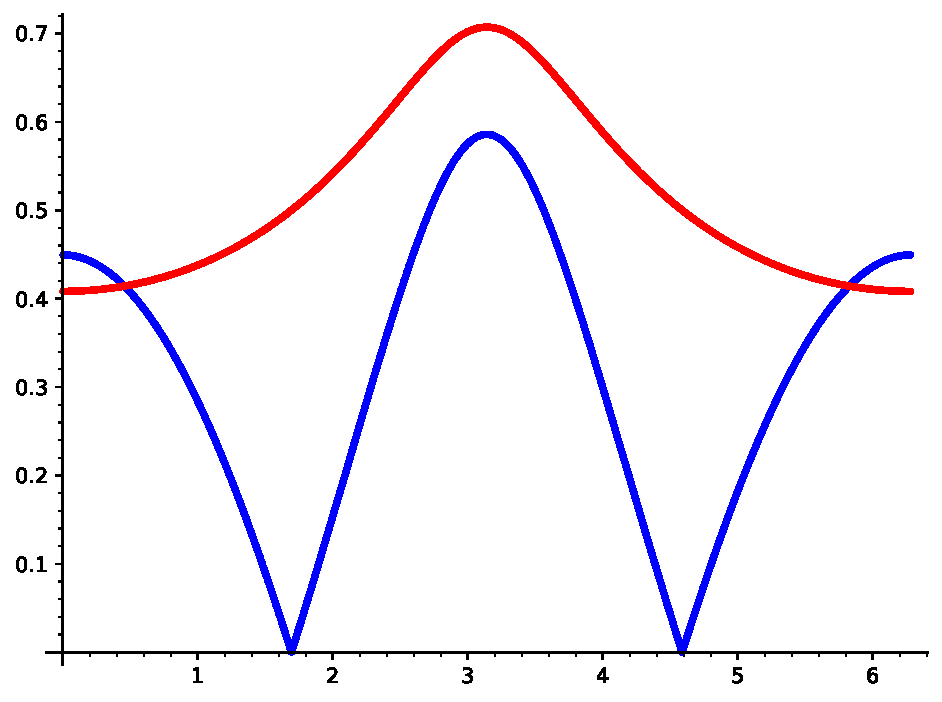
\includegraphics[width=5cm]{fig_sqrt.pdf}}
  \caption{Graph of $|\Re \sqrt{1+z}-1|/|z|$ (in blue) and
    $|\Im \sqrt{1+z}|/|\Im z|$ (in red), for $z = e^{i t}/2$,
    $0 \le t \le 2\pi$.} \label{fig_sqrt}
\end{figure}

\begin{proof}
  See Fig.~\ref{fig_sqrt}, which considers the case where $|u|=1/2$,
  which is the worst case.
  The larger values for both the real part
  and the imaginary part are obtained when $t$ approaches $\pi$,
  i.e., when $u$ approaches $-1/2$.
\begin{comment}
lre=[]
lim=[]
k=1001
r=1/2
for j in [0..2*k]:
   z=n(r*exp(i*j*pi/k))
   if z!=0 and imag(z)!=0:
      re=abs(real(sqrt(1+z)-1))
      im=abs(imag(sqrt(1+z)))
      lre.append((j*pi/k,re/abs(z)))
      lim.append((j*pi/k,im/abs(imag(z))))
p=list_plot(lre,color='blue')+list_plot(lim,color='red')
p.save("fig_sqrt.pdf")
\end{comment}
\end{proof}

Now $\sqrt{z'} = \sqrt{z} \cdot \sqrt{1+\epsilon/z}$.
Define $u := \epsilon/z$:
$|\epsilon| \le \sqrt{2^{-2p} (x^2 + y^2)} = 2^{-p} |z|$,
thus $|u| \le 2^{-p}$.
Applying Lemma~\ref{lem:sqrtaux}
yields $|\Re \sqrt{1+u}-1| \le 0.6 |u|$ and
$|\Im\sqrt{1+u}| \le 0.8 |\Im u|$.
Now if $z = r e^{i\alpha}$ in polar coordinates,
$\sqrt{z} = \sqrt{r} e^{i\alpha/2}$, and it follows that
$|\Im\sqrt{z}/\Re\sqrt{z}| = |\tan(\alpha/2)| \le |\tan(\alpha)|
\le |\Im z/\Re z| < 2^{-k}$.
If $\sqrt{z} = a+ib$ and $\sqrt{1+u} = (1+c)+id$, we obtain
$|b/a| < 2^{-k}$, $|c| \le 0.6 \cdot 2^{-p}$, $|d| \le 0.8 |\Im(u)|$.

Let $\epsilon = \epsilon_x + i \epsilon_y$, then
\[ \epsilon/z = (\epsilon_x + i \epsilon_y)/(x + iy) =
  (\epsilon_x + i \epsilon_y)(x-iy)/|z|^2
  = \frac{\epsilon_x x + \epsilon_y y}{|z|^2}
  + i \frac{-\epsilon_x y + \epsilon_y x}{|z|^2}. \]
Therefore $\Im(u) = (-\epsilon_x y + \epsilon_y x)/|z|^2$,
and $|\Im(u)| \le 2^{-p+1} |x| |y|/|z|^2$.
Since $|y/x| < 2^{-k}$, $|\Im(u)| \le 2^{-p-k+1}$,
thus $|d| \le 0.8 \cdot 2^{-p-k+1}$.

When multiplying $\sqrt{z}$ by $\sqrt{1+u} = (1+c)+id$, we get:
\[ \sqrt{z + \epsilon} = \sqrt{z} + \sqrt{z}  (c + i d). \]
The induced error is thus:
\[ \sqrt{z}  (c + i d) = (a + ib) (c + i d). \]
Its real part is bounded by:
\[ |ac| + |bd| \le (0.6 \cdot 2^{-p} + 0.8 \cdot 2^{-p-2k+1}) |a|
  \le 2^{-p} \cdot |a|, \]
and its imaginary part is bounded by:
\[ |ad| + |bc| \le (0.8 \cdot 2^{-p-k+1} + 0.6 \cdot 2^{-p-k}) |a|
  < 2.2 \cdot 2^{-p-k} \cdot |a|. \]
We have proven the following lemma.
\begin{lemma} \label{lem:sqrt}
  Assume $z = x + iy$ with $|y/x| < 2^{-k}$, and $k \ge 1$.
  Let $z' = z + \epsilon$ with $|\Re\epsilon| < 2^{-p} |x|$
  and $|\Im\epsilon| < 2^{-p} |y|$, for $p \ge 1$.
  Then $\sqrt{z'} = \sqrt{z} + \tau$ with:
  \[ |\Re\tau| \le 2^{-p} |\Re\sqrt{z}|, \quad
     |\Im\tau| \le 2^{-p-k+1} |\Re\sqrt{z}|. \]
\end{lemma}

\section {Complex analysis}

\begin {theorem}[Taylor expansion and remainder term]
\label {th:taylor}
Let $f : U \to \C$ be a holomorphic function on the open subset
$U \subseteq \C$. Denote by $B = B (c, r) = \{ z \in \C : |z - c| < r \}$
the open disk with centre~$c$ and radius~$r$, by
$\overline B = \overline B (c, r) = \{ z \in \C : |z - c| \leq r \}$
its closure, and by
$\partial B = \partial B (c, r) = \{ z \in \C : |z - c| = r \}$
its boundary. Assume that $\overline B \subseteq U$, and let $z \in B$.
Let $M_r = \max\limits_{w \in \partial B} |f (w)|$,
let $\beta$ be any real number such that $|z - c| / r \leq \beta < 1$,
and let $N \geq 1$ be an integer. Then
\[
f (z) = f (c) + \sum_{n = 1}^N \frac {f^{(n)} (c)}{n!} (z - c)^n + R_N
\text { with }
|R_N| \leq M_r \, \frac {\beta^{N + 1}}{1 - \beta}.
\]
\end {theorem}
\begin {proof}
The Taylor series for $f$ is given by \cite [Theorem~16-8]{Apostol57} as
\[
f (z) = f (c) + \sum_{n = 1}^\infty \frac {f^{(n)} (c)}{n!} (z - c)^n
\]
under the sole assumption that $B \subseteq U$.
Cauchy's integral formula gives the remainder term by
\cite [Theorem~16-7]{Apostol57} as
\[
R_N = \sum_{n = N+1}^\infty \frac {f^{(n)} (c)}{n!} (z - c)^n
= \sum_{n = N+1}^\infty \frac {(z - c)^n}{2 \pi i}
\int\limits_{w \in \partial B} \frac {f (w)}{(w - c)^{n+1}} \, \diff w
\]
under the assumption that $\overline B \subseteq U$.
So
\[
|R_N| \leq \sum_{n = N+1}^\infty \frac {|z - c|^n}{2 \pi}
\int\limits_{w \in \partial B} \frac {M_r}{r^{n+1}} \, \diff w
= M_r \sum_{n = N+1}^\infty \left( \frac {|z - c|}{r} \right)^n
\leq M_r \sum_{n = N+1}^\infty \beta^n,
\]
and evaluating the geometric series yields the bound of the theorem.
\end {proof}

\begin {remark}
The result probably still holds when $f$ is holomorphic only
on~$B \subseteq U$ instead of on $\overline B$, assuming that it is at
least continuous on $\partial B$ (in particular, it is not allowed to have
a singularity on the boundary); a proof idea would be to apply the theorem
for $r' < r$ and to take the limit $r' \to r$.
We do not need such a result, and instead can apply this approach to upper
bounds obtained in cases we are interested in.
\end {remark}

We also need a special case in which the remainder term can be bounded
trivially.

\begin {theorem}
\label {th:taylorpositive}
In the situation of Theorem~\ref {th:taylor}, assume that $c = 0$ and
$z \in B$. Write
$c_n = f^{(n)} (0) / n!$ and
$f_N (z) = \sum_{n=0}^N c_n z^n$.
Assume that the $c_n$ for $n > N$ are real and either all non-negative,
or all non-positive. Then
\[
f (z) = f_N (z) + R_N
\]
with
\[
|R_N| \leq \frac {|f (r) - f_N (r)|}{r^{N+1}} \, |z|^{N+1}.
\]
\end {theorem}

\begin {proof}
By definition, we have $R_N = g_N (z)$ with
$g_N (z) = \sum_{n = N+1}^\infty c_n z^n$, so that
$|R_N| \leq \sum_{n=N+1}^\infty |c_n| \, |z|^n$,
or
$|R_N| \leq C_N |z|^{N+1}$
with
\[
C_N = \frac {\sum_{n=N+1}^\infty |c_n| \, |z|^n}{|z|^{N+1}}
    = \sum_{n=N+1}^\infty |c_n| \, |z|^{n - (N+1)}.
\]
Since all the occurring $c_n$ are either non-negative or non-positive,
the left-hand expression shows that
\[
C_N = \frac {|g_N (|z|)|}{|z|^{N+1}}
    = \frac {|f (|z|) - f_N (|z|)|}{|z|^{N+1}}.
\]
The right-hand expression shows that it is a real power-series with
non-negative coefficients, so it is increasing as a real function and
for $z \in B$ bounded above by its value in~$r$, which implies the
desired formula.
\end {proof}




\section {Algorithms}
\label {sec:algorithms}

This section describes in detail the algorithms used in \mpc, together with
the error analysis that allows to prove that the results are correct in the
{\mpc} semantics: The input numbers are assumed to be exact, and the output
corresponds to the exact result rounded in the desired direction.


\subsection {\texttt {mpc\_sqrt}}

The following algorithm is due to Friedland \cite{Friedland67,Smith98}.
Let $z = x + i y$.

Let $w = \sqrt { \frac {|x| + \sqrt {x^2 + y^2}}{2}}$ and
$t = \frac {y}{2w}$. Then $(w + it)^2 = |x| + iy$, and with the branch cut on the negative real axis we obtain
\[
\sqrt z = \left\{
\begin {array}{cl}
w + i t & \text {if } x > 0 \\
t + i w & \text {if } x < 0, y > 0 \\
-t - i w & \text {if } x < 0, y < 0
\end {array}
\right.
\]

Jeannerod and Muller prove in \cite{jeannerod:ensl-01780265} that the relative
error of this algorithm --- with rounding to nearest ---
is at most $\frac{5}{2} u$ for the real part, denoted
$w$ here, and
$\frac{7}{2} u$ for the imaginary part, denoted $t$ here,
where $u = 2^{-p}$ and $p$ is the
working precision.
However, this is not sufficient to be able to compute the ternary value,
for which a directed rounding is preferred.
We thus reuse the error analysis of that paper using directed roundings.

With the notations of \cite{jeannerod:ensl-01780265}, and denoting RD for
rounding down (for $t > 0$), equation (5) becomes:
\[ t (1 - \frac{2u}{1+2u}) \leq {\rm RD}(t) \]
% \[ {\rm RU}(t) \leq t (1 + 2u), \]
since --- assuming without loss of generality $1 \leq t < 2$ ---
the worst case is when $t$ is just below ${\rm nextafter}(1) = 1+2u$.
% and worst case for RU is attained for $t$ just above $1$.
The same bounds apply both for additions and multiplications, as in equation (5)
from \cite{jeannerod:ensl-01780265}, but also for the square root and division,
as in equations (6) and (7).
The lower bound $L'$ from equation (9) then becomes:
\[ L' = (1 - \delta_d)^{5/2} \] % U' = (1 + \delta_u)^{5/2}
with $\delta_d = 2u/(1+2u)$. % and $\delta_u = 2u$.
% var('u')
% delta_d = 2*u/(1+2*u); delta_u = 2*u
% taylor((1-delta_d)^(5/2), u, 0, 3)
% -105/2*u^3 + 35/2*u^2 - 5*u + 1
% taylor((1+delta_u)^(5/2), u, 0, 3)
% 5/2*u^3 + 15/2*u^2 + 5*u + 1
It follows from a Taylor expansion of $L'$:
\[ 1 - 5u \leq L'. \]

Assume $x > 0$, let $w$ be the exact real part of
$\sqrt{z}$, and $\hat{w}$ be the approximate value computed by
Friedland's algorithm.
We thus have $0 \leq w - \hat(w) \leq 5 u w$.
We claim that this bound can be converted to
$0 \leq w - \hat(w) \leq 10 \ulp(\hat(w))$.
Assume $w$ is in the binade $[2^k,2^{k+1})$, then $\hat{w}$ is either in that
binade or in $[2^{k-1},2^k)$.
Since $\ulp(w) = 2^{k+1} \cdot u$, we thus have $\ulp(\hat{w}) \geq 2^k \cdot u$ in
all cases, which yields $w - \hat(w) \leq 5 (w/2^k) \ulp(\hat{w}) \leq 10 \ulp(\hat{w})$.

Thus the total error on $w$ is at most \ulp{10}.
For the computation of $t$, assuming $y > 0$, we round upwards the division $y/(2w)$,
which yields a relative error of at most $2u$, and thus:
\[ \hat{t}/t \leq \frac{1 + \delta_u}{(1 - \delta_d)^{5/2}} = 1 + 7u + \frac{35}{2} u^2 + O(u^3), \]
with $\delta_u = 2u$,
which implies $\hat{t}/t \leq 1 + 8u$ for $p \geq 5$.
% taylor((1+delta_u)/(1-delta_d)^(5/2), u, 0, 3)
% 35/2*u^3 + 35/2*u^2 + 7*u + 1
As above, this implies $\hat{t} - t \leq 16 \ulp(\hat{t})$.

\subsection {\texttt {mpc\_log}}

Let $z = x + i y$. Then $\log (z) = \frac {1}{2} \log (x^2 + y^2) + i \atantwo (y, x)$. The imaginary part is computed by a call to the corresponding {\mpfr} function.

Let $w = \log (x^2 + y^2)$, rounded down. The error of the complex norm is \ulp{1}. The generic error of the real logarithm is then given by \ulp{$2^{2 - e_w} + 1$}, where $e_w$ is the exponent of $w$. For $e_w \geq 2$, this is bounded by \ulp{2} or 2~digits; otherwise, it is bounded by \ulp{$2^{3 - e_w}$} or $3 - e_w$ digits.

\begin{lemma} \label{lem:logaux}
  Let $u$ be a complex number with $|u| \le 1/2$, then we have:
  \[ |\Re \log(1+u)| \le 2 \log 2 \cdot |u|,
    \quad |\Im \log(1+u)| \le 2 \cdot |\Im u|. \]
\end{lemma}
Note the bound for the real part is in terms of $|u|$, while that for the imaginary
part is in terms of $|\Im u|$.
\begin{figure}[htp]
  \centerline{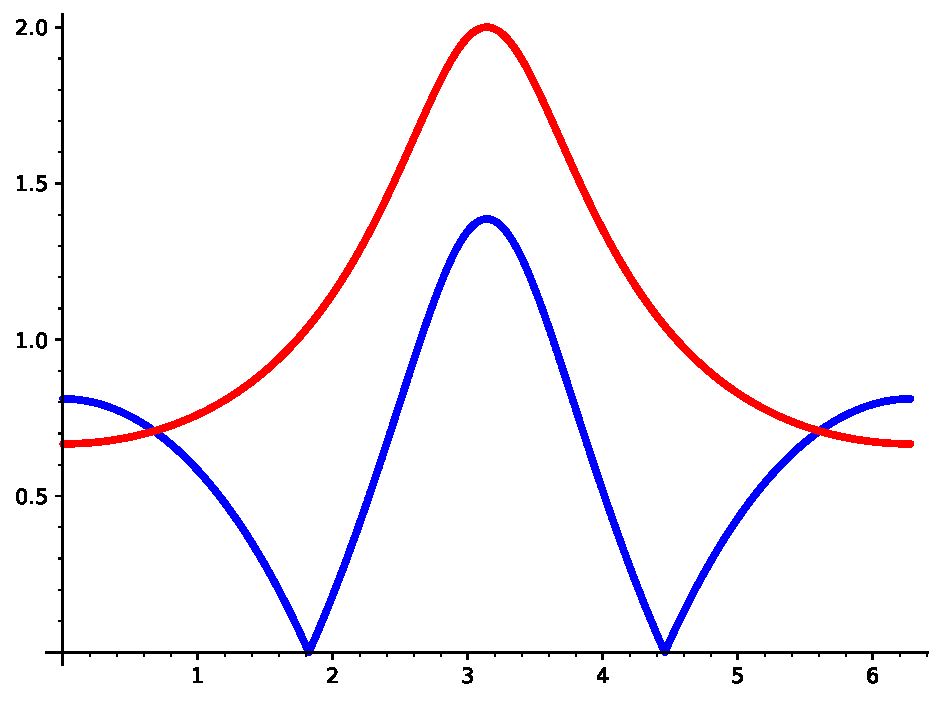
\includegraphics[width=5cm]{fig_log.pdf}}
  \caption{Graph of $|\Re \log(1+z)|/|z|$ (in blue) and
    $|\Im \log(1+z)|/|\Im z|$ (in red), for $z = e^{i t}/2$,
    $0 \le t \le 2\pi$.} \label{fig_log}
\end{figure}

\begin{proof}
  See Fig.~\ref{fig_log}, which considers the case where $|u|=1/2$,
  which is the worst case.
  The larger values for both the real part
  and the imaginary part are obtained when $t$ approaches $\pi$,
  i.e., when $u$ approaches $-1/2$.
\begin{comment}
lre=[]
lim=[]
k=1001
r=1/2
for j in [0..2*k]:
   z=n(r*exp(i*j*pi/k))
   if z!=0 and imag(z)!=0:
      re=abs(real(log(1+z)))
      im=abs(imag(log(1+z)))
      lre.append((j*pi/k,re/abs(z)))
      lim.append((j*pi/k,im/abs(imag(z))))
p=list_plot(lre,color='blue')+list_plot(lim,color='red')
p.save("fig_log.pdf")
\end{comment}
\end{proof}

\begin{lemma} \label{lem:log}
  Assume $z = x + iy$ with $|y/x| < 2^{-k}$, $k \ge 1$ and $x \ge 2$.
  Let $z' = z + \epsilon$ with $|\Re\epsilon| < 2^{-p} |x|$
  and $|\Im\epsilon| < 2^{-p} |y|$, for $p \ge 1$.
  Then $\log z' = \log z + \tau$ with:
  \[ |\Re\tau| \le 2^{-p+1} |\Re\log z|, \quad
     |\Im\tau| \le 2^{-p-k+3} |\Re\log z|. \]
\end{lemma}
\begin{proof}
  We follow the proof of Lemma~\ref{lem:sqrt}.
  We have $\log z' = \log(z + \epsilon) = \log z \cdot \log(1+\epsilon/z)$.
  Let $u = \epsilon/z$. As in the proof of Lemma~\ref{lem:sqrt},
  we have $|u| \le 2^{-p}$.
  Applying Lemma~\ref{lem:logaux} yields
  $|\Re \log(1+u)| \le 2 \log 2 \cdot |u|$ and
  $|\Im \log(1+u)| \le 2 \cdot |\Im u|$.
  Since $|u| \le 2^{-p}$ and
  as in the proof of Lemma~\ref{lem:sqrt},
  $|\Im u| \le 2^{-p-k+1}$, it follows
  $|\Re \log(1+u)| \le 2 \log 2 \cdot 2^{-p}$ and
  $|\Im \log(1+u)| \le 2^{-p-k+2}$.
  Now it is easy to check that if $x \ge 2$, then
  $|\Re\log z| \ge \log 2$, thus
  $|\Re \log(1+u)| \le 2^{-p+1} |\Re\log z|$ and
  $|\Im \log(1+u)| \le 2^{-p-k+3} |\Re\log z|$.
\end{proof}

\subsection {\texttt {mpc\_tan}}

Let $z = x + i y$ with $x \neq 0$ and $y \neq 0$.

We compute $\tan z$ as follows:
\begin{align*}
u &\leftarrow \A(\sin z) &\error(\Re(u)) &\leq 1 \Ulp(\Re(u))
&\error(\Im(u)) &\leq 1 \Ulp(\Im(u))
\\
v &\leftarrow \A(\cos z) &\error(\Re(v)) &\leq 1 \Ulp(\Re(v))
&\error(\Im(v)) &\leq 1 \Ulp(\Im(v))
\\
t &\leftarrow \A(u/v) &\error(\Re(t)) &\leq k_R \Ulp(\Re(t))
&\error(\Im(t)) &\leq k_I \Ulp(\Im(t))
\end{align*}
where $w_2 \leftarrow \A(w_1)$ means that the real and imaginary parts of
$w_2$ are respectively the real and imaginary part of $w_1$ rounded away from
zero to the working precision.

We know that $\Re(\frac{a+i b}{c+i d})=\frac{a c +b d}{c^2 + d^2}$ and
$\Im(\frac{a+i b}{c+i d})=\frac{a d -b c}{c^2 + d^2}$, so in the special case
of $\tan z=\frac{\sin x\cosh y+i\cos x\sinh y}{\cos x\cosh y-i\sin x\sinh y}$,
we have $abcd < 0$ which means that there might be a cancellation in the
computation of the real part while it does never happen in the one of the
imaginary part.  Then, using the generic error of the division (see
\ref{sssec:propdiv}), we have
\begin{align*}
\error(\Re(t)) &\leq [1+2^{3+e_1}+2^{3+e_2}+2^6] \Ulp(\Re(t)),
\\
\error(\Im(t)) &\leq [1+2^3+2^3+2^6] \Ulp(\Im(t)),
\end{align*}
where $e_1=\Exp(a c) -\Exp(a c+b d)$ and $e_2=\Exp(b d) -\Exp(a c+b d)$.  The
second inequality shows that $2^7$ is suitable choice for $k_I$. As $|\sinh
y|<\cosh y$ for every nonzero $y$, we have $bd<ac$, thus $e_2\leq e_1$. We
know that $\Exp(\frac{a c+b d}{c^2+d^2})\leq \Exp(a c+b d) -\Exp(c^2+d^2)$,
$\Exp(c^2+d^2)\geq2 \min(\Exp(c), \Exp(d))$, and $\Exp(ac) \leq \Exp(a) +
\Exp(c)$, this gives an upper bound for $e_1$:
\[
e_1 \leq e = \Exp(\Re(u)) +\Exp(\Re(v)) -\Exp(\Re(t))
-2 \min(\Exp(\Re(v)), \Exp(\Im(v))).
\]
and a suitable value for $k_R$:
\begin{equation*}
k_R=\left\{
\begin{array}{l l}
  2^7 & \mbox{if $e < 2$;}
  \\
  2^8 & \mbox{if $e = 2$}
  \\
  2^{5 + e} & \mbox{else.}
\end{array}
\right.
\end{equation*}

\subsection {\texttt {mpc\_asin}}

Besides non-finite, real and purely imaginary arguments, we treat a few
special cases separately to speed up the computations.
We use \texttt {\mpc\_asin} as the basis for other inverse trigonometric and
hyperbolic functions, since \texttt {mpc\_asinh} and \texttt {mpc\_acos}
as well as \texttt {mpc\_acosh} (through \texttt {mpc\_acos}) may be reduced
to a computation of \texttt {mpc\_asin}. So improvements to this function
will be immediately beneficial to the others.

\paragraph{Tiny imaginary part with real part $1$.}
First, in case the real part of the argument is exactly $1$,
for $0 \leq y \leq 1$, we have $|\Re \asin (1 \pm iy) - \pi/2|
\leq y^{1/2}$, and $|\Im \asin (1 \pm iy) \mp y^{1/2}| \leq (1/12) y^{3/2}$.

\paragraph{Tiny imaginary part with real part $x^2 \le 1/2$.}
Assume $|y| < 2^k$ with $k \le -1$.
Then:
\[ \sqrt{1-z^2} = \sqrt{1-(x^2 - y^2 + 2ixy)}
  = \sqrt{1-x^2} \sqrt{1 + y^2/(1-x^2) - 2ixy/(1-x^2)}. \]
Since $$x^2 \le 1/2$ and $|y| < 2^k$,
the $y^2/(1-x^2)$ term is bounded by $2^{2k+1}$;
if we neglect it, the absolute error is bounded by $2^{2k+1}$:
\[ \sqrt{1-z^2} = \sqrt{1-x^2} \sqrt{1 - 2ixy/(1-x^2)} + \tau, \]
with $|tau| \le 2^{2k+1}$.
Now since the Taylor expansion of $\sqrt{1-t}$ is
$1 - t/2 - t^2/8 + O(t^3)$,
$\sqrt{1 - 2ixy/(1-x^2)} = 1 - ixy/(1-x^2) + \mu$
with $|\mu| < x^2 y^2/(1-x^2) \le 2^{2k}$.
It follows:
\[ iz + \sqrt{1-z^2} = i x - y + \sqrt{1-x^2} (1 - ixy/(1-x^2) + \mu) + \tau
  = (i x + \sqrt{1-x^2}) (1 - y/\sqrt{1-x^2}) + \tau', \]
with $|\tau'| \le |\sqrt{1-x^2} \mu + \tau|
\le 2^{2k-1} + 2^{2k+1} \le 2^{2k+2}$.
Let $v = (i x + \sqrt{1-x^2}) (1 - y/\sqrt{1-x^2})$ and $u = \tau'/v$.
Assume $|x| \ge 2^e$, then $|v| \ge 2^e (1 - 2^k) \ge 2^{e-1}$,
thus $|u| \le 2^{2k+2}/2^{e-1} = 2^{2k-e+3} \le 1/2$ as long as $2k-e \le -4$.
Then according to Lemma~\ref{lem:logaux}, 
$|\Re \log(1+u)| \le 2 \log 2 |u|$,
and $|\Im \log(1+u)| \le 2 |\Im u|$,
thus $|\log(1+u)| \le \sqrt{4 \log^2 2 + 4} |u| \le 3 \cdot 2^{2k-e+3}$.
We now have:
\[ \asin z = i \log(v + \tau')
  = i \log v + i \log(1 + u)
  = i \log (i x + \sqrt{1-x^2}) + i \log(1 - y/\sqrt{1-x^2}) + i \log(1+u)
  = \asin x + i \log(1 - y/\sqrt{1-x^2}) + i \log(1+u). \]
Now $|y/\sqrt{1-x^2}| \le 2^{k+1}$, and since the Taylor expansion of
$\log(1+t)$ is $t - t^2/2 + O(t^3)$, we have
$\log(1 - y/\sqrt{1-x^2}) = - y/\sqrt{1-x^2} + \nu$ with
$|\nu| \le y^2/(1-x^2) \le 2^{2k+1}$.
It follows the following lemma.
\begin{lemma} \label{lem:asin2}
  Let $z = x + iy$ with $2^e \le x \le \sqrt{2}/2$, $|y| < 2^k$ with $k \le -1$.
  Then
\[ \asin z = \asin x + iy/\sqrt{1-x^2} + \nu', \]
with $|\nu'| \le 2^{2k-e+5}$.
\end{lemma}
\begin{proof}
  From the above reasoning, we have $\nu' = \nu + i \log(1+u)$,
  thus $|\nu'| = |\nu + i \log(1+u)| \le 2^{2k+1} + 3 \cdot 2^{2k-e+3}$.
  Now since $2^e \le \sqrt{2}/2$, we have $e \le -1$, thus
  $2^{2k+1} + 3 \cdot 2^{2k-e+3} \le 2^{2k-e+3} + 3 \cdot 2^{2k-e+3} = 2^{2k-e+5}$.
\end{proof}  

\paragraph{Small real and imaginary parts.}
Formula 4.4.40 from \cite{AbSt73} gives for $|z| < 1$:
\begin{equation} \label{eq_asin1}
  \asin z = \sum_{k \geq 0} \frac{1 \times 3 \times \cdots \times (2k-1)}
  {2 \times 4 \times \cdots \times (2k)} \frac{z^{2k+1}}{2k+1}.
\end{equation}
When $|\Re z|,|\Im z| \leq 2^e$ with $e \leq -11$,
we can use the following algorithm, with working precision $p$:
\begin{verbatim}
   w = o(z*z)
   t = o(z)
   s = o(z)
   for k from 1 to K-1 do:
      u = o(t * w)
      v = o(u * ((2k-1) * (2k-1)))
      t = o(v / ((2*k) * (2*k+1))
      s = s + t
\end{verbatim}
We first prove by induction that at the end of the for loop with index $k$,
we have (up to rounding errors):
\[ t = \frac{1  \times 3 \times \cdots \times (2k-1)}
  {2 \times 4 \times \cdots \times (2k)} \frac{z^{2k+1}}{2k+1}. \]
This is easy and left to the reader.
Then since $|\Re z|,|\Im z| \leq 2^e$,
we have $|\Re(w)|,|\Im(w)| \leq o(2^{1+2e}) = 2^{1+2e}$.

Then we prove, still by induction, that at the end of the for loop with index
$k$, we have $|\Re(t)|,|\Im(t)| \leq 2^{2k+(2k+1)e}$.
This holds for $k=0$, i.e., at the beginning of the loop with $k=1$,
since then $t$ is the rounding of $z$,
thus $|\Re t|,|\Im t| \leq o(2^e) = 2^e$,
since $2^e$ is exactly representable.
Now assume $|\Re(t)|,|\Im(t)| \leq 2^{2k-2+(2k-1)e}$ at the beginning of the
loop with index $k$.
Since $|\Re(w)|,|\Im(w)| \leq 2^{1-2e}$, we have after the first instruction
in the loop: $|\Re(u)|, |\Im(u)| \leq 2^{2k+(2k+1)e}$. After the second
instruction, we get $|\Re(v)|, |\Im(v)| \leq (2k-1)^2 \cdot 2^{2k+(2k+1)e}$,
assuming $(2k-1)^2$ is exactly representable, which can be checked a
posteriori. Since in the third instruction we divide by $(2k)(2k+1)$
which is larger than $(2k-1)^2$, we get at the end of the loop with index $k$:
$|\Re(t)|, |\Im(t)| \leq 2^{2k+(2k+1)e}$ as claimed.

Now let $\varepsilon_k$ be the maximal absolute error on $\Re t, \Im t$ at the
end of the loop with index~$k$.
For $k=0$, i.e., at the beginning of the loop with $k=1$, we have
$\varepsilon_0 = 2^{e-p}$, since $t = o(z)$, and the error is at most
$\frac{1}{2} \Ulp(z) \leq \frac{1}{2} \Ulp(2^e) = 2^{e-p}$.
Now the absolute error on $u$ is bounded by:
\[ {\rm err}(u) \leq \frac{1}{2} \Ulp(u) + 2 \varepsilon_{k-1} |w| + 2 |t| {\rm err}(w), \]
where ${\rm err}(w)$ stands for the maximal absolute error on $w$ (i.e.,
on its real and imaginary parts), the factors $2$ come from the fact
that the real and imaginary parts of a product are a sum of two products,
and $|x|$ is a shortcut for ${\rm max}(|\Re x|, |\Im x|)$.
Since $|\Re u|, |\Im u| \leq 2^{2k+(2k+1)e}$, we have
$\frac{1}{2} \Ulp(u) \leq 2^{2k+(2k+1)e-p}$;
we also have $|w| \leq 2^{1-2e}$ and ${\rm err}(w) \leq \frac{1}{2}
\Ulp(w) \leq 2^{1-2e-p}$. This gives:
\[ {\rm err}(u) \leq 2^{2k+1+(2k+1)e-p} + 2^{2-2e} \varepsilon_{k-1}. \]
For the second instruction of the loop:
\[ {\rm err}(v) \leq \frac{1}{2} \Ulp(v) + (2k-1)^2 {\rm err}(u), \]
and for the third one:
\[ {\rm err}(t) \leq \frac{1}{2} \Ulp(t) + \frac{{\rm err}(v)}{(2k)(2k+1)}, \]
thus:
\[ \varepsilon_k \leq \frac{1}{2} \Ulp(t) +
  \frac{1}{2(2k)(2k+1)} \Ulp(v) + \frac{(2k-1)^2}{(2k)(2k+1)} {\rm err}(u). \]
For the first term of the right-hand side,
$\frac{1}{2} \Ulp(t) \leq 2^{2k+(2k+1)e-p}$;
the last one is bounded by ${\rm err}(u)$;
using $|v| \leq (2k-1)^2 \cdot 2^{2k+(2k+1)e}$, and
the rule $\Ulp(ab) < 2 |a| \Ulp(b)$,
the middle one is bounded by
\[ \frac{1}{2(2k)(2k+1)} \Ulp(v) \leq
  \frac{(2k-1)^2}{(2k)(2k+1)} \Ulp(2^{2k-(2k+1)e})
  \leq 2^{2k+1+(2k+1)e-p}. \]
This yields:
\[ \varepsilon_k \leq 2^{2k+(2k+1)e-p} + 2^{2k+1+(2k+1)e-p}
  + 2^{2k+1+(2k+1)e-p} + 2^{2+2e} \varepsilon_{k-1}
  \leq 5 \cdot 2^{2k+(2k+1)e-p} + 2^{2+2e} \varepsilon_{k-1}. \]
We distinguish two cases: $e=-1$ or $e \leq -2$.
For $e=-1$ we get:
\[ \varepsilon_k \leq 5 \cdot 2^{-1-p} + \varepsilon_{k-1}, \]
thus since $\varepsilon_0 = 2^{-1-p}$ we have
$\varepsilon_k \leq (5k+1) 2^{-1-p}$.
For $e \leq -2$, we have for $k \geq 1$:
\[ \varepsilon_k \leq 5 \cdot 2^{-2+e-p} + \frac{1}{4} \varepsilon_{k-1}, \]
and it follows easily $\varepsilon_k \leq \frac{5}{3} \cdot 2^{e-p}$.

Now the absolute error on $s$ at the end of the for loop --- not taking into
account the mathematical error when truncating the Taylor series ---
is bounded by:
\begin{eqnarray}
{\rm err}(s) &\leq& \sum_{k=0}^{K-1} (5k+1) 2^{-1-p} = \frac{(5K-3)K}{2} 2^{-1-p} \quad \mbox{for $e=-1$}, \label{eq:asin1} \\
{\rm err}(s) &\leq& \sum_{k=0}^{K-1} \frac{5}{3} \cdot 2^{-e-p} =
  \frac{5}{3} K 2^{-e-p} \quad \mbox{for $e \le -2$}. \label{eq:asin2}
\end{eqnarray}

\paragraph{Finer analysis for small real and imaginary parts.}
Assume $|\Re z| \le 2^{e_x}$, $|\Im z| \le 2^{e_y}$.
Let $w = z^2$.
Then if $e_x \le e_y$,
$|\Re w| \le 2^{2 e_x} + 2^{2e_y} \le 2^{2e_y+1}$,
and $|\Im w| \le 2 \cdot 2^{e_x + e_y} = 2^{e_x + e_y + 1}$.
We can prove by induction that for $k \ge 1$:
\[ |\Re z^{2k+1}| \le 2^{e_x + 2k e_y + 2k}, \quad
   |\Im z^{2k+1}| \le 2^{(2k+1) e_y + 2k} \quad \mbox{when $e_x \le e_y$}. \]
We have similar bounds when $e_y \le e_x$:
\[ |\Re z^{2k+1}| \le 2^{(2k+1) e_x + 2k}, \quad
   |\Im z^{2k+1}| \le 2^{2k e_x + e_y + 2k} \quad \mbox{when $e_y \le e_x$}. \]
 These bounds still hold for the Taylor coefficients of $\asin z$,
 since the coefficients of Eq.~(\ref{eq_asin1}) are less or equal to $1$.
 Moreover these bounds still hold with rounding, since powers of $2$ round
 to themselves.
 If $\max(e_x,e_y) \le -1$, then it follows:
\[ |\Re z^{2k+1}| \le 2^{e_x}, \quad
   |\Im z^{2k+1}| \le 1/2 \quad \mbox{when $e_x \le e_y \le -1$}, \]
\[ |\Re z^{2k+1}| \le 1/2, \quad
  |\Im z^{2k+1}| \le 2^{e_y} \quad \mbox{when $e_y \le e_x \le -1$}. \]
This shows that if one of the real (resp.~imaginary) part of $z$ is tiny,
it remains tiny for the odd powers $z^{2k+1}$, and thus for the values
of $t$ in the above algorithm.
Thus the error bounds from Eqs.~(\ref{eq:asin1}) and~(\ref{eq:asin2})
apply separately on each side: in particular for $e_x, e_y \le -2$,
the absolute error on $\Re s$ is
bounded by $\frac{5}{3} K \cdot 2^{e_x-p}$, and absolute error on $\Im s$ is
bounded by $\frac{5}{3} K \cdot 2^{e_y-p}$.

\paragraph{Case $|z|$ large with $\Im(z) < 0$.}
For any complex $z$, the sum $iz + \sqrt{1-z^2}$ lies in the right complex
plane, inside the unit circle for $\Im z > 0$, and outside it for $\Im z < 0$
(see Fig.~\ref{fig_asin}).
Therefore to avoid cancellation it is better to force $\Im z < 0$,
by reducing the argument using the formula $\asin (-z) = - \asin z$.
\begin{figure}[htp]
\begin{comment}
lpos=[]
lneg=[]
C=ComplexField(53)
for j in range(1000):
   z = C.random_element()
   t = i*z+sqrt(1-z^2)
   if imag(z)>0:
      lpos.append((real(t),imag(t)))
   else:
      lneg.append((real(t),imag(t)))
p=list_plot(lpos,color='blue')+list_plot(lneg,color='red')
p+=polar_plot(1,(x,-pi/2,pi/2),color='black')
p.save("fig_asin.pdf")
\end{comment}
  \centerline{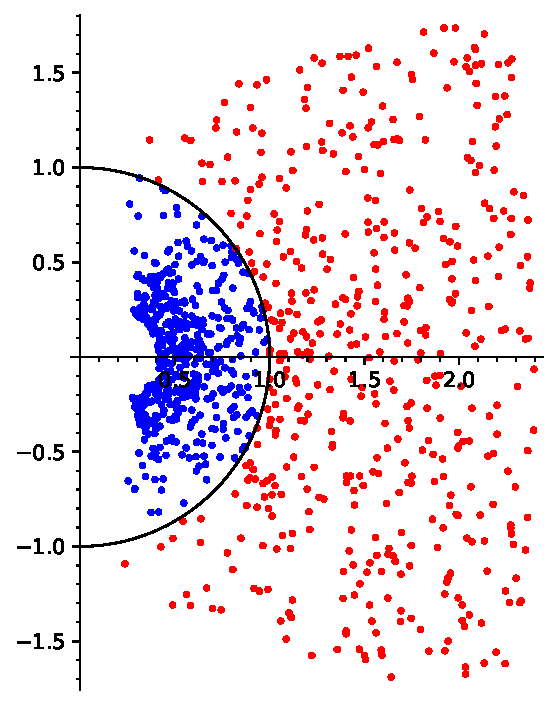
\includegraphics[width=5cm]{fig_asin.pdf}}
  \caption{Graph of $iz + \sqrt{1-z^2}$ for 1000 random values of $z$,
    in blue for $\Im{z} > 0$, and in red for $\Im{z} \le 0$, with the
    unit circle in black.} \label{fig_asin}
\end{figure}  
In the case $|z|$ large and $\Im(z) < 0$, when using the formula
\[ \asin(z) = -i \log (iz + \sqrt{1-z^2}), \]
the sum $iz + \sqrt{1-z^2}$ is close to $2iz$.
Indeed, for large $|z|$ we have $\sqrt{1-z^2} \approx iz$ when
$\Re(iz) > 0$, i.e., $\Im(z) < 0$.
We first prove the following lemma.
\begin{lemma} \label{lemma17}
  Assume $t$ complex with $|t| \leq 1/4$, then
  \[ \sqrt{1-t} = 1 + \varepsilon, \]
  with $|\varepsilon| < |t|$.
\end{lemma}
\begin{figure}[htp]
\begin{comment}
l=[]
r=1/4
k=1001
for j in range(2*k):
   t = n(r*exp(i*j*pi/k))
   u = sqrt(1-t)-1
   l.append((j*pi/k,abs(u)/abs(t)))
p=list_plot(l,color='blue')
p.save("fig_lemma17.pdf")
\end{comment}
  \centerline{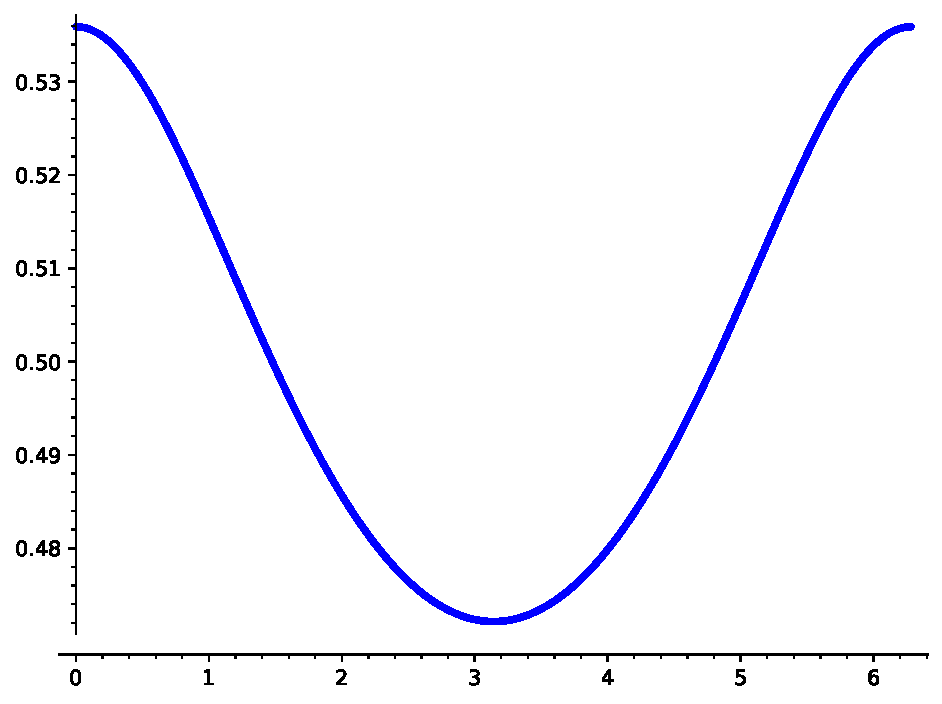
\includegraphics[width=5cm]{fig_lemma17.pdf}}
  \caption{Graph of $|\sqrt{1-t}-1|/|t|$ for
    $t = e^{iu}/4$, $0 \le u \le 2\pi$.} \label{fig_lemma17}
\end{figure}  

\begin{proof}
  We see on Figure~\ref{fig_lemma17}, which considers the worst case
  $|t| = 1/4$, that the maximum of $|\sqrt{1-t}-1|/|t|$
  is obtained for $u$ near $0$ or $2\pi$,
  i.e., $t = 1/4$, and this maximum is less than $0.54 < 1$.
\end{proof}

Applying this lemma to $t = 1/z^2$, as long as $|z| \ge 2$, we get:
\[ iz + \sqrt{1-z^2} = iz + iz \sqrt{1-1/z^2}
  = 2iz + iz \epsilon \quad
  \mbox{with $|\varepsilon| < 1/|z^2|$.} \]
Thus if we approximate $iz + \sqrt{1-z^2}$ by $2iz$,
the relative error is bounded by $1/|2z^2|$.

Let $e_z = {\rm max}(\Exp(\Re(z)),\Exp(\Im(z)))$.
Then $|z| \ge 2^{e_z-1}$ thus $|2z^2| > 2^{2e_z-1}$.
The relative error is bounded by $1/|2z^2| < 2^{-2e_z+1}$,
thus by Prop.~\ref{prop:relerror} it is less than $2^{-2e_z+p+1}$ ulps,
where $p$ is the working precision, and we assume $p \ge 4$.
We further assume $2e_z \ge p+1$, so that this relative error is bounded
by 1 ulp.

We then form $t = 2iz = x + iy$, this is exact.

We then compute $u = {\tt mpc\_log}(t)$.
We have
\[ \log t = \frac{1}{2} \log(x^2+y^2) + i \, {\rm atan2}(y,x). \]
We analyze separately the induced error on the real and imaginary parts
of $u \approx \log t$.

For the real part, the relative error when approximating
$iz + \sqrt{1-z^2}$ by $2iz$ is less than $2^{-p}$.
This gives a relative error less than $(1 + \cdot 2^{-p})^2 - 1 < 2.1 \cdot 2^{-p}$
on $x^2$ and $y^2$, and similarly for $x^2+y^2$.
Now we deduce the relative error on $\log(x^2+y^2)$.
Let $U = x^2+y^2$ and $V$ the corresponding exact value;
we have shown that $U = V (1 + \varepsilon)$ with
$|\varepsilon| < 2.1 \cdot 2^{-p}$.
It follows $\log U = \log V + \log(1 + \varepsilon)$
with $|\log(1 + \varepsilon)| < 2.3 \cdot 2^{-p}$.
Since $|x|, |y| < 2^{e_t}$, we have $x^2+y^2 < 2^{2e_t+1} \le 2^{-2e_z+1}
\le 2^{-p+1}$ since $2e_z \ge p$.
Thus $|\log(x^2+y^2)| \ge (p-1) \log 2$,
and the relative error on $\log(x^2+y^2)$ is bounded by
$2.3 \cdot 2^{-p}/((p-1) \log 2) < 1.2 \cdot 2^{-p}$.
The same holds for $1/2 \log(x^2+y^2)$, thus the relative error on $\Re(u)$
is bounded by $1.2 \cdot 2^{-p}$, thus by $3$ ulps, taking into account
the rounding error in \verb|mpc_log|.

For the imaginary part, since $\Im(z) < 0$, $z$ is either in the 3rd or 4th
quadrant, and we can check that $2iz$ lies in the 1st or 4th
quadrant, thus ${\rm atan2}(y,x)$ lies in $(-\pi/2,\pi/2)$, and in both
cases ${\rm atan2}(y,x) = {\rm atan}(y/x)$.
Similarly to the real part, the error from the approximation by $2iz$
induces a relative error less than $2^{-p}$ on $x$ and $y$,
thus a relative error less than $(1 + 2^{-p})^2-1 < 2.1 \cdot 2^{-p}$
on $y/x$.
Since the derivative of $\rm atan$ is less than $1$, this corresponds
to a relative error less than $2.1 \cdot 2^{-p}$ on $\Im(u)$,
thus less than $3$ ulps like for the real part,
taking into account the rounding error of \verb|mpc_log|.


\subsection {\texttt {mpc\_pow}}

The main issue for the power function is to be able to recognize when the
real or imaginary part of $x^y$ might be exact, since in that case
Ziv's strategy will loop infinitely.
If both parts of $x^y$ are known to be inexact, then we use
$x^y = \exp(y \log x)$ and Ziv's strategy.
After computing an integer $q$ such that $|y \log x| \leq 2^q$, we first
approximate $y \log x$ with precision $p + q$, and then
$\exp(y \log x)$ with precision $p \geq 4$, all with rounding
to nearest.
Let $\tilde{s} = \round_{p+q}(\log x)$,
we have $\tilde{s} = (\log x) (1 + \theta_1)$
with $\theta_1$ a complex number of norm $\leq 2^{-p-q}$.
Let $\tilde{t} = \round_{p+q}(y \tilde{s})$, then
$\tilde{t} = y \tilde{s} (1 + \theta_2) = (y \log x) (1 + \theta_3)^2$,
where $\theta_2, \theta_3$ are complex numbers of norm $\leq 2^{-p-q}$,
thus $|\tilde{t} - y \log x| \leq 2.5 \cdot 2^{-p}$ for $q \geq -3$.
Now $\tilde{u} = \round_p(\exp(\tilde{t})) =
x^y \exp(2.5 \cdot 2^{-p}) (1 + \theta_4) = x^y (1 + 4 \theta_5)$,
with $\theta_4, \theta_5$ complex numbers of norm $\leq 2^{-p}$.

In the remainder of this section, we determine the cases where at
least one part of $x^y$ is exact, and for that, we assume $x$ to be
different from the trivial cases $0$ and $1$.

\begin {definition}
A {\em dyadic real} is a real number $x$ that is exactly representable
as a floating point number, that is, $x = m \cdot 2^e$ for some $m$, $e \in \Z$.
A {\em dyadic complex} or {\em dyadic}, for short, is a complex number
$x = x_1 + i x_2$ with both $x_1$ and $x_2$ dyadic reals.
\end {definition}

Recall that $\Z [i]$, the ring of Gaussian integers or integers of $\Q (i)$,
is a principal ideal domain with units
$\Z [i]^\ast = \{ \pm 1, \pm i \} = \langle i \rangle$,
in which $2$ is ramified: $(2) = (2 i) = (1 + i)^2$. Let $p_0 = 1 + i$, and
$p_k$ for $k \geq 1$ the remaining primes of $\Z [i]$. Then any element
$x$ of $\Q (i)$ has a unique decomposition as
$x = i^u \prod_{k \geq 0} p_k^{\alpha_k}$ with $u \in \{ 0, 1, 2, 3\}$,
$\alpha_k \in \Z$ and almost all $\alpha_k$ equal to zero.

\begin {prop}
\label {prop:dyadic}
The dyadics are precisely the $p_0$-units of $\Q (i)$, that is,
the numbers $x = i^u \prod_{k \geq 0} p_k^{\alpha_k}$
such that $\alpha_k \geq 0$ for $k \geq 1$.
\end {prop}

\begin {proof}
This follows immediately from the fact that $p_k^{-1}$ for $k \geq 1$ is not
dyadic, while $p_0^{-1} = \frac {1 - i}{2}$ is.
\end {proof}

Gelfond-Schneider's theorem states that if $x$ and $y$ are algebraic and
$y$ is not rational, then $x^y$ is transcendental.
Since all dyadic complex numbers are algebraic, this implies that $x^y$ is
not dyadic whenever $y$ has a non-zero imaginary part.
Unfortunately, this does not rule out the possibility that
either the real or the imaginary part of $x^y$ might still be dyadic,
while the other part is transcendental.
For instance, $i^y$ is real for $y$ purely imaginary, so that
also $x^y$ is real for $x \in \Z [i]^\ast$ and $y$ purely imaginary.

\begin {conj}
\label{conj}
If $\Im y \neq 0$ and $x$ is not a unit of $\Z [i]$, then
the real and the imaginary part of $x^y$ are transcendental.
Or, more weakly, then neither the real nor the imaginary
part of $x^y$ are dyadic reals.
\end {conj}

We then need to examine more closely the case of $y$ a dyadic real,
and we first concentrate on positive $y$.

\begin{lemma}
\label{lemma1}
Let $x$ be a dyadic complex and $m 2^e$ a positive dyadic real
with $m \in \Z_{>0}$, $m$ odd and $e \in \Z$.
Then $x^{m 2^e}$ is a dyadic complex if and only if $x^{2^e}$ is.
\end{lemma}

\begin{proof}
Notice that by Proposition~\ref {prop:dyadic} the set of dyadics forms
a ring, whence any positive integral power of a dyadic is again dyadic.
Thus if $x^{2^e}$ is dyadic, then so is $x^{m 2^e}$.

Conversely, assume that $x^{m 2^e}$ is dyadic. If $e \geq 0$,
then $x^{2^e}$ is dyadic independently of the assumption,
and it remains to consider the case $e < 0$.

Write $x = i^u \prod_{k \geq 0} p_k^{\alpha_k}$
and $z = x^{m 2^e} = i^v \prod_k p_k^{\beta_k}$, so that $x^m = z^{2^{|e|}}$.
The uniqueness of the prime decomposition implies that
$m \alpha_k = 2^{|e|} \beta_k$, and since $m$ is odd, $2^{|e|}$ must
divide $\alpha_k$. Then
$x^{2^e} = i^w \prod_k p_k^{\gamma_k}$ with $w \equiv m^{-1} v \pmod 4$ and
$\gamma_k = \frac {\alpha_k}{2^{|e|}}$.
Now $\alpha_k \geq 0$ for $k \geq 1$ implies $\gamma_k \geq 0$ for $k \geq 1$,
and $x^{2^e}$ is dyadic by Proposition~\ref {prop:dyadic}.
\end{proof}

It remains to decide when $x^{2^e}$ is dyadic for $x$ dyadic. If $e \geq 0$,
this is trivially the case. For $e < 0$, the question boils down to whether
it is possible to take $e$ successive square roots of $x$; as soon as the
process fails, it is clear that $x^{2^e}$ cannot be dyadic.

\begin{lemma}
\label {lm:sqrtrat}
Let $x \in \Q (i)$, and write $x = (a + b i)^2$ with $a$, $b \in \R$.
Then either both of $a$ and $b$ are rational, or none of them is.
\end{lemma}

\begin{proof}
Assume that one of $a$ and $b$ is rational. Then $\Im x = 2 a b \in \Q$
implies that also the other one is rational.
\end{proof}

\begin{lemma}
Let $x$ be dyadic, and write $x = (a + b i)^2$ with $a$, $b \in \R$.
Then either both of $a$ and $b$ are dyadic reals, or none of them is.
\end{lemma}

\begin{proof}
Assume that one of $a$ and $b$ is a dyadic real, that is, a rational with
a power of~$2$ as denominator. Then $a$, $b \in \Q$ by Lemma~\ref {lm:sqrtrat}.
Now, $\Re x = a^2 - b^2$ implies that also the square of the \textit {a priori}
not dyadic coefficient $a$ or $b$, and thus the coefficient itself,
has as denominator a power of~$2$.
\end{proof}


\begin {theorem}
Let $x = m 2^e$ and $y = n 2^f$ be dyadic complex numbers with $m$ and $n$ odd,
and let $z = x^y$. Call the pair $(x, y)$ {\em exceptional} if at least
one of $\Re z$ or $\Im z$ is a dyadic real. Exceptional pairs occur
only in the following cases:
\begin {enumerate}
\item
$y = 0$; then $z = 1$
\item
$x \geq 0$ and $y \neq 0$ are real; then $\Im z = 0$, and the question
whether $\Re z = x^y$ is dyadic involves only real numbers and
can thus be delegated to \mpfr.
\item
$x < 0$ and $y \neq 0$ are real.
\begin {enumerate}
\item
$y \in \Z$; then $\Im z = 0$, and $\Re z = x^y$ is dyadic if and only if
$y > 0$, or $y < 0$ and $-m = 1$.
\item
$y \in \frac {1}{2} \Z \backslash \Z$, that is, $f = -1$;
then $\Re z = 0$, and $\Im z = (-x)^y$ is dyadic if and only if
$e$ is even, $-m$ is a square, and, in case $y < 0$, $-m = 1$.
\item
$y \in \frac {1}{4} \Z \backslash \frac {1}{2} \Z$, that is, $f = -2$;
then $z = \frac {1 + i}{\sqrt 2} (-x)^y$ has both real and imaginary
dyadic parts if and only if
$e \equiv 2 \pmod 4$, $-m$ is a fourth power, and, in case $y < 0$, $-m = 1$.
\end {enumerate}
\item
$y$ not real;
see Conjecture~\ref {conj}
\item
$y > 0$ real, $x$ not real;
see above
\item
$y < 0$ real, $x$ not real;
still to do
\end {enumerate}
\end {theorem}

\begin {proof}
\begin {enumerate}
\item
Clear by definition.
\item
Clear.
\item
The first two subcases $f \geq -1$ follow from the observation that
$x^y = (-1)^y (-x)^y$, where $(-1)^y \in \langle i \rangle$.
For $y > 0$, the number $(-x)^y$ is dyadic if and only if $(-x)^{2^f}$ is,
which leads to the result; for $y < 0$, one furthemore needs that
$(-m)^{-1}$ is dyadic, which for $m$ odd is only possible if $-m = 1$.
The third subcase $f = -2$ is similar, but one needs that $(-x)^y$ is dyadic
up to a factor of $\sqrt 2$.

We proceed to show that for $f \leq -3$, there is no exceptional pair.
Suppose that $(x, y)$ is an exceptional pair; by switching to
$\left( x^{|n|}, \frac {y}{|n|} \right)$, we may assume
without loss of generality that $|n| = 1$. Then $x^y$ is obtained by
taking $|f|$ successive square roots of either $x$ or $\frac {1}{x}$, both
of which are elements of $\Q (i)$. Lemma~\ref {lm:sqrtrat} implies
that both $\Re (x^y)$ and $\Im (x^y)$ are rational.

Write $x^y = \alpha \zeta = \alpha \zeta_r + i \alpha \zeta_i$, where
$\alpha = (-x)^y \in \R$ and $\zeta = \zeta_r + i \zeta_i$ is a primitive root
of unity of order~$2^{|f| + 1}$.
Then $\alpha \zeta_r$, $\alpha \zeta_i \in \Q$ implies $\zeta \in \Q (i, \alpha)$.
Moreover,
$\alpha^2 = \alpha^2 (\zeta_r^2 + \zeta_i^2) =
(\alpha \zeta_r)^2 + (\alpha \zeta_i)^2 \in \Q (i)$, so that $\Q (i, \alpha)$
is an extension of degree at most~$4$ of $\Q$ containing $\Q (\zeta)$
and thus a primitive $16$-th root of unity, which is impossible.
\item
\item
\item
\end {enumerate}
\end {proof}

\paragraph{Sign of zeroes.}
When the output value has a zero real or imaginary part, its sign should be
decided, which is not always possible if we want it to be consistent with the
formula $x^y = \exp(y\log x)$ (in the following, we exclude $0^y$).

Let $x_1$, $x_2$, $y_1$, and $y_2$ real numbers so that $x = x_1 + x_2 i$ and
$y = y_1 + y_2 i$.
Let $\phi \in [-\pi, +\pi]$ the argument of $x = |x| e^{i\phi}$, with the
convention that when $x_1 < 0$ the argument of $x$ is $+\pi$ if $x_2 = +0$ and
$-\pi$ if $x_2 = -0$.
Then
\[
x^y=\exp\left(A(x,y)\right) \left(\cos B(x,y)+\sin B(x,y) i\right)
\] where
\begin {align*}
  A(x,y) & =  y_1\log|x|-y_2\phi,\\
  B(x,y) & =  y_2\log|x|+y_1\phi.
\end {align*}
As $|x^y| = \exp\left(A(x,y)\right)$ is positive, the value of $B(x,y)$
determines the sign of each part of $x^y$.
Note that $A(\overline{x},y) = A(x,\overline{y})$ and $B(\overline{x},
y)=-B(x,\overline{y})$, so $\overline{x}^y = \overline{x^{\overline{y}}}$ and
we can restrict the study below to $x$ with nonnegative imaginary value
(i.e., $x_2 \geq 0$ and $\pi \geq \phi \geq 0$).

To determine the sign of the zero part of $x^y$ when it is pure real or pure
imaginary, special study is needed around points $(x, y)$ where $B(x, y)$ is a
multiple of $\pi/2$.
Let
\begin {equation}
  \label {eqn:Bk}
  B_k(x, y) = y_2 \log|x| +y_1\phi -k\frac{\pi}{2}
\end {equation}
where $k$ is an integer and let $S_k$ the set of points $(x, y)$ where $B_k(x,
y) = 0$.

For any integer $k$, we assume that the surface $S_k$ is orientable and not
reduced to a single point, then each neighborhood of a point $(x_0, y_0)$ of
$S_k$ intersects the region where $B(x, y) > k\pi/2$ and the region where $B(x,
y) < k\pi/2$.
Thus for an even $k$, we can make $(x, y)$ tend continuously to $(x_0, y_0)$
so that $\Re(x^y) > 0$ or we can make it tend to $(x_0, y_0)$ so that
$\Re(x^y) < 0$ (the same applies with $k$ odd and $\Im(x^y)$).
In such cases, the sign of the zero part of $x_0^{y_0}$ is not determined.

However, when $S_k$ intersects an axis, for example when $\Re(x_0) = 0$, we
have to distinguish two cases: $\Re(x_0) = +0$ and $\Re(x_0) = -0$.
Then, if $Q_{x_0}$ (resp. $Q_{y_0}$) denotes the quadrant where $x_0$
(resp. $y_0$) lies, it is possible that the sign of $B_k(x,y)$ remains
constant for $(x,y)$ in the intersection $I$ of a neighborhood of $(x_0, y_0)$
with $Q_{x_0}\times Q_{y_0}$, determining the sign of the zero part of $x^y$.
Let $dB_k(x,y)$ be the derivative of $B_k(x, y)$, we have
\begin {equation}
  \label {eqn:BkDerivative}
  dB_k(x, y)\cdot(\delta_1, \delta_2, \epsilon_1, \epsilon_2) =
  \frac{x_1y_2-x_2y_1}{x_1^2+x_2^2}\delta_1 +
  \frac{x_1y_1+x_2y_2}{x_1^2+x_2^2}\delta_2 +
  \phi\epsilon_1 +
  \log|x| \epsilon_2
\end {equation}
If $dB_k(x_0, y_0)\cdot(\delta_1, \delta_2, \epsilon_1, \epsilon_2)$ is not
zero and if its sign remains constant for all real numbers $\delta_1$,
$\delta_2$, $\epsilon_1$, and $\epsilon_2$ so that $x = x_0 + \delta_1 +
\delta_2i$, $y = y_0 +\epsilon_1 + \epsilon_2i$, and $(x,y)$ is in the given
neighborhood $I$ of $(x_0, y_0)$ defined above, then the sign of $dB_k(x_0,
y_0)\cdot(\delta_1, \delta_2, \epsilon_1, \epsilon_2)$ determines the sign of
the zero part of $x^y$.

In following discussion, we write
$B_k(x_1, x_2, y_1, y_2) := B_k(x_1+x_2i, y_1+y_2i)$,
as a function of four real arguments.
Let $\sigma_1 = -1,+1$ (resp. $\sigma_2$, $\rho_1$, $\rho_2$) denote the sign
of $x_1$ (resp. $x_2$, $y_1$, $y_2$).
\begin {enumerate}
\item Case $B_k(\sigma_1 0, x_2, y_1, y_2)=0$ for $x_2 > 0$.
  Here $\phi = +\frac{\pi}{2}$.
  \begin {enumerate}
  \item if $y_2=\rho_2 0$, then replacing $\phi$ and $y_2$ by their value in
    (\ref{eqn:Bk}), we have $y_1= k$ and (\ref{eqn:BkDerivative}) gives
    \[
    dB_k(\sigma_1 0, x_2, k, \rho_2 0)\cdot(\delta_1, \delta_2, \epsilon_1,
    \epsilon_2) = - \frac{k}{x_2} \delta_1 + 0 \delta_2 + \frac{\pi}{2}
    \epsilon_1 + \log(x_2) \epsilon_2
    \]
    where $\sigma_1 \delta_1 > 0$, and $\rho_2 \epsilon_2 > 0$ so that
    $\delta_1 + (x_2 + \delta_2)i$ (resp. $k+\epsilon_1 + \epsilon_2 i$) is in
    the same quadrant $Q_{x_0}$ (resp.  $Q_{y_0}$) as $x_0=\sigma_1 0 +x_2 i$
    (resp. $y_0=k +\rho_2 0i$).

    When $k \neq 0$, because, in the last expression,
    $\epsilon_1$ would take positive as well as negative values,
    so the sign of $\frac{\pi}{2} \epsilon_1$, and therefore the sign of
    $dB_k(x, y)\cdot (\delta_1, \delta_2, \epsilon_1, \epsilon_2)$ is not
    constant.

    If $k=0$, then $y_1=\rho_1 0$ with $\rho_1 \epsilon_1 > 0$.
    In this case,
    \begin {align*}
      dB_0(\pm 0, x_2, +0, +0)\cdot(\delta_1, \delta_2, \epsilon_1,
      \epsilon_2) &> 0 \;\text{if}\; x_2 \geq 1 \\
      dB_0(\pm 0, x_2, +0, -0)\cdot(\delta_1, \delta_2, \epsilon_1,
      \epsilon_2) &> 0 \;\text{if}\; 1 \geq x_2 > 0 \\
      dB_0(\pm 0, x_2, -0, -0)\cdot(\delta_1, \delta_2, \epsilon_1,
      \epsilon_2) &< 0 \;\text{if}\;  x_2 \geq 1 \\
      dB_0(\pm 0, x_2, -0, +0)\cdot(\delta_1, \delta_2, \epsilon_1,
      \epsilon_2) &< 0 \;\text{if}\; 1 \geq x_2 > 0
    \end {align*}
    and the sign of $dB_k(\sigma_1 0, x_2, \rho_1 0, \rho_2 0)\cdot(\delta_1,
    \delta_2, \epsilon_1, \epsilon_2)$ is not constant in all other
    combinations of $k$, $\sigma_1$, $x_2>0$, $\rho_1$, and $\rho_2$.

  \item if $y_2\neq 0$, then from (\ref{eqn:Bk})
    \[
    x_2 = \exp\left(\frac{k-y_1}{2y_2}\pi\right).
    \]
    But the number in the right hand side of the last equation is
    known to be transcendental unless $k-y_1=0$.
    As $x_2$ is dyadic, we have $y_1= k$ and $x_2=+1$.
    Using (\ref{eqn:BkDerivative}), we write
    \[
    dB_k(\sigma_1 0, +1, k, y_2)\cdot(\delta_1, \delta_2, \epsilon_1,
    \epsilon_2) = - k \delta_1 + y_2 \delta_2 + \frac{\pi}{2} \epsilon_1 + 0
    \epsilon_2
    \]
    where $\sigma_1 \delta_1 > 0$.

    Here, $\delta_2$ can take negative and positive values preventing the sign
    of $dB_k(\sigma_1 0, +1, k, y_2)\cdot (\delta_1, \delta_2, \epsilon_1,
    \epsilon_2)$ from being constant.
  \end {enumerate}

\item Case $B_k(x_1, +0, y_1, y_2)=0$ with $x_1 \neq 0$.
      (Remember we assumed $x_2 \geq 0$.]
  \begin {enumerate}
  \item if $x_1 >0$, then $\phi = +0$.
    From (\ref{eqn:Bk}), we have
    \[
    y_2 \log x_1 = k \frac{\pi}{2}.
    \]
    \begin {enumerate}
    \item if $y_2 = \rho_2 0$, the last equation implies $k = 0$, and from
      (\ref{eqn:BkDerivative}) we have
      \[
      dB_0(x_1, +0, y_1, \rho_2 0)\cdot(\delta_1, \delta_2, \epsilon_1,
      \epsilon_2) = 0 \delta_1 + \frac{y_1}{x_1} \delta_2 + 0 \epsilon_1 +
      \log(x_1) \epsilon_2
      \]
      with $\delta_2 > 0$ and $\rho_2 \epsilon_2 > 0$.

      The sign of the last expression in constant only in the following
      cases,
      \begin {align*}
        dB_0(x_1, +0, y_1, +0)\cdot(\delta_1, \delta_2, \epsilon_1,
        \epsilon_2) &> 0 \;\text{if}\; y_1 \geq 0 \;\text{and}\; x_1 > 1\\
        dB_0(+1, +0, y_1, \pm 0)\cdot(\delta_1, \delta_2, \epsilon_1,
        \epsilon_2) &> 0 \;\text{if}\; y_1 > 0\\
        dB_0(x_1, +0, y_1, -0)\cdot(\delta_1, \delta_2, \epsilon_1,
        \epsilon_2) &> 0 \;\text{if}\; y_1 \geq 0 \;\text{and}\; 1 > x_1 > 0 \\
        dB_0(x_1, +0, y_1, -0)\cdot(\delta_1, \delta_2, \epsilon_1,
        \epsilon_2) &< 0 \;\text{if}\; y_1 \leq 0 \;\text{and}\; x_1 > 1\\
        dB_0(+1, +0, y_1, \pm 0)\cdot(\delta_1, \delta_2, \epsilon_1,
        \epsilon_2) &< 0 \;\text{if}\; y_1 < 0\\
        dB_0(x_1, +0, y_1, +0)\cdot(\delta_1, \delta_2, \epsilon_1,
        \epsilon_2) &< 0 \;\text{if}\; y_1 \leq 0 \;\text{and}\; 1 > x_1 > 0.
      \end {align*}
      Notice that we cannot conclude when $dB_0(x,y)$ is identically zero,
      so the cases $x=+1+0i$, $y=y_1 \pm0i$ cannot be determined by this
      means.

    \item If $y_2 \neq 0$, then $x_1 = \exp\left(\frac{k}{2y_2}\pi\right)$
      is a dyadic number only if $k=0$ and then $x_1=1$.
      We have, using (\ref{eqn:BkDerivative}),
      \[
      dB_0(+1, +0, y_1, y_2)\cdot(\delta_1, \delta_2, \epsilon_1,
      \epsilon_2) = y_2 \delta_1 + y_1 \delta_2 + 0 \epsilon_1 + 0
      \epsilon_2
      \]
      with $\delta_2 > 0$.

      Here $y_2 \delta_1$ can take negative as well as positive values
      preventing the sign of $dB_0(+1, +0, y_1, y_2)\cdot(\delta_1,
      \delta_2, \epsilon_1, \epsilon_2)$ from being constant.
    \end {enumerate}

  \item if $x_1 < 0$, then $\phi = \pi$.
    Using (\ref{eqn:BkDerivative}), we have
    \[
    dB_k(x_1, +0, y_1, y_2)\cdot(\delta_1, \delta_2, \epsilon_1, \epsilon_2)
    = \frac{y_2}{x_1} \delta_1 + \frac{y_1}{x_1} \delta_2 + \pi \epsilon_1 +
    \log(-x_1) \epsilon_2
    \]
    with $\delta_2 > 0$.

    If $y_1 \neq 0$, then $\epsilon_1$ can take negative as well as positive
    values, preventing $dB_k$ from having a constant sign.
    Assume thus $y_1 = 0$.
    As $x_1 \neq 0$, $\delta_1$ can also take negative and positive values,
    and $-y_2 \delta_1$ does not have a constant sign unless $y_2 = 0$.
    But from \ref {eqn:Bk}, we know that $B_k(x, 0)=0$ implies $k = 0$
    since $x_1 = - \exp(\frac{k \pi}{2 y_2})$ is dyadic.

    When $y = 0$, the derivative of $B_k$ is
    \[
    dB_0(x_1, +0, \rho_1 0, \rho_2 0)\cdot(\delta_1, \delta_2, \epsilon_1,
    \epsilon_2) = 0 \delta_1 + 0 \delta_2 + \pi \epsilon_1 + \log(-x_1)
    \epsilon_2
    \]
    with $\delta_2 >0$, $\rho_1 \epsilon_1 >0$ and $\rho_2 \epsilon_2 >0$.

    Then,
    \begin {align*}
      dB_0(x_1, +0, +0, +0)\cdot(\delta_1, \delta_2, \epsilon_1,
      \epsilon_2) &> 0 \;\text{if}\; x_1 \leq -1 \\
      dB_0(x_1, +0, +0, -0)\cdot(\delta_1, \delta_2, \epsilon_1,
      \epsilon_2) &> 0 \;\text{if}\; -1 \leq x_1 < 0 \\
      dB_0(x_1, +0, -0, -0)\cdot(\delta_1, \delta_2, \epsilon_1,
      \epsilon_2) &< 0 \;\text{if}\; x_1 \leq -1\\
      dB_0(x_1, +0, -0, +0)\cdot(\delta_1, \delta_2, \epsilon_1,
      \epsilon_2) &< 0 \;\text{if}\; -1 \leq x_1 < 0
    \end {align*}
    and the sign of $dB_k(x_1, +0, \rho_1 0, \rho_2 0)\cdot(\delta_1,
    \delta_2, \epsilon_1, \epsilon_2)$ is not constant in all other
    combinations of $k$, $x_1<0$, $\rho_1$, and $\rho_2$.
  \end {enumerate}

\item Case $B_k(x_1, x_2, \rho_1 0, y_2)=0$ for $x_2 \geq 0$.
  Here, we have
  \[
  y_2\log|x|-k\frac{\pi}{2} = 0.
  \]
  \begin{enumerate}
  \item If $y_2=0$, then from the last equation $k=0$.
    Using (\ref{eqn:BkDerivative})
    \[
    dB_0(x_1,x_2,\rho_10,\rho_20)\cdot(\delta_1, \delta_2, \epsilon_1, \epsilon_2) =
    0\delta_1 + 0\delta_2 + \phi \epsilon_1 +\log|x| \epsilon_2
    \]
    where $\rho_1 \epsilon_1 > 0$ and $\rho_2 \epsilon_2 > 0$.

    The case $\phi = 0$, that is $x_1 > 0$ and $x_2 = 0$, has already been
    processed above in Case (b)(i).
    Let $\phi > 0$, then $x_2$ is not zero or $x_1 < 0$.
    Using the expression of the derivative given above, we have
    \begin{align*}
      dB_0(x_1, x_2, +0, +0)\cdot(\delta_1, \delta_2, \epsilon_1, \epsilon_2)
      &> 0 \;\text{if}\; |x| \geq 1 \;\text{and}\; \pi \geq \phi > 0\\
      dB_0(x_1, x_2, -0, -0)\cdot(\delta_1, \delta_2, \epsilon_1, \epsilon_2)
      &< 0 \;\text{if}\; |x| \geq 1 \;\text{and}\; \pi \geq \phi > 0\\
      dB_0(x_1, x_2, +0, -0)\cdot(\delta_1, \delta_2, \epsilon_1, \epsilon_2)
      &> 0 \;\text{if}\; 1 \geq |x| > 0 \;\text{and}\; \pi \geq \phi > 0\\
      dB_0(x_1, x_2, -0, +0)\cdot(\delta_1, \delta_2, \epsilon_1, \epsilon_2)
      &< 0 \;\text{if}\; 1 \geq |x| > 0 \;\text{and}\; \pi \geq \phi > 0
    \end{align*}
  \item If $y_2 \neq 0$, from (\ref{eqn:Bk}), we have
    \[
    |x|=\exp\left(\frac{k\pi}{2y_2}\right).
    \]
    The right hand side of the equation is known to be transcendental
    unless $k=0$.
    As the left hand side is dyadic, we have $k=0$, and then $|x|=1$.
    Here, (\ref{eqn:BkDerivative}) gives
    \[
    dB_0(x_1,x_2,\rho_10,y_2)\cdot(\delta_1, \delta_2, \epsilon_1, \epsilon_2)
    = x_1y_2\delta_1 + x_2y_2\delta_2 + \phi \epsilon_1 + 0\epsilon_2
    \]
    with $\rho_1 \epsilon_1 > 0$.

    If $x_2 \neq 0$, then $x_2y_2\delta_2$ can take negative as well as
    positive values and the sign of the derivative is not constant.
    Assume thus $x_2 = 0$.
    Then, $x_1=\pm 1$ because $|x|=1$, and $x_1y_2\delta_1$ can take negative
    and positive values.

    So, the sign of the zero part of $B_k(x_1, x_2, \pm 0, y_2)$ (if any)
    cannot be determined for all integers $k$ and for all dyadic real numbers
    $x_1$, $x_2$, and $y_2 \neq 0$.
  \end{enumerate}

\item If $B_k(x_1, x_2, y_1, \rho_2 0)=0$ for $x_2 \geq 0$.
  The case $y_1=0$ has already been precessed above in Case (c).
  Let $y_1 \neq 0$, then from (\ref{eqn:Bk}) we have
  \[
  \phi = \frac{k}{2y_1}\pi
  \]
  which implies that the argument $\phi$ of $x$ can be written as $r \pi$ for
  some rational number $r$ and, in the same time, $\cos^2 \phi =
  x_1^2/|x|^2$ and $\sin^2 \phi = x_2^2/|x|^2$ are rational.

  The five only possibilities (with $x_2 \geq 0$) are:\footnote{This is wrong:
 consider $\phi = \pi/3$, with $\cos \phi = 1/2$ and $\sin \phi = \sqrt{3}/2$.}
  \begin{enumerate}
  \item $\phi = 0$, but then $x_2=0$.
    This case has been processed above.
  \item $\phi = \frac{\pi}{4}$, then $x_1 = x_2 > 0$.
    From (\ref{eqn:Bk}), we have $y_1 = 2k \neq 0$, and from
    (\ref{eqn:BkDerivative})
    \[
    dB_k(x_1, x_1, 2k, \rho_2 0)\cdot(\delta_1, \delta_2, \epsilon_1,
    \epsilon_2) = -\frac{k}{x_1}\delta_1 + \frac{k}{x_1}\delta_2 +
    \frac{\pi}{4}\epsilon_1 + \log(\sqrt{2}x_1)\epsilon_2
    \]
    with $\rho_2\epsilon_2>0$.

    As $x_1 \neq 0$ and $k \neq 0$, the term $\frac{k}{x_1}\delta_1$, and
    $dB_k(x_1, x_1, 2k, \rho_2 0)\cdot(\delta_1, \delta_2, \epsilon_1,
    \epsilon_2)$ as well, has no constant sign.
  \item $\phi = \frac{\pi}{2}$, then $x_1 = 0$.
    This case has been processed above in Case (a).
  \item $\phi = \frac{3\pi}{4}$, then $x_1 = -x_2$, $x_1 < 0$ and
    (\ref{eqn:Bk}) gives $k \neq 0$ and $y_1 = \frac{2k}{3}$.
    As $y_1$ is a dyadic number, the only compatible values for $k$ are
    multiple of 3.
    Let $n$ be a nonzero integer so that $k = 3n$ and $y_1 = 2n$.
    From (\ref{eqn:BkDerivative}), we have
    \[
    dB_{3n}(-x_2, x_2, 2n, \rho_2 0)\cdot(\delta_1, \delta_2, \epsilon_1,
    \epsilon_2) = -\frac{n}{x_2}\delta_1 - \frac{n}{x_2}\delta_2 +
    \frac{3\pi}{4}\epsilon_1 + \log(\sqrt{2}x_2)\epsilon_2
    \]
    with $\rho_2\epsilon_2 >0$.

    As $n \neq 0$, $\epsilon_1$ can take negative and positive values and
    the term $\frac{3\pi}{4}\epsilon_1$ has not a constant sign.
  \item $\phi = \pi$, then $x_1<0$ and $x_2 = 0$.
    This case has been processed above in Case (b).
  \end{enumerate}
\end {enumerate}

To sum up using the inequalities above and deriving those with negative $x_2$
from them and from the relation $\overline{x}^y =
\overline{x^{\overline{y}}}$, we can give the almost complete list of complex
powers of numbers (for dyadic complex) that have a determined signed zero
part, the only exception being $x=+1 \pm 0i$ raised to zero power which cannot
be treated as we have done here.

\begin{tabular}{r@{ $=$ }lr@{ $=$ }ll}
  $x^{+0 +0i}$ & $1 +0i$,&
  $x^{-0 -0i}$ & $1 -0i$ &
  if $|x|>1$ and $x_2>0$\\
  $x^{-0 +0i}$ & $1 +0i$,&
  $x^{+0 -0i}$ & $1 -0i$ &
  if $|x|>1$ and $x_2<0$\\

  $(x_1 \pm 0i)^{\pm0 +0i}$ & $1 +0i$,&
  $(x_1 \pm 0i)^{\pm0 -0i}$ & $1 -0i$ &
  if $x_1>1$\\

  $(x_1 +0i)^{+0 +0i}$ & $1 +0i$, &
  $(x_1 +0i)^{-0 -0i}$ & $1 -0i$ &
  if $|x_1|>1$\\
  $(x_1 -0i)^{-0 +0i}$ & $1 +0i$, &
  $(x_1 -0i)^{+0 -0i}$ & $1 -0i$ &
  if $|x_1|>1$\\

  $(x_1 +0i)^{y_1 +0i}$ & $x_1^{y_1} +0i$, &
  $(x_1 -0i)^{y_1 -0i}$ & $x_1^{y_1} -0i$ &
  if $x_1>1$ and $y_1>0$\\
  $(x_1 -0i)^{y_1 +0i}$ & $x_1^{y_1} +0i$, &
  $(x_1 +0i)^{y_1 -0i}$ & $x_1^{y_1} -0i$ &
  if $x_1>1$ and $y_1<0$\\

  $(+1 +0i)^{y_1 \pm0i}$ & $1 +0i$, &
  $(+1 -0i)^{y_1 \pm0i}$ & $1 -0i$ &
  if $y_1>0$\\
  $(+1 -0i)^{y_1 \pm0i}$ & $1 +0i$, &
  $(+1 +0i)^{y_1 \pm0i}$ & $1 -0i$ &
  if $y_1<0$\\

  $x^{+0 -0i}$ & $1 +0i$, &
  $x^{-0 +0i}$ & $1 -0i$ &
  if $1>|x|>0$ and $x_2>0$\\
  $x^{-0 -0i}$ & $1 +0i$, &
  $x^{+0 +0i}$ & $1 -0i$ &
  if $1>|x|>0$ and $x_2<0$\\

  $(x_1 \pm0i)^{\pm0 -0i}$ & $1 +0i$, &
  $(x_1 \pm0i)^{\pm0 +0i}$ & $1 -0i$ &
  if $1 > x_1 > 0$ \\

  $(x_1 +0i)^{+0 -0i}$ & $1 +0i$, &
  $(x_1 -0i)^{+0 +0i}$ & $1 -0i$ &
  if $1 > |x_1| > 0$ \\
  $(x_1 -0i)^{-0 -0i}$ & $1 +0i$, &
  $(x_1 +0i)^{-0 +0i}$ & $1 -0i$ &
  if $1 > |x_1| > 0$ \\

  $(x_1 +0i)^{y_1 -0i}$ & $x_1^{y_1} +0i$, &
  $(x_1 -0i)^{y_1 +0i}$ & $x_1^{y_1} -0i$ &
  if $1 > x_1 > 0$ and $y_1 > 0$ \\
  $(x_1 -0i)^{y_1 -0i}$ & $x_1^{y_1} +0i$, &
  $(x_1 +0i)^{y_1 +0i}$ & $x_1^{y_1} -0i$ &
  if $1 > x_1 > 0$ and $y_1 < 0$ \\

  $(\pm 0 +x_2i)^{+0 +0i}$ & $1 +0i$, &
  $(\pm 0 +x_2i)^{-0 -0i}$ & $1 -0i$ &
  if $x_2 \geq 1$ \\
  $(\pm 0 +x_2i)^{+0 -0i}$ & $1 +0i$, &
  $(\pm 0 +x_2i)^{-0 +0i}$ & $1 -0i$ &
  if $1 \geq x_2 > 0$ \\
  $(\pm 0 +x_2i)^{-0 -0i}$ & $1 +0i$, &
  $(\pm 0 +x_2i)^{+0 +0i}$ & $1 -0i$ &
  if $ 0 > x_2 \geq -1$ \\
  $(\pm 0 +x_2i)^{-0 +0i}$ & $1 +0i$, &
  $(\pm 0 +x_2i)^{+0 -0i}$ & $1 -0i$ &
  if $-1 \geq x_2$ \\

  $(-1 +0i)^{+0 \pm0i}$ & $1+0i$, &
  $(-1 +0i)^{-0 \pm0i}$ & $1-0i$ \\
  $(-1 -0i)^{-0 \pm0i}$ & $1+0i$, &
  $(-1 -0i)^{+0 \pm0i}$ & $1-0i$ \\
\end{tabular}

So when $x^y$ is a pure real number, the following pattern is compatible with
the determined cases:

\begin{tabular}{rl}
  $x^y = x_1^{y_1} + \rho_2 0i$ & if $|x| > 1$\\
  $x^y = 1 + \sigma_2 \rho_1 0i$ & if $|x| = 1$\\
  $x^y = x_1^{y_1} - \rho_2 0i$ & if $|x| < 1$\\
  $x^y = x_1^{y_1} + \sigma_2 \rho_1 0i$ & if $y_1 \neq 0$
\end{tabular}

where $\sigma_2$ (resp $\rho_1$, $\rho_2$) is the sign of $x_2$ (resp. $y_1$,
$y_2$) and with the convention $0^0=+1$.

FIXME: This misses the cases $(x_1 \pm x_1 i)^{y_1 + 0 i}$ for $y_1 \geq 2$
even and $x_1 \neq 0$; the case (d)(ii) above applies when $x_2 > 0$, but
misses $x_2 < 0$. In any case, the sign of the imaginary part
(for $y_1$ divisible by~$4$)
or the real part
(for $y_1$ divisible by~$2$, but not by~$4$)
cannot be determined.


\subsection {\texttt {mpc\_pow\_ui}}
\label {ssec:mpcpowui}

In the case of a positive integer exponent $n$, it may be faster to use
binary exponentiation to compute $x^n$. More generally, let
$n_1, \ldots, n_k$ be an addition chain for $n$, that is, $n_1 = 1$,
$n_k = n$, and for any index $2 \leq r \leq k$, there are indices
$1 \leq s, t \leq r-1$ such that $n_r = n_s + n_t$. Define the corresponding
powers of $x$ as $\corr x_r = x^{n_r}$, so that $\corr x_1 = x$,
$\corr x_k = x^n$ and $\corr x_r = \corr x_s \corr x_t$.
The special case of left-to-right binary exponentiation
satisfies that $n_{r+1} = 2 n_r$ (which occurs $\lfloor \log_2 n \rfloor$
times) or $n_{r+1} = n_r + 1$ (which occurs once less than the number of
$1$ in the binary expansion of $n$, or equivalently, once less than the
Hamming weight of $n$); so $k \leq 2 \lfloor \log_2 n \rfloor + 1$.

Instead of the correct sequence $\corr x_r$, we compute during the algorithm
approximations $\appro x_1 = x = \corr x_1$ and
$\appro x_r = \round (\appro x_s \appro x_t)$
at some precision~$p$.
Let $\theta_r$ be such that $\corr x_r = \appro x_r (1 + \theta_r)$, so that
the relative error of $\appro x_r$ is given by $\epsilon_r = |\theta_r|$.
Write $z_r = \appro x_s \appro x_t$.
Then $\appro x_r = \round (z_r)$ and
$\corr x_r = z_r (1 + \theta_s)(1 + \theta_t)$.

Assuming rounding to nearest, the absolute real error attributable to
rounding $\Re z_r$ to $\Re \appro x_r$ is bounded by
$\frac {1}{2} \cdot 2^{\Exp (\Re z_r) - p}
\leq \frac {1}{2} \cdot 2^{\Exp (\Re \appro x_r) - p}$
by Proposition~\ref {prop:expround}, and the corresponding
relative real error is bounded by $2^{-p}$ according to
Proposition~\ref {prop:relerror}. The same holds for the imaginary part,
and Proposition~\ref {prop:comrelerror} implies that the complex
relative error is also bounded by $2^{-p}$. Otherwise said,
$z_r = \appro x_r (1 + \eta_r)$ with
some complex number $\eta_r$ such that $|\eta_r| \leq 2^{-p}$.
Putting the equations together, we obtain
$1 + \theta_r = (1 + \theta_s)(1 + \theta_t)(1 + \eta_r)$.
We can thus rewrite $1 + \theta_r$ as a product of factors of the
form $1 + \eta$ with $|\eta| \leq 2^{-p}$. Denoting by $u_r$ the
number of such factors, we thus have $u_r = u_s + u_t + 1$, from which
we deduce by induction, using $u_1 = 0 = n_1 - 1$,
that $u_r = n_r - 1$.

So the relative error of $\appro x_k$, compared to $x^n$, is given by
$|\theta_k| \leq (1 + 2^{-p})^{n-1} - 1$.
Using Propositions~\ref {prop:comrelerror}
and~\ref {prop:relerror}, this translates into an absolute error of
\[
\left( 1 + 2^{\Exp (\Im \appro x_k) - \Exp (\Re \appro x_k) + 1} \right)
\left( (1 + 2^{-p})^{n-1} - 1 \right)
2^p \Ulp (\Re \appro x_k)
\]
on the real part and of
\[
\left( 1 + 2^{\Exp (\Re \appro x_k) - \Exp (\Im \appro x_k) + 1} \right)
\left( (1 + 2^{-p})^{n-1} - 1 \right)
2^p \Ulp (\Im \appro x_k)
\]
on the imaginary part of the result.

If we further assume that $(n-1) 2^{-p} \leq 1$, then
$(1 + 2^{-p})^{n-1} - 1 \leq 2 (n - 1) 2^{-p}$,
because $(1+\varepsilon)^m-1 = \exp(m \log(1+\varepsilon)) - 1
\leq \exp(\varepsilon m) - 1 \leq 2 \varepsilon m$ as long as
$\varepsilon m \leq 1$. This gives the simplified bounds
\begin{equation} \label{eq:powui_re}
\left( 2 + 2^{\Exp (\Im \appro x_k) - \Exp (\Re \appro x_k) + 2} \right)
(n-1) \Ulp (\Re \appro x_k)
\end{equation}
on the real part and of
\begin{equation} \label{eq:powui_im}
\left( 2 + 2^{\Exp (\Re \appro x_k) - \Exp (\Im \appro x_k) + 2} \right)
(n-1) \Ulp (\Im \appro x_k)
\end{equation}
on the imaginary part.


\subsection {\texttt {mpc\_pow\_si}}

For the computation of $x^{-n}$ with $n > 0$, the analysis of
\S\ref {ssec:mpcpowui} essentially carries through. We keep the same
notation. Using bounds on the absolute errors of $\Re z_r$ and $\Im z_r$,
we have shown above, using Propositions~\ref {prop:relerror}
and~\ref {prop:comrelerror}, that $z_r = \appro {x_r} (1 + \eta_r)$ with
$|\eta_r| \leq 2^{-p}$ and concluded that
$x^n = \corr {x_k} = \appro {x_k} (1 + \theta_k)$, where
$1 + \theta_k$ is the product of $n-1$ factors of the form
$1 + \eta$  with $|\eta| \leq 2^{-p}$.
By exchanging the roles of $z_r$ and $\appro {x_r}$ and applying
Propositions~\ref {prop:relerror} and~\ref {prop:comrelerror}
analogously, we obtain that $z_r = \frac {\appro {x_r}}{1 + \zeta_r}$ with
$|\zeta_r| \leq 2^{-p}$ and
$x^n = \corr {x_k} = \frac {\appro {x_k}}{1 + \xi_k}$, where
$\xi_k$ is the product of $n-1$ factors of the form
$1 + \zeta$  with $|\zeta| \leq 2^{-p}$.

Let $\corr {x_{k+1}} = \corr {x_k}^{-1} = x^{-n}$ be the desired
result, $z_{k+1} = \appro {x_k}^{-1}$
and $\appro {x_{k+1}} = \round (z_{k+1})$. As shown in \S\ref {ssec:mpcpowui},
rounding of $z_{k+1}$ to the nearest implies that
$z_{k+1} = \appro {x_{k+1}} (1 + \eta_{k+1})$ with
$|\eta_{k+1}| \leq 2^{-p}$.
Then $\corr {x_{k+1}} = \frac {1}{x_k}
= \frac {1 + \xi_k}{\appro {x_k}}
= z_{k+1} (1 + \xi_k)
= \appro {x_{k+1}} (1 + \xi_k)(1 + \eta_{k+1})$,
which contains $n$ factors of the form $1 + \eta$ with
$|\eta| \leq 2^{-p}$.

Thus, assuming that $n 2^{-p} \leq 1$, the error estimates
\eqref {eq:powui_re} and \eqref {eq:powui_im} are valid with $n$
in the place of $n - 1$.


\subsection {\texttt {mpc\_rootofunity}}

Consider co-prime integers $n > 0$ and $k \geq 0$. We wish to compute
the primitive $n$-th root of unity $e^{2 \pi i k / n}$.
First, we compute $\pi$ with rounding to nearest and an absolute error
of \ulp{0.5}. Using Proposition~\ref {prop:relerror} we obtain a relative
error of $\relerror (\appro {\pi}) \leq 2^{-p}$ at precision~$p$, which
would be enough for the following analysis. However, we can be a bit more
precise, knowing the first few binary digits of $\pi$: As soon as $p \geq 7$,
% for p=6, we get 25/8 < 201/2^6, for p=7 we get 101/32 > 201/2^6
we have $201/2^6 \leq \appro {\pi}$, so
\[
\relerror (\appro {\pi})
= \left| \frac {\appro {\pi} - \corr {\pi}}{\appro {\pi}} \right|
\leq 0.637 \cdot 2^{-p}.
\]
Let $r$ be the (exact) rational number $2k/n$.
Next we compute
$\appro {t} = \round (r \appro {\pi})$, as an approximation to
$\corr {t} = r \pi$, rounded to nearest.
Its absolute error is bounded as follows:
\begin {align*}
| \appro {t} - \corr {t} |
& \leq |r \appro {\pi} - r \corr {\pi}| + 0.5 \, \Ulp (\appro {t}) \\
& =  |r \appro {\pi} / \appro {t}| \cdot |\appro {t}|
     \cdot |(\appro {\pi} - \corr {\pi}) / \appro {\pi}|
     + 0.5 \, \Ulp (\appro {t}) \\
& \leq |r \appro {\pi} / \appro {t}| \cdot 2^{\Exp (\appro {t})}
     \cdot 0.637 \cdot 2^{-p} + 0.5 \, \Ulp (\appro {t}) \\
& \leq \left( \max (|r \appro {\pi} / \appro {t}|, 1) \cdot 0.637
              + 0.5 \right) \Ulp (\appro {t})
  \text { by Definition~\ref {def:ulp}}.
\end {align*}
The factor $|r \appro {\pi} / \appro {t}|$ is larger than~$1$ only if
rounding down has occurred for $|\appro {t}|$ by at most \ulp {0.5};
with $p \geq 7$, the worst case bound is then $64.5/64$,
and the absolute error is bounded by $1.15 \, \Ulp (\appro {t})$.

The result is now obtained as
\[
\appro {s} + \appro {c} \, i
\text { with }
\appro {s} = \round (\sin (\appro {t}))
\text { and }
\appro {c} = \round (\cos (\appro {t})),
\]
rounded to nearest.
By \eqref {eq:proprealcos}, the absolute error for the real part satisfies
\begin {align*}
|\appro {s} - \corr {s}|
& \leq \left( 1.15 \cdot 2^{\Exp (\appro {t}) - \Exp (\appro {s})}
   + 0.5 \right) \, \Ulp (\appro {s}) \\
& \leq \left( 1.15 \cdot 2^{3 - \Exp (\appro {s})} + 0.5 \right)
   \, \Ulp (\appro {s}) \text { since } \Exp (\appro {t}) \leq 3 \\
& \leq 2^{4 - \Exp (\appro {s})} \, \Ulp (\appro {s})
   \text { since } \Exp (\appro {s}) \leq 0,
\end {align*}
and the analogous bound holds for the imaginary part.

If $n$ is large and $k$ close to a multiple of $n/4$, then $c$ or $s$
can become small, and we lose about as many bits as given by the exponent
of $s$ or $c$. The exact minimum of $s$ and~$c$ depends on the residue
class of $n$ modulo~$4$. To simplify the argument, we consider the $4 n$-th
roots of unity, which contain the $n$-th ones, and which are symmetrically
distributed with respect to the real and imaginary axes. Then the smallest
absolute value of the real or imaginary part is given by
$\sin (2 \pi / (4 n))$. Using $\sin (x) > x - x^3 / 6$ for $x > 0$
we obtain $\Exp (\appro {s}) \geq -63$ for $n < 2^{64}$; otherwise said,
the number of bits lost during the computation is at most $67$ in this
case, and in general at most $3$ more than the number of bits in~$n$.


\subsection {\texttt {mpc\_cmp\_abs}}

Let $z_1 = x_1 + i y_1$ and $z_2 = x_2 + i y_2$. We want to check whether
$|z_1|$ and $|z_2|$ are equal and, if not, which of them
is smaller; equivalently (and more efficiently), we may compare their squares
$x_1^2 + y_1^2$ and $x_2^2 + y_2^2$.
The following algorithm is obviously correct, but it is a priori not clear
when it terminates:
\begin {enumerate}
\item
Replace all real and imaginary parts in the $z_k$, $k \in \{ 1, 2 \}$, by their
absolute values, and potentially swap the real and imaginary parts so that
$0 \leq x_k \leq y_k$.
\item
If $y_1 = y_2$, return the comparison of the real floating point values
$x_1$ and $x_2$, and analogously if $x_1 = x_2$.
\item
Otherwise, compute $n_1 = \round (x_1^2 + y_1^2)$ and
$n_2 = \round (x_2^2 + y_2^2)$, rounded down, at low precision.
If $n_1 < n_2$, then $|z_1| < |z_2|$;
if $n_1 > n_2$, then $|z_1| > |z_2|$.
The remaining case is $n_1 = n_2$.
If then $n_1$ is exact (that is, it equals $|z_1|^2$) and $n_2$ is inexact
(that is, it has been rounded down from $|z_2|^2$), then $|z_1| < |z_2|$;
if $n_1$ is inexact and $n_2$ is exact, then $|z_1| > |z_2|$;
if both are exact, then $|z_1| = |z_2|$.
If both are inexact, one cannot conclude and needs to increase the precision
and start from the beginning of this step.
\end {enumerate}

\begin {lemma}
If $p$ is the maximum precision of $x_1$, $y_1$, $x_2$ and $y_2$, then the
previous algorithm terminates as soon as the working precision $p'$ satisfies
$p' \geq 4p$.
So if the precision is doubled after each iteration, the algorithm has a
quasi-linear complexity.
\end {lemma}

\begin {proof}
We assume that the algorithm has not terminated after the third step with a
working precision of $p' \geq 4p$, that is, $n_1 = n_2$ and neither
$n_1$ nor $n_2$ has been computed exactly, and derive a contradiction.

If any of $x_1$, $y_1$, $x_2$ or $y_2$ equals~$0$, then the algorithm has
either finished in the second step, or the corresponding norm is computed
exactly already at precision $2p < p'$, a contradiction.
So the case of interest is that these four input values are non-zero.
Then write $z_k = 2^{e_k} (x_k' + i 2^{d_k} y_k')$ with integers
$x_k'$ and $y_k'$ satisfying $2^{p-1} \leq x_k', y_k' < 2^p$, and
furthermore $d_k \geq 0$ since $y_k \geq x_k$.
We have
$n_k = 2^{2 e_k} \round (m_k)$ with the integer
$m_k = (x_k')^2 + 2^{2 d_k} (y_k')^2$.
If any of the exponent differences satisfies $d_k \leq p$, then
$m_k < 2^{4 p} \leq 2^{p'}$, and $n_k$ is computed exactly at precision~$p'$,
a contradiction.

So $d_1$, $d_2 > p$. The integer $m_k$, read from the lowest to the most
significant bits, consists of $(x_k')^2$ encoded with $2 p$ bits (with
potentially a leading bit~$0$), followed by $2 d_k - 2 p \geq 2$ bits~$0$,
followed by $(y_k')^2$ encoded with $2 p$ bits (with potentially one leading
bit~$0$).
So the $2 p$ most significant bits of $m_k$, excluding leading
bits~$0$, have the following shape:
If $y_k' > \sqrt 2 \cdot 2^{p-1}$, they encode exactly $(y_k')^2$.
If $y_k' < \sqrt 2 \cdot 2^{p-1}$, the $2 p - 1$ leading bits encode
$(y_k')^2$, and they are followed by a digit~$0$, so the $2 p$ leading
bits encode $2 (y_k')^2$.

Since $n_1 = n_2$, in particular their leading $2 p$ bits coincide;
so either $(y_1')^2 = (y_2')^2$, $(y_1')^2 = 2 (y_2')^2$ or
$2 (y_1')^2 = (y_2')^2$, where the last two cases are impossible
for integers.
Comparing exponents of the $n_k$ yields
$e_1 + d_1 = e_2 + d_2$, so $y_1 = y_2$,
a contradiction since the algorithm has proceeded beyond the second step.
\end {proof}


\subsection{\texttt {mpc\_agm}}
\label {ssec:agm}

\paragraph {Definition.}
Let $a$, $b$ be non-zero complex numbers.
Define sequences of arithmetic means $(a_n)$
and geometric means $(b_n)$
by $\corr {a_0} = a$, $\corr {b_0} = b$,
$\corr {a_{n+1}} = \frac {\corr {a_n} + \corr {b_n}}{2}$ and
$\corr {b_{n+1}} = \sqrt {\corr {a_n} \corr {b_n}}$.
At each step, there is a choice of sign for the square root.
If $\corr {a_n}$ and $\corr {b_n}$ form an (unoriented) angle
different from $0$ and $\pi$, then
they define a two-dimensional pointed cone in the complex plane.
Notice that $\corr {a_{n+1}}$ lies in this cone.
Following \cite {Cox84} we call \emph {right} the choice that makes
also $\corr {b_{n+1}}$ lie in the cone, and following \cite {CrTh13}
we call the resulting sequences \emph {optimal}.
(An equivalent definition is that $|a_{n+1} - b_{n+1}| < |a_{n+1} + b_{n+1}|$.)
There is a common limit of the sequences, the
\emph {arithmetic-geometric mean}
$\AGM (a, b)$.

It is immediate that $\AGM$ is symmetric, that is,
$\AGM (a, b) = \AGM (b, a)$, and homogeneous, that is,
$\AGM (\lambda a, \lambda b) = \lambda \AGM (a, b)$ for any non-zero
complex number $\lambda$.

So we may assume that $|a| \geq |b|$, and
$\AGM (a, b) = a \AGM (a_0, b_0)$
with $\corr {a_0} = 1$, $\corr {b_0} = b/a$, $|\corr {b_0}| \leq 1$.

We need to examine the corner cases.
If one or both of $a$ and $b$ are zero, all geometric means are zero,
and $\AGM (a, b) = 0$.
If the angle between $a$ and $b$ is~$0$, then $\corr {b_0}$ is a positive real
number, and $\AGM (1, \corr {b_0})$ may be computed with \mpfr.
If the angle between $a$ and $b$ is $\pi$, then $\corr {b_0}$ is in
$[-1,0)$. The arithmetic mean of $1$ and $-1$
is zero, so $\AGM (1, -1) = 0$.
If $\corr {b_0} > -1$, we take the first geometric mean with a positive imaginary
part, so that also $\Im (\AGM (1, \corr {b_0}))$ will be positive.
Notice that $\Im (\AGM (1, \corr {b_0}))$ has the same sign as
$\Im (\corr {b_0})$ unless
$\corr {b_0}$ is real, so this choice determines our branch cut for $\AGM$.

So in the following, we analyse the computation of $\AGM (1, \appro {b_0})$
with
$\appro {b_0} = \round (\corr {b_0})$
for $b_0$ in the unit disk centered at the origin (except $-1$ and $1$),
where the real and imaginary parts of $\appro {b_0}$ are rounded
towards~$0$,
which ensures $\left| \Re (\appro {b_0}) \right| < 1$
and $| \appro {b_0} | \leq 1$
with absolute errors of the real and imaginary parts at most \ulp {1}.
In the following, relative errors will be most convenient to work with;
by Proposition~\ref {prop:comabstorelerror} we have
$\relerror (\appro {b_0}) \leq 2^{1-p}$, where $p \geq 2$ is the working precision.


\paragraph {Warm-up --- a note on angle~$0$.}

As said, when the angle between $a$ and $b$ is~$0$, which is immediately
detected from $\Im (\appro {b_0}) = 0$ (computed at any precision),
then $\AGM (a, b) = a \AGM (1, b_0)$ with a real number $0 < b_0 < 1$.
We need to consider the error induced by computing
$\round \left( a \cdot \round \left( \AGM (1, \appro {b_0}) \right) \right)$
instead.

Recall that $b_0 = (1 + \theta) \appro {b_0}$ with
$- \epsilon \leq \theta \leq \epsilon = 2^{1-p}$.
Since for positive real numbers each step of the AGM is increasing in
each of the two arguments, so is the AGM itself, and we have
\[
\AGM (1, b_0)
= \AGM \left( 1, (1 + \theta) \appro {b_0} \right)
\leq \AGM \left( 1 + \epsilon, (1 + \epsilon) \appro {b_0} \right)
\leq (1 + \epsilon) \AGM \left( 1, \appro {b_0} \right).
\]
By the same kind of argument
\[
\AGM (1, b_0) \geq (1 - \epsilon) \AGM \left( 1, \appro {b_0} \right).
\]
So the relative error of at most $\epsilon$ in the input $\appro {b_0}$
is preserved by the AGM.

By Proposition~\ref {prop:relerror} applied to non-representable numbers
and Proposition~\ref {prop:expround} this relative error translates into
an absolute error satisfying
\[
\left| \AGM (1, b_0) - \AGM \left( 1, \appro {b_0} \right) \right|
\leq 2 \cdot 2^{\Exp \left( \AGM \left( 1, \appro {b_0} \right) \right)
   - p}
\leq 2 \cdot 2^{\Exp \left( \round \left(
   \AGM \left( 1, \appro {b_0} \right) \right) \right) - p}
\]
of at most~\ulp {2} of the rounded value, and the final rounding of the
\texttt {mpfr\_agm} function leads to a total error bounded by~\ulp {3}.

We multiply this value by the exact~$a$; applying \eqref {eq:proprealmul}
with $k_1 = 3$ and $k_2 = 0$ and taking the final rounding into account
leads to an error of at most~\ulp {7} for the real and for the imaginary
parts of the complex AGM.


\paragraph {The first iteration --- entering a quadrant.}
If $\Re (\appro {b_0}) < 0$, then significant cancellation can occur for the
arithmetic mean in the first iteration, which thus needs to be analysed
separately.

From now on, we use arbitrary rounding modes and apply
Proposition~\ref {prop:comrelround} with $c = 1$.
We let $\corr {b_1} = \sqrt {\corr {b_0}}$ and
$\appro {b_1} = \round \left( \sqrt {\appro {b_0}} \right)$ with
\[
\relerror (\appro {b_1}) \leq
2^{1-p} + \left( 1 + 2^{1-p} \right) 2^{1-p}
\leq (\sqrt 2)^3 \cdot 2^{1-p}
\]
by \eqref {eq:propsqrt} (where we use $\epsilon \leq \epsilon_1$
since $\epsilon_1 \leq 2^{1-p} \leq 1$, $\epsilon_1$ being the relative
error on $\appro{b_0}$)
and Proposition~\ref {prop:comrelround},
and where we have bounded $2 + 2^{1-p} \leq 2.5$
by $(\sqrt 2)^3 \approx 2.83$.
We let $\corr {a_1} = 1/2 + \corr {b_0}/2$ and
$\appro {a_1} = \round ( 1/2 + \appro{b_0}/2 )$.
The imaginary part of $\appro {a_1}$ has an error of at most \ulp{1},
and the same holds for the real part if $\Re (\appro {b_0}) = 0$
or equivalently $\Re (b_0) = 0$;
the real part of $\appro {a_1}$
has an absolute error bounded by
\[
\max \left( 2, 2^{- \Exp (\Re (\appro {a_1})) - 1} \right)
\Ulp \left( \Re (\appro {a_1}) \right).
\]
Indeed, let $x$ be the real part of $\appro{b_0}$, and $y$ the real part of $\appro{a_1}$,
we have $y = \round (1/2 + x/2)$.
Remember that $-1 < x < 1$. If $-1/2 \leq x < 1$, then $x/2 \geq -1/4$ and
$y \geq 1/4$, and $\Exp (y) \geq \Exp (x/2)$, and from
\S\ref{sssec:propadd} the error on $y$ is at most 2 ulp (one from the
error on $x/2$, and one from the addition).
If on the other hand $-1 < x < -1/2$, then $1/2 + x/2$ is exact by
Sterbenz's lemma, and the only error
comes from that on $x/2$, which by \S\ref{sssec:propadd} is bounded above by
$2^{\Exp(x/2)-\Exp(y)} \Ulp (x/2)$.
Since $-1/2 < x/2 < -1/4$, we have $\Exp(x/2)=-1$ and the above result follows.
This bound also holds when $\Re (b_0) = 0$.
So by Proposition~\ref {prop:comabstorelerror},
\[
\relerror (\appro {a_1})
\leq
\max \left( 2, 2^{- \Exp (\Re (\appro {a_1})) -1 } \right) \cdot 2^{1-p}.
\]
If $\Re (\appro {b_0}) \geq 0$, then $\Exp (\Re (\appro {a_1})) \geq 0$, and
we obtain a bound that is similar to the one above for
$\relerror (\appro {b_1})$. If $\appro {b_0}$ approaches $-1$,
the relative error in $\appro {a_1}$ becomes arbitrarily bad, as
$\appro {a_1}$ becomes arbitrarily small.

\noindent
Letting
\begin {equation}
\label {eq:agmk1}
k_1 = \max \big( 3, - 2 \Exp (\Re (\appro {a_1})) - 2 \big)
\end {equation}
we obtain an upper bound of
\begin {equation}
\label {eq:agmerr1}
\relerror (\appro {a_1}), \relerror (\appro {b_1})
\leq
\left( \sqrt 2 \right)^{k_1} \cdot 2^{1-p}
\end {equation}
on the loss of precision in the first iteration.

Notice that, independently of the rounding mode,
$\appro {a_1}$ and $\appro {b_1}$ lie in the same complex quadrant
of numbers having non-negative real part and an imaginary part of the same
sign as that of $\appro {b_0}$
(or of positive imaginary part if $\appro {b_0}$ is real).
During the remainder of the algorithm, we will not leave this quadrant
and thus not see any more cancellation in the arithmetic mean.

\begin{figure}[htp]
% Sage code to produce the figure:
% var('t')
% p1=parametric_plot([1/2+cos(t)/2,sin(t)/2],(t,0,pi))
% p2=list_plot([(real(sqrt(cos(t*pi/100)+i*sin(t*pi/100))),imag(sqrt(cos(t*pi/100)+i*sin(t*pi/100)))) for t in range(100)])
% (p1+p2).save("iter1.pdf")
\centerline{\includegraphics[width=5cm]{iter1.pdf}}
  \caption{Extremal (from above) values of $a_1$ (solid curve) and
    $b_1$ (dotted curve) after the first iteration of the AGM for
    $\Im (b_0) \geq 0$.
    The values are bounded from below by the $x$-axis.}
\end{figure}

\paragraph {The idea of the analysis.}

Let us first give the basic idea of the following, rather technical
analysis.
Assume a target precision of $N$ bits, that is, a target relative error
of about $2^{-N}$. If $a_0$ and $b_0$ are of the same order of magnitude, the AGM
iteration converges quadratically, that is, the number of correct digits
doubles in each step, and we need about $\log_2 N$ iterations.
Unfortunately, when $a_0$ and $b_0$ are of different orders of magnitude, we have
slower convergence. To illustrate this, consider $a_0 = 1$ and
$b_0 = 2^{-e}$; during the first
iterations, $a_n \approx 2^{-n}$ and $b_n \approx 2^{-e/2^n}$. So we need
to increase the number of iterations by roughly $\log_2$ of the absolute
value of the exponent of $b_0/a_0$; the precise bound
$B \left( N, \appro {b_0}, \appro {a_1} \right)$ on
the number of iterations is given in~\eqref {eq:agmbound}.
Moreover, when $\Re (b/a) < 0$, the situation of very different exponents
in $a$ and $b$ may occur after one iteration through cancellation as
explained above.

Unlike Newton iterations, AGM iterations are not auto-correcting:
due to rounding errors, we lose a constant number of bits per iteration;
so to reach the desired precision of $N$ bits, we need to carry out all
computations at a working precision of
$p \in N + O \left( B (N, \appro {b_0}, \appro {a_1}) \right)$.
The following discussion provides explicit bounds for all these quantities.


\paragraph {Rounding error propagation.}

Let
$\corr {a_n} = \frac {\corr {a_{n-1}} + \corr {b_{n-1}}}{2}$,
$\corr {c_n} = \corr {a_{n-1}} \corr {b_{n-1}}$,
$\corr {b_n} = \sqrt {\corr {c_n}}$.
The computation of $\appro {a_1}$ and $\appro {b_1}$ and their error
analysis have been given above.
For $n \geq 2$, we compute the sequences
\begin {eqnarray*}
\appro {a_n}
& = & \round \left( \frac {\appro {a_{n-1}} + \appro {b_{n-1}}}{2} \right), \\
\appro {c_n}
& = & \round \left( \appro {a_{n-1}} \appro {b_{n-1}} \right), \\
\appro {b_n}
& = & \round \left( \sqrt {\appro {c_n}} \right).
\end {eqnarray*}
Then one sees by induction that
$\appro {a_n}$ and $\appro {b_n}$ lie in the same quadrant as
$\appro {a_1}$ and $\appro {b_1}$
(or, for that matter, $\corr {a_1}$ and $\corr {b_1}$).

Let $\alpha_n = \relerror (\appro {a_n})$,
$\gamma_n = \relerror (\appro {c_n})$ and
$\beta_n = \relerror (\appro {b_n})$.

\noindent
By \eqref {eq:propaddrel} and Proposition~\ref {prop:comrelround},
\begin {equation}
\label {eq:agmalpha}
\alpha_n \leq
\sqrt 2 \, \max (\alpha_{n-1}, \beta_{n-1})
\left( 1 + 2^{1-p} \right) + 2^{1-p}.
\end {equation}
By \eqref {eq:propmulrel} and Proposition~\ref {prop:comrelround},
\begin {equation}
\label {eq:agmgamma}
\gamma_n \leq
\left( \alpha_{n-1} + \beta_{n-1} + \alpha_{n-1} \beta_{n-1} \right)
\left( 1 + 2^{1-p} \right) + 2^{1-p}.
\end {equation}
By \eqref {eq:propsqrt} and Proposition~\ref {prop:comrelround},
\begin {equation}
\label {eq:agmbeta}
\beta_n \leq
\frac {1}{\sqrt 3} \, \gamma_n (1 + 2^{1-p}) + 2^{1-p}
\text { if } \gamma_n \leq \frac {1}{4}.
\end {equation}

Let $r_n = \left( (\sqrt 2)^{n+1} - 1 \right) r_1$ for some integer $r_1$
such that $\alpha_1$, $\beta_1 \leq r_1 2^{1-p}$.
We may use $r_1 = (\sqrt 2)^{k_1}$ with $k_1$ as in \eqref {eq:agmk1},
so that $r_n \leq (\sqrt 2)^{n + k_1 + 1}$.
We now show by induction that
$\alpha_n, \beta_n \leq r_n 2^{1-p}$
if the number $n$ of iterations is not too large compared to
the working precision $p$.
For $n=1$, this follows from \eqref {eq:agmerr1} and the definition
of~$r_1$.

As a preparation for the induction step and taking the shape
of~\eqref {eq:agmalpha} to~\eqref {eq:agmbeta} into account, we carry out
the following computation for $n \geq 2$, $p \geq 2$,
$\frac {289 (\sqrt 2 + 1)}{512} \leq \gamma \leq 2$
(we will only need $\gamma \in \{ \sqrt 2, 2 \}$ later) and
$0 \leq \delta \leq 1$ (we will only need $\delta \in \{ 0, 1 \}$):
\[
\begin {aligned}
R (n, \gamma, \delta) &:=
  \left( \gamma r_{n-1} + \delta r_{n-1}^2 \, 2^{1-p} \right)
   \left( 1 + 2^{1-p} \right) + 1 \\
& = \left( \gamma + \delta r_{n-1} \, 2^{1-p} \right) r_{n-1} + 1
   + 2^{1-p} \left( \gamma r_{n-1} + \delta r_{n-1}^2 \, 2^{1-p} \right) \\
& \leq \left( \gamma + \delta (\sqrt 2)^{n + k_1 + 2 - 2 p} \right) r_{n-1}
   + 1 +
   2^{1-p} \left( (\sqrt 2)^{n + k_1 + 2} + 2^{n + k_1 + 1 - p} \right).
\end {aligned}
\]
So assuming $p \geq \frac {n + k_1 + 10}{2}$ we have
\begin {eqnarray*}
R (n, \gamma, \delta)
& \leq & \left( \gamma + \delta (\sqrt 2)^{-8} \right) r_{n-1}
   + 289/256 \\
& \leq & \frac {\left( \gamma + \delta (\sqrt 2)^{-8} \right)}{\sqrt 2}
   \, r_n + 289/256
   - \frac {\left( \gamma + \delta (\sqrt 2)^{-8} \right)}{\sqrt 2}
   \left( r_n - \sqrt 2 \, r_{n-1} \right) \\
& \leq & \frac {\left( \gamma + \delta (\sqrt 2)^{-8} \right)}{\sqrt 2}
   \, r_n + 289/256
   - \frac {\left( \gamma + \delta (\sqrt 2)^{-8} \right)}{\sqrt 2}
   \left( \sqrt 2 - 1 \right) (\sqrt 2)^3 \\
&&   \text { since } r_1 \geq (\sqrt 2)^3 \\
& \leq & \left( \frac {\gamma}{\sqrt 2} + \frac {\delta}{16 \sqrt 2} \right)
   \, r_n
   \text { since } \delta \geq 0
   \text { and } \gamma \geq \frac {289 (\sqrt 2 + 1)}{512}.
\end {eqnarray*}

\noindent
Using the induction hypothesis for $n \geq 2$ on \eqref {eq:agmalpha}
and \eqref {eq:agmgamma}
yields
\begin {eqnarray*}
\alpha_n
& \leq & R (n, \sqrt 2, 0) \, 2^{1-p} \leq r_n 2^{1-p}, \\
\gamma_n
& \leq & R (n, 2, 1) \, 2^{1-p}
\leq \sqrt 2 \cdot \frac {33}{32} \cdot r_{n-1} \, 2^{1-p} \\
& \leq &
\sqrt 6 \, r_{n-1} \, 2^{1-p} \\
& \leq &
4 \cdot (\sqrt 2)^{n + k_1} \cdot (\sqrt 2)^{- (n_1 + k_1 + 8)}
= 1/4.
\end {eqnarray*}
So \eqref {eq:agmbeta} is valid, and substituting $\gamma_n$ by its
upper bound $\sqrt 6 \, r_{n-1} \, 2^{1-p}$ yields
\begin {eqnarray*}
\beta_n
& \leq & R (n, \sqrt 2, 0) \, 2^{1-p}
\leq r_n 2^{1-p}.
\end {eqnarray*}

\noindent
To summarise, we compute in iteration~$n$ approximations $\appro {a_n}$
and $\appro {b_n}$ to~$a_n$ and~$b_n$ with a relative error bounded above by
\begin {equation}
\label {eq:agmprec}
2^{\frac {n + k_1 + 3}{2} - p}
\text { assuming that the working precision satisfies }
p \geq \frac {n + k_1}{2} + 5.
\end {equation}


\paragraph {Mathematical error.}

We also need to estimate the error made by carrying out only a finite number
of iterations. Let $z$ satisfy $\Re (z) \geq 0$ and $z \neq 0, 1$, and
consider the optimal AGM sequences $(a_n')$ and $(b_n')$ computed (with
infinite precision) from $a_0' = 1$ and $b_0' = z$. Let $N' \in \N$ and
\[
n \geq B' (N', z)
  := \max \left( 1, \left\lceil \log_2 \big| \log_2 |z| \big|
     \right\rceil \right)
        + \lceil \log_2 (N'+2) \rceil + 2
\]
(where $\log_2 0$ is to be understood as $- \infty$).
Then by \cite[Prop.~3.3, p.~88]{Dupont06},
\[
a_n' = (1 + \theta_2) \AGM (1, z)
\text { with }
|\theta_2| \leq 2^{-N'}.
\]
(Notice that here, the relative error as defined in
\cite[Def.~1.2, p.~20]{Dupont06} is taken with the roles of the correct
and the approximated values reversed compared to our definition.)

In our context, we may have $\Re (\corr {b_0}) < 0$, but after one iteration,
$\Re (\corr {b_1} / \corr {a_1}) \geq 0$. So we consider
$\corr {z} = b_0' = \corr {b_1} / \corr {a_1}$, so that by
homogeneity, $\corr {a_{n+1}} = \corr {a_1} a_n'$,
$\corr {b_{n+1}} = \corr {a_1} b_n'$ and
$\AGM (1, \corr {b_0}) = \AGM (\corr {a_1}, \corr {b_1})
= \corr {a_1} \AGM (1, \corr {z})$.
Thus we need bounds on
\[
|z|
= \left| \frac {\corr {b_1}}{\corr {a_1}} \right|
= \frac {|\sqrt {\corr {b_0}}|}{|\corr {a_1}|}.
\]
Since we have to decide on the number of iterations from approximations
to $b_0$ and $a_1$ instead of the correct values, we may wish to replace
$b_0$ by $\appro {b_0}$ and $a_1$ by $\appro {a_1}$. (In fact the
arguments will be quite delicate and switch between the different
quantities.)
The relative errors derived above on $\appro {b_0}$ of
$2^{1-p}$ and on $\appro {a_1}$ of $(\sqrt 2)^{k_1} \, 2^{1-p}$ with
$p \geq k_1 / 2 + 5 \geq 5$ show that
\[
\left( 1 - 2^{-4} \right) \left| \appro {b_0} \right|
\leq |b_0|
\leq \left( 1 + 2^{-4} \right) \left| \appro {b_0} \right|
\text { and }
\left( 1 - 2^{-4} \right) \left| \appro {a_1} \right|
\leq |a_1|
\leq \left( 1 + 2^{-4} \right) \left| \appro {a_1} \right|.
\]
Since $\appro {b_0} = \round (b_0)$ with both parts rounded towards zero,
we even have $\left| \appro {b_0} \right| \leq |b_0|$.
Altogether we have the (much coarser) following bounds:
\begin {equation}
\label {eq:agmabsb0a1}
\left| \appro {b_0} \right|
\leq |b_0|
\leq \sqrt 2 \, \left| \appro {b_0} \right|
\text { and }
\frac {1}{\sqrt 2} \, \left| \appro {a_1} \right|
\leq |a_1|
\leq \sqrt 2 \, \left| \appro {a_1} \right|.
\end {equation}

The quantity of interest is a (double) logarithm, so it is helpful to
consider the (easily available) exponents of the numbers.
Since $\appro {b_0} = \round ({b_0})$ with both parts rounded towards zero
we have
\begin {equation}
\label {eq:agmexpb0}
\Exp (\Re (\appro {b_0})) = \Exp (\Re (b_0))
\text { and }
\Exp (\Im (\appro {b_0})) = \Exp (\Im (b_0)).
\end {equation}
Recall that
$\appro {a_1} = \round \left( \frac {1 + \appro {b_0}}{2} \right)$ so that
$\Im (\appro {a_1}) = \Im (\appro {b_0}) / 2$ does not require any
additional rounding; together with \eqref {eq:agmexpb0} this yields
\begin {equation}
\label {eq:agmexpima1}
\Exp (\Im (\appro {a_1})) = \Exp (\Im (\appro {b_0})) - 1
= \Exp (\Im (b_0)) - 1 = \Exp (\Im (a_1)).
\end {equation}
However
$\Re (\appro {a_1}) = \round (1 + \round (\Re (b_0))) / 2$
is computed with two roundings, so it takes a bit more work to relate
it to $\Re (a_1) = (1 + \Re (b_0)) / 2$, which we postpone to the
following case distinction since we do not need a completely general
result.

The above bound~$B'$ for the required number of iterations~$n$ grows with
$\big| \log_2 |z| \big|$, so problematic situations may occur when $|z|$
is either very large or very small; the former may happen when $|b_0|$ is
large and/or $|a_1|$ is small, the latter when $|b_0|$ is small and/or
$|a_1|$ is large.
Remember that in our setting we have the bounds
\[
|b_0| \leq 1 \text {, so that }
|a_1| = \left| \frac {b_0 + 1}{2} \right| \leq 1.
\]
thus interesting situations can occur only when either
$|b_0|$ is small or $|a_1|$ is small, that is, $b_0$ is close to $-1$;
and both cannot happen simultaneously. This leads to the following
case distinction:
\begin {enumerate}
\item
Assume $\Exp (\Re (\appro {b_0})), \Exp (\Im (\appro {b_0})) \leq -1$.

By~\eqref {eq:agmexpb0} this is equivalent to
$\Exp (\Re (b_0)), \Exp (\Im (b_0)) \leq -1$, whence
$\Re (b_0), \Im (b_0) < 1/2$ and
\[
|b_0| \leq \frac {\sqrt 2}{2} < 1.
\]
This implies
\[
1 - \frac {\sqrt 2}{2} \leq 2 |a_1| \leq 1 + \frac {\sqrt 2}{2}
\text { and }
1/8 \leq |a_1| \leq 1
\]
and we know $|\sqrt {b_0}| \geq \left| \sqrt {\appro {b_0}} \right|$
by \eqref {eq:agmabsb0a1}. Collecting these upper and lower bounds,
we obtain for $z = \sqrt {b_0} / a_1$ that
\[
\sqrt {\left| \appro {b_0} \right|} \leq |z| \leq 8
\text { and }
\big| \log_2 |z| \big| \leq
\max \left(
3, - \frac {1}{2} \, \log_2 \left| \appro {b_0} \right|
\right).
\]

Using the estimate
\[
\left| \appro {b_0} \right|
\geq \max \left( |\Re (\appro {b_0})|, |\Im (\appro {b_0})| \right)
\geq
2^{\max \left( \Exp (\Re (\appro {b_0})), \Exp (\Im (\appro {b_0})) \right)
- 1}
\]
we finally obtain
\begin {equation}
\label {eq:agmlb}
\big| \log_2 |z| \big| \leq
\max \left(
3, - \frac {1}{2} \,
\max \left( \Exp (\Re (\appro {b_0})), \Exp (\Im (\appro {b_0})) \right)
+ \frac {1}{2}
\right).
\end {equation}

\item
Assume $\Exp (\Im (\appro {b_0})) \leq -1$ and
$\Exp (\Re (\appro {a_1})) \leq -2$.

By~\eqref {eq:agmexpima1} the first condition implies
$\Exp (\Im (a_1)) \leq -2$ or $|\Im (a_1)| < 1/4$.
The second condition together with the first inequality of
Proposition~\ref {prop:expround} implies that
$\Exp \left( (1 + \Re (\appro {b_0})) / 2 \right) \leq -2$,
or $\left| 1 + \Re (\appro {b_0}) \right| < 1/2$.
So in fact $-1 < \Re (\appro {b_0}) < -1/2$, and then
$-1 < \Re (b_0) < -1/2$ as well. This in turn implies
$0 < \Re (a_1) < 1/4$.

Putting these together, we obtain
\[
1/2 \leq |\Re (b_0)| \leq |b_0|
\text { or }
1 / \sqrt 2 \leq |\sqrt {b_0}|,
\text { and }
|a_1| \leq \sqrt 2 / 4,
\]
and we already know
\[
|b_0| \leq 1 \text { or } |\sqrt {b_0}| \leq 1
\]
from our general setting and
\[
|a_1| \geq |\appro {a_1}| / \sqrt 2
\]
by~\eqref {eq:agmabsb0a1}, whence
\[
2 \leq |z| \leq \frac {\sqrt 2}{|\appro {a_1}|}
\text {and }
\big| \log_2 |z| \big| \leq
- \log_2 \left| \appro {a_1} \right| + \frac {1}{2}.
\]
Using the estimate
\[
\left| \appro {a_1} \right|
\geq \max \left( |\Re (\appro {a_1})|, |\Im (\appro {a_1})| \right)
\geq
2^{\max \left( \Exp (\Re (\appro {a_1})), \Exp (\Im (\appro {a_1})) \right)
- 1}
\]
and~\eqref {eq:agmexpima1} we finally obtain
\begin {equation}
\label {eq:agmla}
\big| \log_2 |z| \big| \leq
- \max \left( \Exp (\Re (\appro {a_1})), \Exp (\Im (\appro {b_0})) - 1 \right)
+ \frac {3}{2}.
\end {equation}

\item
In the remaining case, since we are not in~(a), at least one of
$\Exp \left( \Re (\appro {b_0}) \right)$ and
$\Exp \left( \Im (\appro {b_0}) \right)$,
or equivalently by~\eqref {eq:agmexpb0} at least one of
$\Exp (\Re (b_0))$ and $\Exp (\Im (b_0))$
is~$0$ or larger, so that
\[
\frac {1}{2} \leq \max (|\Re (b_0)|, |\Im (b_0)|)
\leq |b_0| \leq 1 \text { and }
\frac {1}{\sqrt 2} \leq \sqrt {|b_0|} \leq 1.
\]
If $\Exp \left( \Im (\appro {b_0}) \right) \geq 0$, then
$\Exp (\Im (a_1)) \geq -1$ by~\eqref {eq:agmexpima1}
and
\[
|a_1| \geq |\Im (a_1)| \geq 1/4.
\]
Otherwise since we are not in~(b),
$\Exp (\Re (\appro {a_1})) \geq -1$ or
$|\Re (\appro {a_1})| \geq 1/4$;
as it is known to be positive in fact
$\Re (\appro {a_1}) \geq 1/4$.
In precision at least~$5$, the value $1/4 \cdot 31/32$
is representable and smaller than~$1/4$ so that the value rounded
to $\Re (\appro {a_1})$ satisfies
$(1 + \Re (\appro {b_0})) / 2 > 31/128$ and
$\Re (\appro {b_0}) > -33/64$.
In precision at least~$5$, the value $-34/64$
is representable and smaller than~$-33/64$ so that the unrounded
value satisfies
$\Re (b_0) > -17/32$,
which implies $\Re (a_1) > 15/64 > 1/8$ and
\[
|a_1| \geq |\Re (a_1)| \geq 1/8.
\]
We also know $|a_1| \leq 1$ in our general setting.
Altogether
\begin {equation}
\label {eq:agml}
\frac {1}{\sqrt 2} \leq |z| \leq 8
\text { and }
\big| \log_2 |z| \big| \leq 3.
\end {equation}
\end {enumerate}


Letting $L (\appro {b_0}, \appro {a_1})$ denote the above bound on
$|\log_2 |z||$ depending on the exponents occurring in $\appro {b_0}$
and $\appro {a_1}$, and counting the additional first iteration to compute
$\appro {a_1}$ and $\appro {b_1}$, not present in the above analysis,
we fix a number of iterations~$n$ such that
$n \geq B (N, \appro {b_0}, \appro {a_1})$ with
\begin{equation}
\label{eq:agmbound}
B (N, \appro {b_0}, \appro {a_1})
= \max \left( 1,
   \left\lceil \log_2 L (\appro {b_0}, \appro {a_1}) \right\rceil \right)
+ \lceil \log_2 (N+4) \rceil + 3.
\end{equation}
Then
\[
\corr {a_n} = (1 + \theta_2) \AGM (1, \corr {b_0})
\text { with }
|\theta_2| \leq 2^{-(N+2)}.
\]


\paragraph {Total error and working precision.}

Combining with \eqref {eq:agmprec}, we obtain for a sufficiently large
precision~$p$ and sufficiently many iterations~$n$ that
$\AGM (1, b_0) = \frac {1 + \theta_1}{1 + \theta_2} \appro {a_n}
= (1 + \theta) \appro {a_n}$ with
$|\theta_1| \leq 2^{\frac {n + k_1 + 3}{2} - p}$ and
$|\theta_2| \leq 2^{-(N+2)}$, so that
\[
|\theta| \leq \frac {|\theta_1| + |\theta_2|}{|1 - |\theta_2||}
\leq \frac {4}{3} \, \left( 2^{\frac {n+k_1+3}{2}-p} + 2^{-(N+2)} \right)
\]
for $N \geq 2$.
So after $n = B (N, \appro {b_0}, \appro {a_1})$ steps of the AGM iteration
at a working precision of
$p \geq N + \frac {n + k_1 + 7}{2} \geq \frac {n + k_1 + 10}{2}$,
we obtain $\appro {a_n}$ which approximates $\AGM (1, b_0)$ with a
relative error bounded by $\frac {2}{3} \cdot 2^{-N}$.

Finally, we let $\corr {z} = \AGM (a, b) = a \AGM (1, \corr {b_0})$ and
$\appro {z} = \round (\corr {a} \appro {a_n})$, where $a$ is known
exactly.
By~\eqref {eq:propmulrel} and Proposition~\ref {prop:comrelround},
using that $N \geq 2$ and $k_1 \geq 3$ imply
$n = B (N, \appro {b_0}, \appro {a_1}) \geq 7$ and
$p \geq N + 8 \geq 10$,
this leads to a relative error bounded by $2^{-N}$.


\paragraph {Summary.}

In our analysis, the working precision~$p$ depends on
\[
k_1 = \max (3, - 2 \Exp (\Re (\appro {a_1})) - 2)
\]
of~\eqref {eq:agmk1}, which in turn depends not only on the input data,
but also on the working precision of the first AGM iteration. It is not
enough to carry out this computation at arbitrarily low precision:
Since $\appro {b_0}$ is computed as $a / b$ or $b / a$ depending on the
respective sizes of the numbers and it is rounded, the computation
of $\Re (\appro {a_1})$ requires double rounding, which may even lead to a
wrong exponent if the precision is too low. Precisely, the exponent of
$\Re (\appro {a_1})$ may only be wrong if $\Re (\appro {b_0})$ is so close
to~$-1$ that it is rounded towards zero to $-1$ plus \ulp {1}, that is,
$\Re (\appro {b_0}) = - (1 - 2^{-p})$. Then
$\Re (\appro {a_1}) = 2^{- p - 1}$ with $\Exp (\Re (\appro {a_1})) = -p$
has lost all information on $\Re (b_0)$ and reflects only the rounding
error. In all other cases a significant digit is retained and the exponent
is correct. So $k_1$ may be computed by increasing the precision for
this precomputation until $\Exp (\Re (\appro {a_1})) > -p$.

Then we fix a desired accuracy~$N$ (around the target precision plus a
safety margin), compute $L (\appro {b_0}, \appro {a_1})$
by~\eqref {eq:agmlb}, \eqref {eq:agmla} or~\eqref {eq:agml} and
the number of iterations
$n = B (N, \appro {b_0}, \appro {a_1})$ by~\eqref {eq:agmbound}
(more often than not, this will result in $n = \lceil \log_2 N \rceil + 5$).
Then the working precision is given by
\[
p = N + \left\lceil \frac {n + k_1 + 7}{2} \right\rceil.
\]

Using Propositions~\ref {prop:comrelerror} and~\ref {prop:relerror}, the
complex relative error of~$2^{-N}$ may be translated into an error
expressed in $\Ulp$.
With $\appro {z} = \appro x + i \appro y$
the computed approximation of $\corr {z} = \AGM (a, b)$, let
$k_R = \max (\Exp (\appro y) - \Exp (\appro x) + 1, 0) + 1$, and
$k_I = \max (\Exp (\appro x) - \Exp (\appro y) + 1, 0) + 1$.
Then we have
$\error (\appro x) \leq 2^{k_R + p - N} \Ulp (\appro x)$ and
$\error (\appro y) \leq 2^{k_I + p - N} \Ulp (\appro y)$.

In practice, one should take this additional loss into account.
If rounding fails after the first computation, nevertheless the values of
$k_R$ and $k_I$ will most likely not change with a larger precision.
So one should let $k' = \max (k_R, k_I)$, replace $N$ by $N + k'$
and adapt the number of iterations and the working precision accordingly.

The number of iterations is also slightly pessimistic in practice,
in particular the additional constant in~\eqref {eq:agmbound}.
So the computations may be stopped earlier if the numbers occurring in
the AGM iterations do not change any more, since then additional
iterations will fix the result.

\section {Complex ball arithmetic}

We propose a simple implementation of complex balls, which keep track of
rounding errors over several operations.
The originality of our implementation is that it uses complex relative
errors as in \S\ref {sssec:comrelerror}. A complex ball of type
\texttt {mpcb\_t} is defined by a non-zero centre~$c$ of type
\texttt {mpc\_t} and a relative radius~$r$ of type~\texttt {mpcr\_t},
and it represents all complex numbers~$z = c (1 + \theta)$ with
$|\theta| \leq r$, or equivalently the closed circle with centre~$c$ and
radius $r |c|$.
In the following, we use the notation $(c, r)$ for this complex ball.

The radius type represents the non-negative real half-axis from~$0$
to~$\infty$, including this special infinite number. It is implemented
internally as a non-negative floating point value with a signed 64~bit
integer mantissa~$m$, normalised to 31 bits, so that two mantissas may be
multiplied without rounding. The sign is used to encode $r = \infty$,
a zero mantissa encodes~$0$, otherwise a mantissa is always positive.
The exponent is encoded as a 64~bit integer~$e$ such that (for finite radii)
$r = m \cdot 2^e$ with $0 \leq m < 2^{31}$.
In most applications a radius $r \geq 1$ will be meaningless, so that
in practice we will almost always have $e \leq -31$, or $r = \infty$.

Mathematical functions are then understood to work on sets and to ``round
up'': They return a complex ball containing the set obtained by applying
the function to every combination of arguments from the input balls.
Reasonable efforts are made to return small balls, but there is no
guarantee that the returned ball is minimal.

In any case, the centre of the resulting ball is obtained by applying
the corresponding MPC function on the centres of the input balls with
rounding to nearest. The analyses of \S\ref {sec:algorithms} then provide
upper bounds on the radius.

Compared to a representation decomposed along the real and imaginary parts,
with separate relative or absolute errors, which leads to rectangles
instead of circles, our representation simplifies multiplicative operations
and makes additive operations more complicated. Determining branch cuts,
which often depend on the decomposition of a complex number into real and
imaginary parts, are probably also made more complicated.
The biggest drawback is that intervals centred in~$0$ may not be
represented at all. More generally, intervals containing~$0$ are also
not meaningful: They correspond to balls with $r \geq 1$, which means that
even the most significant digit of the centre is uncertain.


\subsection {Crossing the axes}

\begin {center}
\begin {tikzpicture}
\draw [->](-1,0) -- (4,0);
\draw [->](0,-1) -- (0,3);
\draw (2,1) circle (1.5);
\draw (1.95,0.95) -- (2.05,1.05) node [above]{$c = x + i y$};
\draw (1.95,1.05) -- (2.05,0.95);
\draw (2,-0.05) -- (2,0.05) node [below]{$x$};
\end {tikzpicture}
\end {center}

To correctly evaluate functions at branch cuts, it may be useful to examine
how complex balls are positioned with respect to the axes.
As already mentioned above, a ball $(c, r)$ contains the origin if and only
if $r \geq 1$.

For $c = x + i y$, it crosses (or touches) the real axis if and only if
it contains the point~$x$, which means that
\[
|x - c| \leq r |c|
\Leftrightarrow |y| \leq r |c|
\Leftrightarrow y^2 \leq r^2 \left( x^2 + y^2 \right)
\Leftrightarrow \left(1 - r^2 \right) y^2 \leq r^2 x^2.
\]
When does a complex ball touch the real axis?
This means that $(1 - r^2) y^2 = r^2 x^2$, which happens obviously when
$r = 0$ and $y = 0$, so that the ball is a point located on the real axis;
or when $r = 1$ and $x = 0$, so that the ball is centred on the imaginary
axis and touches the origin. All other cases are actually impossible with
machine-representable numbers. Assuming otherwise, recall that $x$, $y$
and $r$ are rational numbers with denomitor a power of~$2$.
If $r$ is an integer, then it is either~$1$, which we already covered;
or larger, and then the origin is contained in the interior of the ball,
which must cross the real axis.
So let $r = a / 2^n$ with $a$ an odd integer and $n \geq 1$. Then
$4^n - a^2 = 4^n (1 - r^2) = (2^{-n} r x y^{-1})^2$ is the square of an
odd integer. But all odd squares are~$1$ modulo~$4$, whereas the left-hand
side is~$3$ modulo~$4$, a contradiction.

Symmetrically, the complex ball $(x + i y, r)$ crosses (or touches) the
imaginary axis if and only if
\[
\left(1 - r^2 \right) x^2 \leq r^2 y^2.
\]
It touches the imaginary axis if and only if $r = 0$ and $x = 0$, so that
the ball is a point on the imaginary axis; or $r = 1$ and $y = 0$, so that
the ball is centred on the real axis and touches the origin.

The ball has a common point with the negative real axis (including the
origin) if and only if either $x \leq 0$ and the ball has a common point
with the real axis (since then $x$ is such a common point); or $x > 0$
and the ball contains the origin.


\subsection {\texttt {mpc\_agm}}

Implementing the AGM (see \S\ref {ssec:agm}) for complex balls would
require to check whether the input crosses the negative real axis, where
we have placed the branch cut (which is inherited from the branch cut
of the complex square root). However if the input is a complex number,
which can be considered to be exact, then an implementation using complex
balls can obtain a correctly rounded result with a greatly simplified
analysis compared to~\S\ref {ssec:agm}.

In a first step, assuming that $|a| \geq |b|$, we compute
$b_0 = b / a$ as a complex ball centred around $\appro {b_0}$.

If $\Im (\appro {b_0}) = 0$, then the angle between~$a$ and~$b$
is~$0$ or~$\pi$. Regardless of the rounding direction, $\Re (\appro {b_0})$
also has the same sign as $\Re (b_0)$. If $\Re (\appro {b_0}) > 0$,
then the angle is~$0$ and the computation can be outsourced to a real AGM
as described in~\S\ref {ssec:agm}.
If $\Re (\appro {b_0}) < 0$, then the angle is~$\pi$, and the complex ball
containing~$b_0$ crosses the negative real axis; the first step of the AGM
with an implementation of \texttt {mpcb\_sqrt} that respects the branch cut
would end up with a ball containing $\pm \sqrt {|b_0|} \cdot i$ and thus
the origin, which is completely useless. We may, however, in this case use
an implementation of the square root placing the branch cut differently and
returning a ball centred at some approximation of $+ \sqrt {|b_0|} \cdot i$,
and then continue with the AGM iterations.

After~$n$ iterations starting from~$1$ and a ball around $b_0$, we end
up with balls $(\appro {a_n}, r_a)$ and $(\appro {b_n}, r_b)$ such
that the exact values satisfy $a_n = (1 + \theta_a) \appro {a_n}$
with $|\theta_a| \leq r_a$ and $b_n = (1 + \theta_b) \appro {b_n}$
with $|\theta_b| \leq r_b$.

By \cite [p.87]{Dupont06} we have $|\AGM (1, b_0) - a_n| \leq |a_n - b_n|$.
Plugging the expressions for~$a_n$ and~$b_n$ into this inequality yields
\[
|\AGM (1, b_0) - (1 + \theta_a) \appro {a_n}|
\leq |\appro {a_n} - \appro {b_n}| + |\theta_a \appro {a_n}|
   + |\theta_b \appro {b_n}|
\]
The lower triangle inequality gives
\[
|\AGM (1, b_0) - (1 + \theta_a) \appro {a_n}|
\geq |\AGM (1, b_0) - \appro {a_n}| - |\theta_a| \cdot |\appro {a_n}|,
\]
and putting these inequalities together we obtain
\[
|\AGM (1, b_0) - \appro {a_n}|
\leq
\left( \left| \frac {\appro {a_n} - \appro {b_n}}{\appro {a_n}} \right|
   + 2 |\theta_a| \right) |\appro {a_n}|
   + |\theta_b| \cdot |\appro {b_n}|.
\]
Write $\appro {b_n} = (1 + \theta_{a,b}) \appro {a_n}$
and $r_{a, b} = |\theta_{a,b}|$; then we obtain
\[
|\AGM (1, b_0) - \appro {a_n}|
\leq
\big( r_{a, b} + 2 r_a + r_b (1 + r_{a, b}) \big) |\appro {a_n}|
\leq
\big( 2 (r_{a, b} + r_a) + r_b \big) |\appro {a_n}|
\text { if } r_b \leq 1.
\]
Otherwise said, $\AGM (1, b_0)$ is contained in the ball
$\big( \appro {a_n}, r_{a, b} + 2 (r_a + r_b) \big)$, and multiplying
this with the ball $(a, 0)$ we obtain a ball containing $\AGM (a, b)$.
If this can be rounded to a unique MPC number with the desired rounding
mode, then we have correctly computed $\texttt {mpc\_agm}$; otherwise we
need to repeat the computations at a higher precision, and the exponent
of the radius gives an indication on the necessary precision increase.

In practice convergence of the sequences of $\appro {a_n}$ and
$\appro {b_n}$ is often such that $\appro {a_n} = \appro {b_n}$ and thus
$r_{a, b} = 0$.
Otherwise the two generally differ by only \ulp {1}, and a very coarse
estimate of $r_{a,b}$ as a power of~$2$
\[
r_{a, b} \leq
2^{\max \left( \Exp (\Re (\appro {a_n} - \appro {b_n})),
               \Exp (\Im (\appro {a_n} - \appro {b_n})) \right) + 1
   - \left( \min \left( \Exp (\Re (\appro {a_n})), \Exp (\Im (\appro {a_n}))
                 \right)
            - 1 \right)}
\]
is enough, where $\Exp (0)$ is considered as $- \infty$.

\subsection {Modular functions}

\paragraph {Series for the Dedekind $\eta$-function.}

Modular functions for $\Sl_2 (\Z)$ are often constructed starting from the
Dedekind $\eta$-function or from Jacobi $\theta$-functions. For $z$ with
$\Im (z) > 0$ the former is given by
$q^{1/24} = e^{2 \pi i z / 24}$,
$q = (q^{1/24})^{24}$ and
\[
\eta (z) = q^{1/24} \left( 1 + \sum_{i=1}^\infty (-1)^i
   \left( q^{(3 i - 1) i / 2} + q^{(3 i + 1) i / 2} \right)
\right)
= q^{1/24} \sum_{n=0}^\infty a_n q^n
\]
with $a_0 = 1$,
$a_n = 1$ if there is an even $i \geq 2$ such that
$n = (3 i - 1) i / 2$ or $n = (3 i + 1) i / 2$,
$a_n = -1$ if there is an odd $i \geq 1$ such that
$n = (3 i - 1) i / 2$ or $n = (3 i + 1) i / 2$,
and $a_n = 0$ otherwise.
Since the transformation behaviour of $\eta$ under matrices of~$\Sl_2 (\Z)$
is well-known, we may assume that $z$ lies in the standard fundamental
domain for this modular group and satisfies $|\Re (z)| \leq 1/2$ and
$|z| \geq 1$. Then $|q|$ admits its minimum $0.00433\ldots$ for
$z = \frac {-1 + \sqrt {-3}}{2}$. In the following, we will only assume
$|q| < 1/4$, which will generously account for rounding errors when
transforming~$z$ into the fundamental domain and computing~$q$ from~$z$.

We first examine the series without the factor $q^{1/24}$ and let
\[
E (q) = \sum_{n=0}^\infty a_n q^n.
\]
In practice, one needs to truncate this series after a finite number of
terms, so we also have to consider
\[
E' (q) = \sum_{n=0}^N a_n q^n,
\]
where we may assume that $a_N \neq 0$, and let $M$ be the smallest exponent
larger than~$N$ such that $a_M \neq 0$ again.

Starting with a ball for $q$ such that $|q| < 1/4$ everywhere in the ball,
we compute by ball arithmetic $\appro {E'}$ and $\epsilon'$ such that
$E' = \appro {E'} (1 + \theta')$ with $|\theta'| \leq \epsilon'$, which
accounts for the radius of the input ball for~$q$ as well as for rounding
errors during the series evaluation.
We also need to estimate the mathematical, truncation error, given by
\[
|E - E'|
\leq \sum_{n = M}^\infty |q|^n
= \frac {|q|^M}{1 - |q|}
\leq \frac {4}{3} \cdot |q|^M
\]
since $|q| < 1/4$.
To obtain a relative error, we use the lower bound
\[
|E'|
\geq 1 - \sum_{n=1}^\infty |q|^n
\geq 1 - \sum_{n=1}^\infty (1/4)^n
= 2/3,
\]
so that altogether
\[
\left| \frac {E - E'}{E'} \right|
\leq 2 \, |q|^M
\leq 2^{M \Exp (|q|) + 1}.
\]
So we have $E = E' (1 + \theta_M)$ with
$|\theta_M| \leq \epsilon_M = 2^{M \Exp (|q|) + 1}$.
Putting the two estimates together, we obtain
$E = \appro {E'} (1 + \theta_M) (1 + \theta')
= \appro {E'} (1 + \theta)$
with
$|\theta| \leq \epsilon' + \epsilon_M + \epsilon' \epsilon_M$.
So we obtain a ball for~$E$ by keeping the centre of~$\appro {E'}$
and adapting the radius according to this formula.

A ball for $\eta$ can then be obtained by multiplying the ball for
$E$ by the ball for $q^{1/24}$.

Notice that Jacobi $\theta$-functions are defined by a similar series
as~$E$ with coefficients in $\{ 0, \pm 1 \}$, so that the same kind of
analysis can be applied.


\paragraph {From $z$ to $q$.}

The previous section explains how to compute the $\eta$-function from its
series given a ball for the Fourier transform~$q$ of its complex
argument~$z$. Deducing an algorithm for computing $\eta$ on an MPC type
argument with correct rounding requires an error analysis on the passage
from an exact complex value~$z$ to $q = e^{2 \pi i z}$, or more precisely
$q^{1/24} = e^{\pi i z / 12}$. Since in the main application (discussed in
the next section) the argument~$z$ may itself be the result of a
computation, we analyse more generally the case that $z = x + i y$ is given
by an approximation $\appro z = \appro x + i \appro y$ with $\appro x$,
$\appro y$ at the same precision~$p$ and with respective errors of
$k_x \Ulp (\appro x)$ and $k_y \Ulp (\appro y)$.

Since deriving error bounds for even the rather simple formula
for~$q^{1/24}$ turns out to be surprisingly lengthy, we start by
summarising the algorithm; particular choices for rounding modes will be
explained during the later analysis:
\[
\begin {array}{ll}
w = \pi i z / 12 = u + i v
   & \appro u = - \round (\round (\round (\pi) / 12) \appro y)
     \text { with all roundings down,} \\
   & \text {so that $\appro u$ is rounded up} \\
   & \appro v = \round (\round (\round (\pi) / 12) \appro x)
     \text { rounded arbitrarily} \\
t = \exp (u)
   & \appro t = \round (\exp (\appro u)) \text { rounded up} \\
r = \cos (v)
   & \appro r = \round (\cos (\appro v)) \text { rounded towards zero} \\
s = \sin (v)
   & \appro s = \round (\sin (\appro v)) \text { rounded away from zero} \\
q^{1/24} = \exp (w) = a + i b
   & \appro a = \round \left( \appro t \appro r \right)
     \text { with arbitrary rounding} \\
   & \appro b = \round \left( \appro t \appro s \right)
     \text { with arbitrary rounding}
\end {array}
\]

Since we are eventually interested in $z$ lying in the fundamental domain
for $\Sl_2 (\Z)$, we may assume $|x| \leq 1/2$.
At precision larger than~$3$, it is reasonable to assume that
$|\appro x| \leq 5/8$, which should be checked at the beginning of the
algorithm.
So that the algorithm really obtains an upper bound
$\appro u \geq u$, we also need to assume that $\appro y$ has been
computed with rounding down (or towards zero, since it is positive),
so that $\appro y \leq y$.
For reasons that will become clear later we also assume a minimal
precision~$p$ such that $2^p \geq 240 + 66 k_x$.
In particular this implies $p \geq 8$.

We also need to get an exact case out of the way.
When $x = 0$, we assume that this is detected and that $\appro x = x = 0$
has been obtained exactly without error.
Then $\appro v = v = 0$, $\appro r = r = 1$ and $\appro s = s = 0$
exactly, and $q^{1/24} = t$ is real.
So in this case the error analysis of $\appro t$ below directly carries
over, and when analysing $\appro v$, $\appro r$ and $\appro s$ below
we will assume that we are not in this case.
(The cases $|x| = 1/2$ and $|x| = 1/4$ are also particular: In the former,
$q$ is real, in the latter, $q$ is purely imaginary; but
$q^{1/24}$ is not, so it has to be computed by the generic algorithm.)

The rounded-down value of $\pi$ is obtained with an error of \ulp{1}.
Division by the exact constant~$12$ at most doubles the error in ulp
by~\eqref {eq:proprealdiv}, and the final rounding down results in an
error of at most \ulp{3}. Multiplication by~$\appro y$ and rounding down
leads by~\eqref {eq:proprealmul} to a total error of
\[
\error (\appro u)
\leq \big( 1 + 2 (3 + k_y) + 3 k_y 2^{2-p} \big) \Ulp (\appro u)
=    \big( 7 + (2 + 12 \cdot 2^{-p}) k_y \big) \Ulp (\appro u).
\]
For $\appro v$ we obtain an analogous bound with $k_y$ replaced by $k_x$.
(One could also recompute $\pi / 12$ with rounding to nearest,
or even precompute the constant $\pi / 12$ itself, potentially
with a higher precision than~$p$ to obtain an arbitrarily low error,
but we will stick with the simpler algorithm and use the same bound
for $\appro u$ and $\appro v$, which will not make a big difference in
the analysis.)

For the next step we will want to express $\Exp (\appro u)$ in terms of
$\Exp (\appro y)$. Already at precision~$3$ (and independently of the
rounding mode), the constant $\pi$ is bounded by representable numbers
as follows:
$3 \leq \round (\pi) \leq 7/2$, so that
$1/4 \leq \round (\round (\pi) / 12) \leq 5/16 < 1/2$,
and these bounds can only become tighter at higher precision.
This implies that
$\Exp (\appro u) - \Exp (\appro y) \in \{ -2, -1 \}$.
Also $|\appro x| \leq 5/8$ and $\round (\round (\pi) / 12) \leq 5/16$
imply that $|\appro v| \leq \round (25/128) \leq 28/128 < 1/4$
at precision~$3$ or higher (where $28$ is a representable floating point
number above~$25$), or equivalently $\Exp (\appro v) \leq -2$.

Working with an upper bound $\appro u \geq u$ and rounding $\appro t$ up
implies $\appro t \geq t$, so that we can apply~\eqref {eq:proprealexp},
which together with the error bound on $\appro u$ yields
\begin {eqnarray*}
\error (\appro t)
& \leq &
\left( 1 +
\big( 7 + (2 + 12 \cdot 2^{-p}) k_y \big) \, 2^{\Exp (\appro u)}
\right) \Ulp (\appro t) \\
& \leq &
\left( 1 +
\big( 7/2 + (1 + 6 \cdot 2^{-p}) k_y \big) \, 2^{\Exp (\appro y)}
\right) \Ulp (\appro t).
\end {eqnarray*}
For the trigonometric functions we use~\eqref {eq:proprealcos} and obtain,
taking the final directed rounding into account, that
\begin {eqnarray*}
\error (\appro r) \leq
\left( 1 +
\big( 7 + (2 + 12 \cdot 2^{-p}) k_x \big) \,
2^{\Exp (\appro v) - \Exp (\appro r)}
\right) \Ulp (\appro r), \\
\error (\appro s) \leq
\left( 1 +
\big( 7 + (2 + 12 \cdot 2^{-p}) k_x \big) \,
2^{\Exp (\appro v) - \Exp (\appro s)}
\right) \Ulp (\appro s).
\end {eqnarray*}

In the non-exact case (that is, when we do not have $\appro x = x = 0$ as
discussed above) we use the bound $\Exp (\appro v) \leq -2$ and
$1/2 < \cos (\appro v) < 1$ for $|\appro v| < 1/4$, so that
$1/2 \leq \appro r < 1$ since we rounded towards zero,
$\Exp (\appro r) = 0$ and
\[
\error (\appro r) \leq
\left( 11/4 + (1/2 + 3 \cdot 2^{-p}) k_x \right) \Ulp (\appro r).
\]

Concerning the sine function, we consider without loss of generality the
case that $\appro v > 0$ (the case $\appro v < 0$ is symmetric, since by
rounding away from zero we chose a symmetric rounding mode).
For $\appro v < 1/4$, we have $0 < \sin (\appro v) < \appro v$ and thus
$0 < \appro s \leq \appro v$ since $\appro v$ is a representable upper bound.
The function $\alpha \mapsto \frac {\alpha - \sin (\alpha)}{\alpha}$
is strictly increasing for $0 < \alpha < 1/4$ with an upper limit of
$1 - 4 \, \sin (1/4) < 1/2$ so that in this range
$\sin (\alpha) > \alpha / 2$, which implies
$\appro s \geq \sin (\appro v) > \appro v / 2$.
In terms of exponents, these upper and lower bounds translate into
$\Exp (\appro v) - \Exp (\appro s) \in \{ 0, 1 \}$. Thus
\[
\error (\appro s) \leq
\left( 15 + (4 + 24 \cdot 2^{-p}) k_x \right) \Ulp (\appro s).
\]

Simplifying a bit further by replacing the constants in front of $2^{-p}$
by the smallest powers of~$2$ above them and $2^{-p}$ by the upper
bound $2^{-8}$, the current error bounds can be summarised as
\begin {eqnarray*}
\error (\appro t)
& \leq & k_t \, \Ulp (\appro t)
   \text { with } k_t =
   1 + \big( 7/2 + (33/32) k_y \big) 2^{\Exp (\appro y)}, \\
\error (\appro r)
& \leq & k_r \, \Ulp (\appro r)
   \text { with } k_r = 11/4 + (33/64) k_x, \\
\error (\appro s)
& \leq & k_s \, \Ulp (\appro s)
   \text { with } k_s = 15 + (33/8) k_x.
\end {eqnarray*}

Now $q^{1/24} = a + i b$ is computed with two more multiplications
(in the non-exact case); we write
$\error (\appro a) = k_a \Ulp (\appro a)$ and
$\error (\appro b) = k_b \Ulp (\appro b)$ and
obtain by~\eqref {eq:proprealmul} and including the final rounding that
\begin {eqnarray*}
k_a
& \leq & 1 + 2 k_t + 2 k_r + 4 k_t k_r \, 2^{-p} \\
k_b
& \leq & 1 + 2 k_t + 2 k_s + 4 k_t k_s \, 2^{-p}
\end {eqnarray*}
Plugging in the above bounds for $k_r$, $k_s$ and $k_t$, this yields
longish polynomials in $k_x$, $k_y$, $2^{-p}$ and $2^{\Exp (\appro y)}$.
For a more compact expression, we use the assumption
$2^p \geq 16 k_s = 240 + 66 k_x \geq 64 k_r$
to get rid of the second order error terms; indeed it implies that
$4 k_s 2^{-p} \leq 1/4$ and $4 k_r 2^{-p} \leq 1/16$, so that we end up with
\begin {equation}
\label {eq:qfromz}
\begin {aligned}
k_a
& \leq 1 + (33/16) k_t + 2 k_r \\
& \leq \big( 231/32 + (1089/512) k_y \big) \, 2^{\Exp (\appro y)}
         + \big( 137/16 + (33/32) k_x \big) \\
& \leq \big( 8 + (5/2) k_y \big) \, 2^{\Exp (\appro y)}
         + \big( 9 + 2 k_x \big) \\
k_b
& \leq 1 + (9/4) k_t + 2 k_s \\
& \leq \big( 63/8 + (297/128) k_y \big) \, 2^{\Exp (\appro y)}
         + \big( 133/4 + (33/4) k_x \big) \\
& \leq \big( 8 + (5/2) k_y \big) \, 2^{\Exp (\appro y)}
         + \big( 67/2 + 9 k_x \big)
\end {aligned}
\end {equation}

Notice that in this expression we expect $k_x$ and $k_y$ to be very small
(for a concrete example, see the following section), and
$2^{\Exp (\appro y)} \approx \appro y$ to yield the dominant term.
However, in practice this is also bounded:
Since we are computing $\appro t$ as the exponential of $\appro u$, which
is up to a small constant factor about $\appro y$, the value of
$\appro y$ is bounded by roughly the maximal admissible exponent, which
is around $2^{64}$; so every multiple of $2^{\Exp (\appro y)}$ in the
formul{\ae} above amounts to a loss of at most $64$~bits of precision.
In this case, the series for $\eta$ is essentially~$1$ and the value
of~$\eta$ is essentially $q^{1/24}$, which is almost indistinguishable
from~$0$.


\paragraph {An exemplary setting for $z$.}

The main application for computing the Dedekind $\eta$-function comes from
what is called complex multiplication of elliptic curves. There $z$ is
given as an imaginary-quadratic algebraic number, that is,
$z = \frac {-B + \sqrt {D}}{2 A}$ with integers $A$ and $B$ and the
discriminant $D < 0$, which satisfy furthermore
$|B| \leq A \leq (B^2 - D) / (4 A)$.
This implies $x = - B / (2A)$ with $|x| \leq 1/2$, and the case that
$x = 0$ is easily detectable from $B = 0$; and it implies
$y = \sqrt {|D|} / (2 A)$ and $|z| \geq 1$, so that $z$ lies in the
fundamental domain as defined in the previous section.

The errors in computing $\appro x$ and $\appro y$ from the integers
$A$, $B$ and $D$ are readily estimated as follows. We assume that the
precision is large enough so that all occurring integers are represented
exactly.
We compute $\appro x = \round (B / (2A))$ by dividing two representable
numbers with an error in ulp of at most $k_x = 1/2$ when rounding to
nearest; in precision at least~$3$ the condition $|x| \leq 5/8$ required
in the previous section is satisfied automatically.
For $\appro y$, first compute $\round \left( \sqrt {|D|} \right)$, rounded
down, with an error of at most \ulp {1}. Dividing by the exact $2 A$ at
most doubles the error by~\eqref {eq:proprealdiv}, and rounding down we
end up with an error in ulp of at most $k_y = 3$.

Plugging $k_x = 1/2$ and $k_y = 3$ into~\eqref {eq:qfromz}, the error
when computing~$\appro {q^{1/24}}$ from this $\appro z$ is bounded by
\begin {equation}
\label {eq:qfromzcm}
\begin {aligned}
k_a & \leq (31/2) \cdot 2^{\Exp (\appro y)} + 10 \\
k_b & \leq (31/2) \cdot 2^{\Exp (\appro y)} + 38
\end {aligned}
\end {equation}
To get an idea on $2^{\Exp (\appro y)}$, notice that
$y$ is bounded above by $\sqrt {|D|} / 2$ for $A = 1$.
The largest $D$ treated with this approach in the literature is
$D = -2093236031$\cite {Enge09}, for which
$\Exp (\appro y) \leq 15$, so that
$k_a, k_b \leq 2^{19}$, which corresponds to a loss of precision bounded
by about $19$~bits.


\nocite{Baudin11,Stewart85,Priest04,muller:hal-01766584,jeannerod:ensl-01780265}
\bibliographystyle{acm}
\bibliography{algorithms}

\end {document}
